\chapter{Results} \label{results}

\section{Theoretical Maximum}
As has been established, the maximum performance scales with the available memory bandwidth of the system, and not with the amount of processes used. For SpMV, a total of 6 bytes are read per FLOP, which means that the theoretical maximum is given by \ref{eq:theoretical_max}. This is under the assumption that all resources on the system is dedicated to the SpMV operation, which is not the case in reality. At most, somewhere in the neighbourhood of 80\% of the systems resources can be expected to be utilized.

\begin{equation}
\text{Maximum Theoretical Performance} = \frac{\text{Memory bandwidth}}{6}
\label{eq:theoretical_max}
\end{equation}


\section{Matrices}

\begin{figure}[htbp]
  \centering
  \captionsetup[sub]{font=tiny, textfont=tiny}
  \setlength{\tabcolsep}{4pt} % adjust horizontal padding between columns
  \begin{tabular}{cccc}
      \subcaptionbox{\tiny{bone010}\label{fig:bone010}}{%
      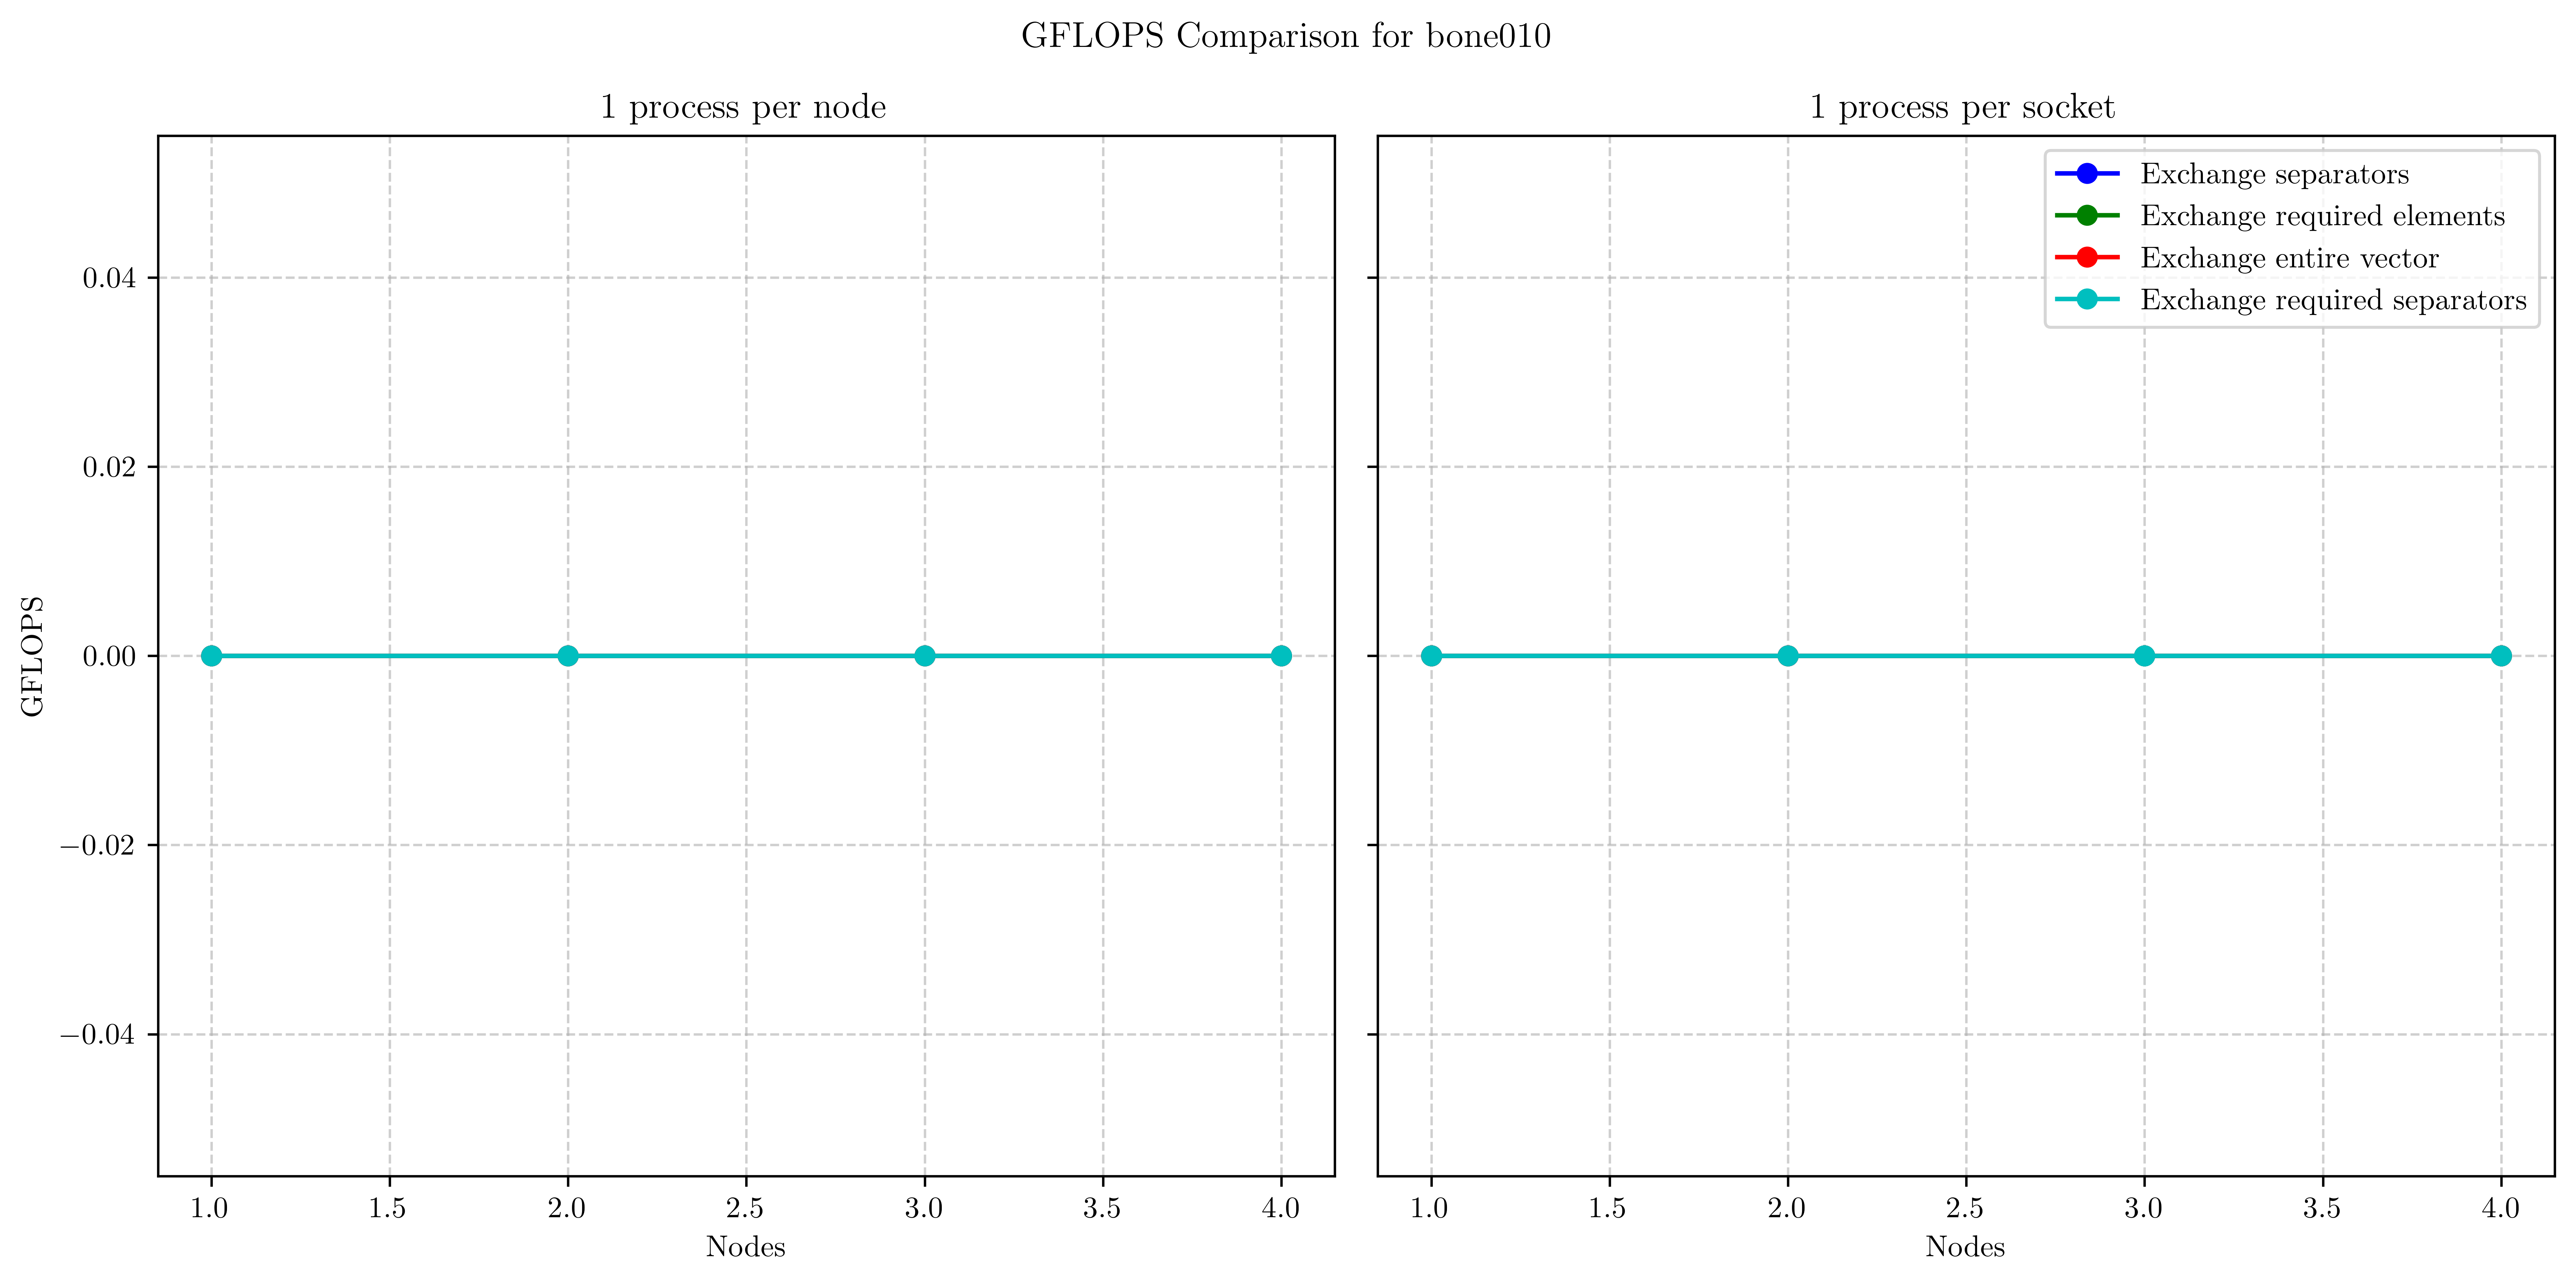
\includegraphics[width=0.23\textwidth]{bone010.png}%
    } &
    \subcaptionbox{\tiny{af\_shell10}\label{fig:af_shell10}}{%
      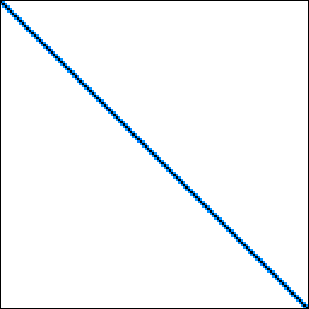
\includegraphics[width=0.23\textwidth]{af_shell10.png}%
    } &
    \subcaptionbox{\tiny{Serena}\label{fig:Serena}}{%
      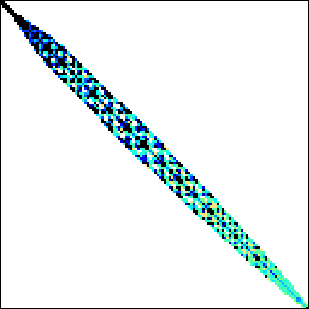
\includegraphics[width=0.23\textwidth]{Serena.png}%
    } &
    \subcaptionbox{\tiny{Long\_Coup\_dt0}\label{fig:Long_Coup_dt0}}{%
      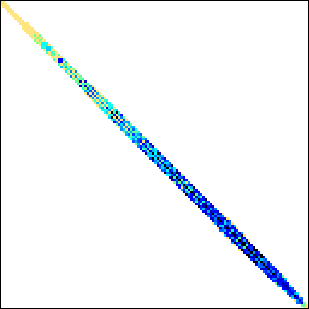
\includegraphics[width=0.23\textwidth]{Long_Coup_dt0.png}%
    } \\[6pt] % a little extra vertical gap
    \subcaptionbox{\tiny{dielFilterV3real}\label{fig:dielFilterV3real}}{%
      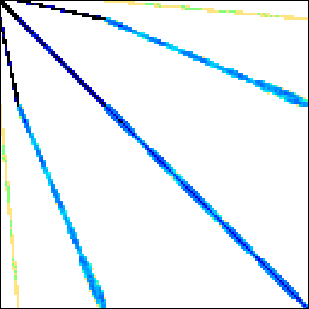
\includegraphics[width=0.23\textwidth]{dielFilterV3real.png}%
    } &
    \subcaptionbox{\tiny{Cube\_Coup\_dt0}\label{fig:Cube_Coup_dt0_1}}{%
      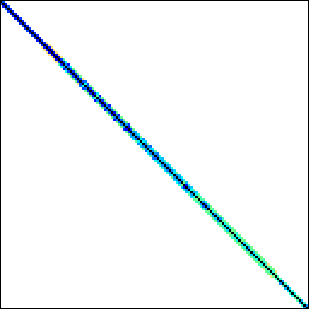
\includegraphics[width=0.23\textwidth]{Cube_Coup_dt0.png}%
    } &
    \subcaptionbox{\tiny{Bump\_2911}\label{fig:Bump_2911}}{%
      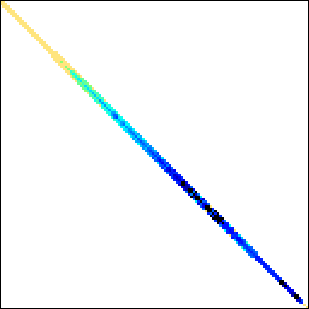
\includegraphics[width=0.23\textwidth]{Bump_2911.png}%
    } &
    \subcaptionbox{\tiny{nlpkkt200}\label{fig:nlpkkt200}}{%
      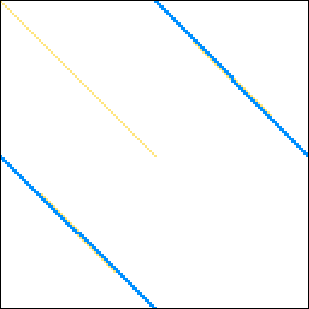
\includegraphics[width=0.23\textwidth]{nlpkkt200.png}%
    }
  \end{tabular}
  \caption{Overview of all eight images.}
  \label{fig:all_images}
\end{figure}

\begin{figure}[H]
    \centering
    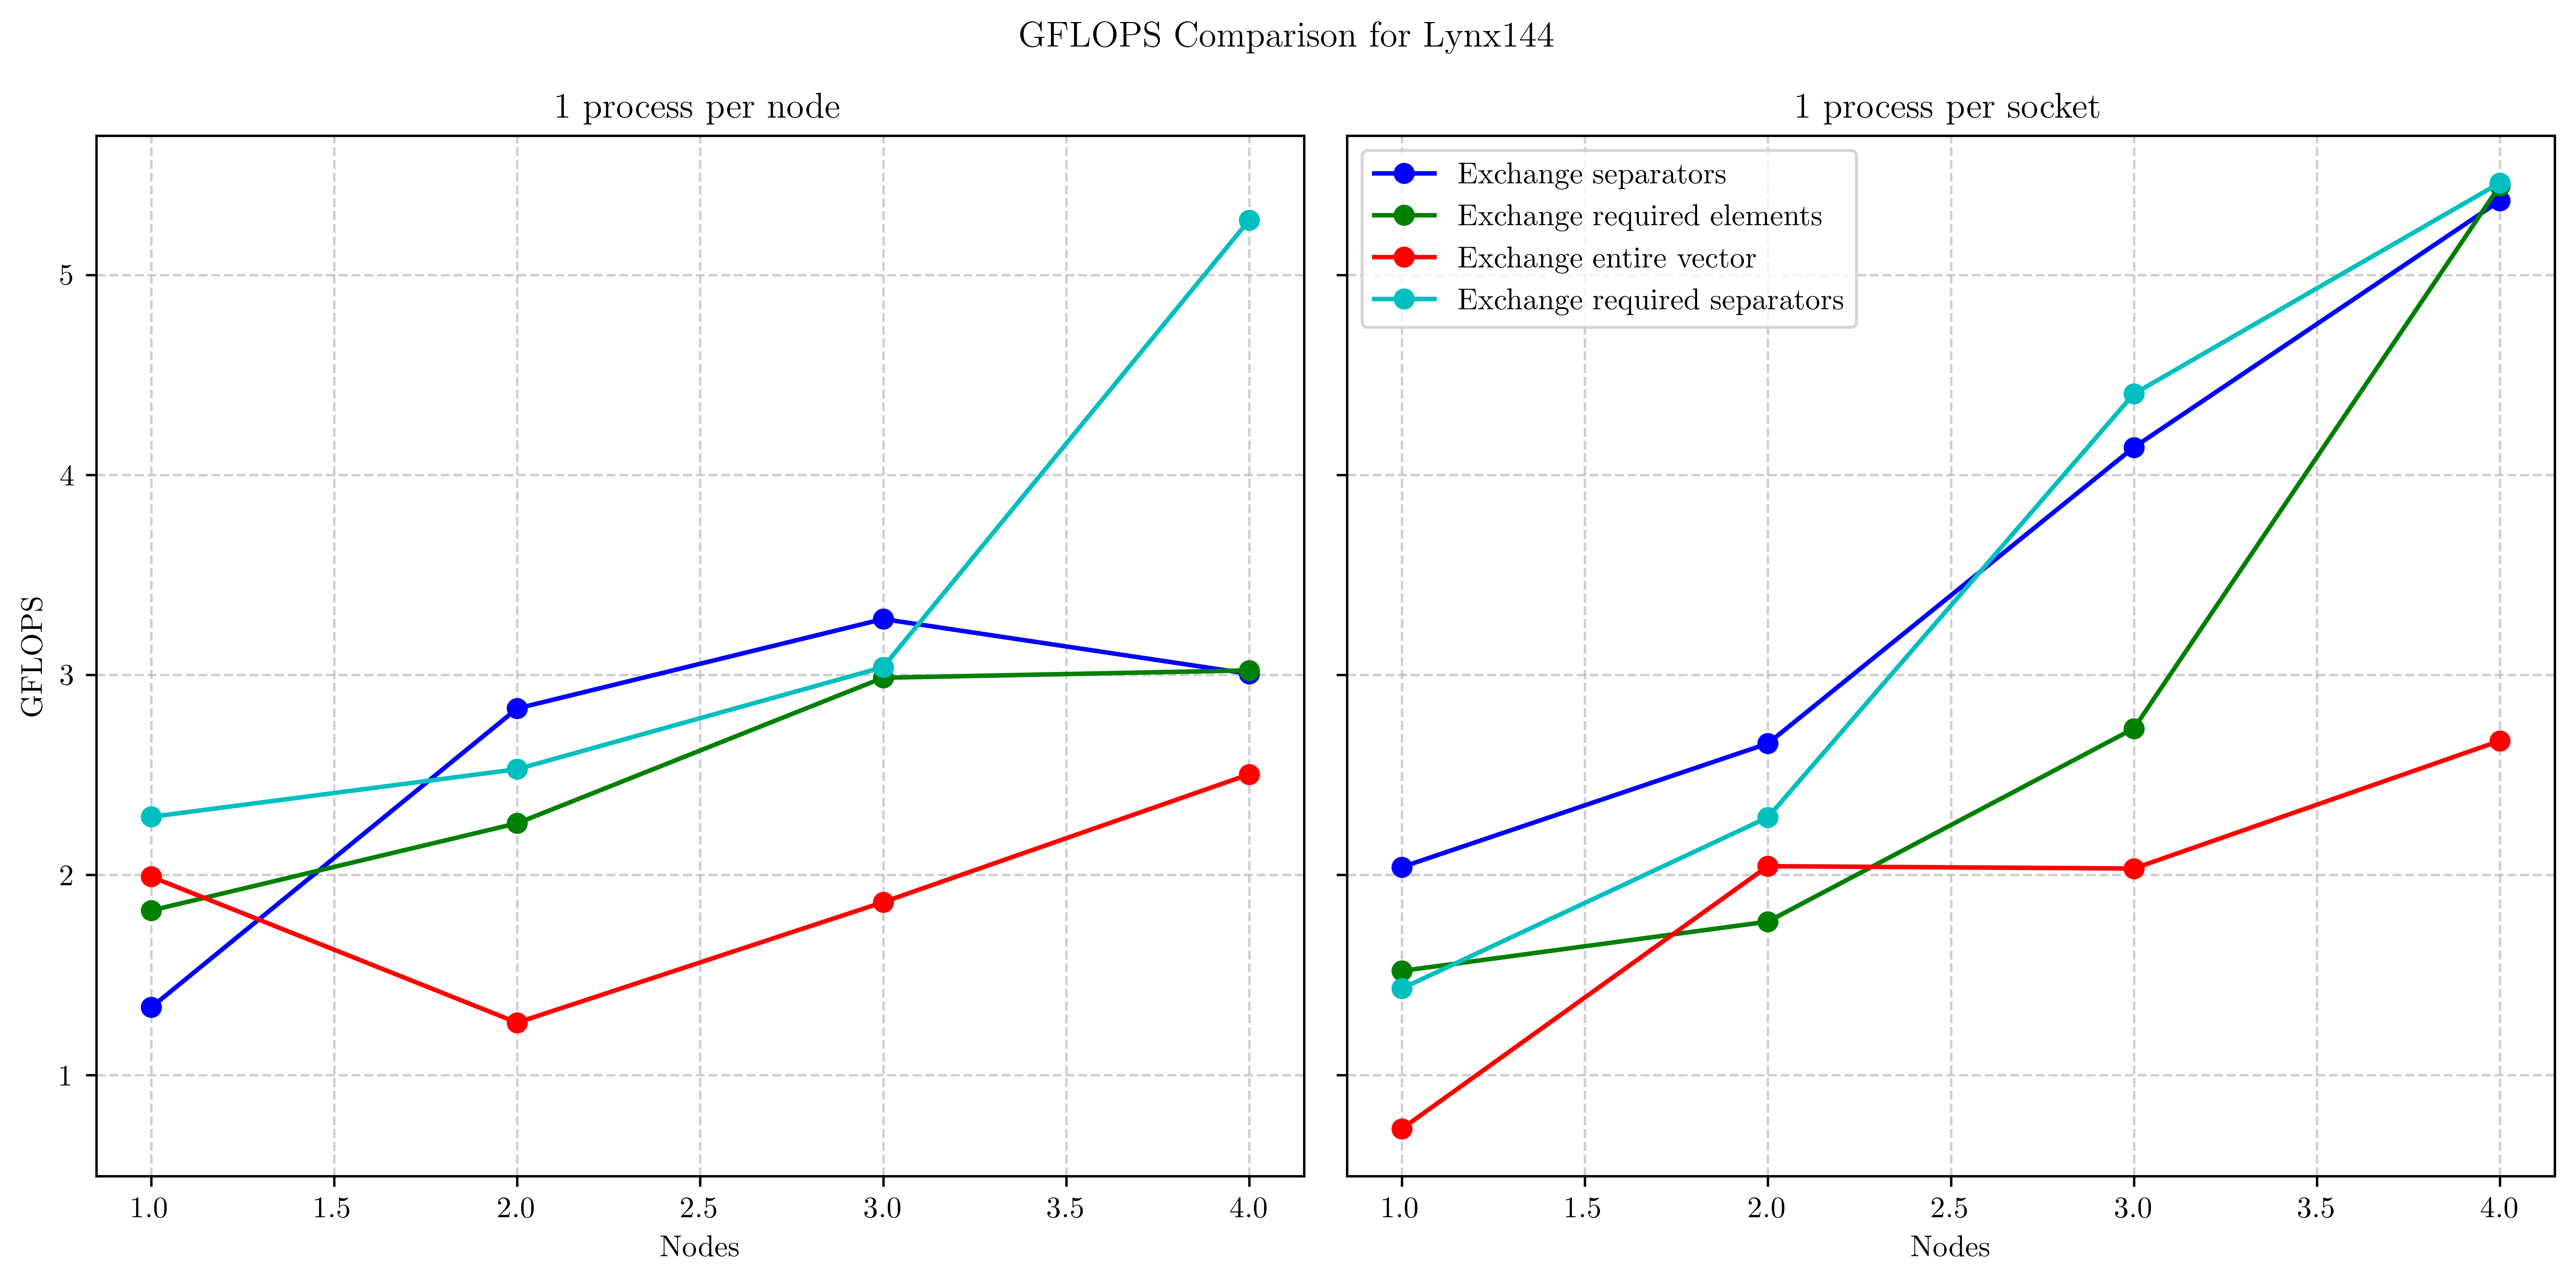
\includegraphics[width=0.95\textwidth]{Lynx144.png}
    \caption{SpMV performance with 1 process vs 2 processes per node on Lynx144}
    \label{fig:lynx144gflops}
\end{figure}

\begin{figure}[H]
    \centering
    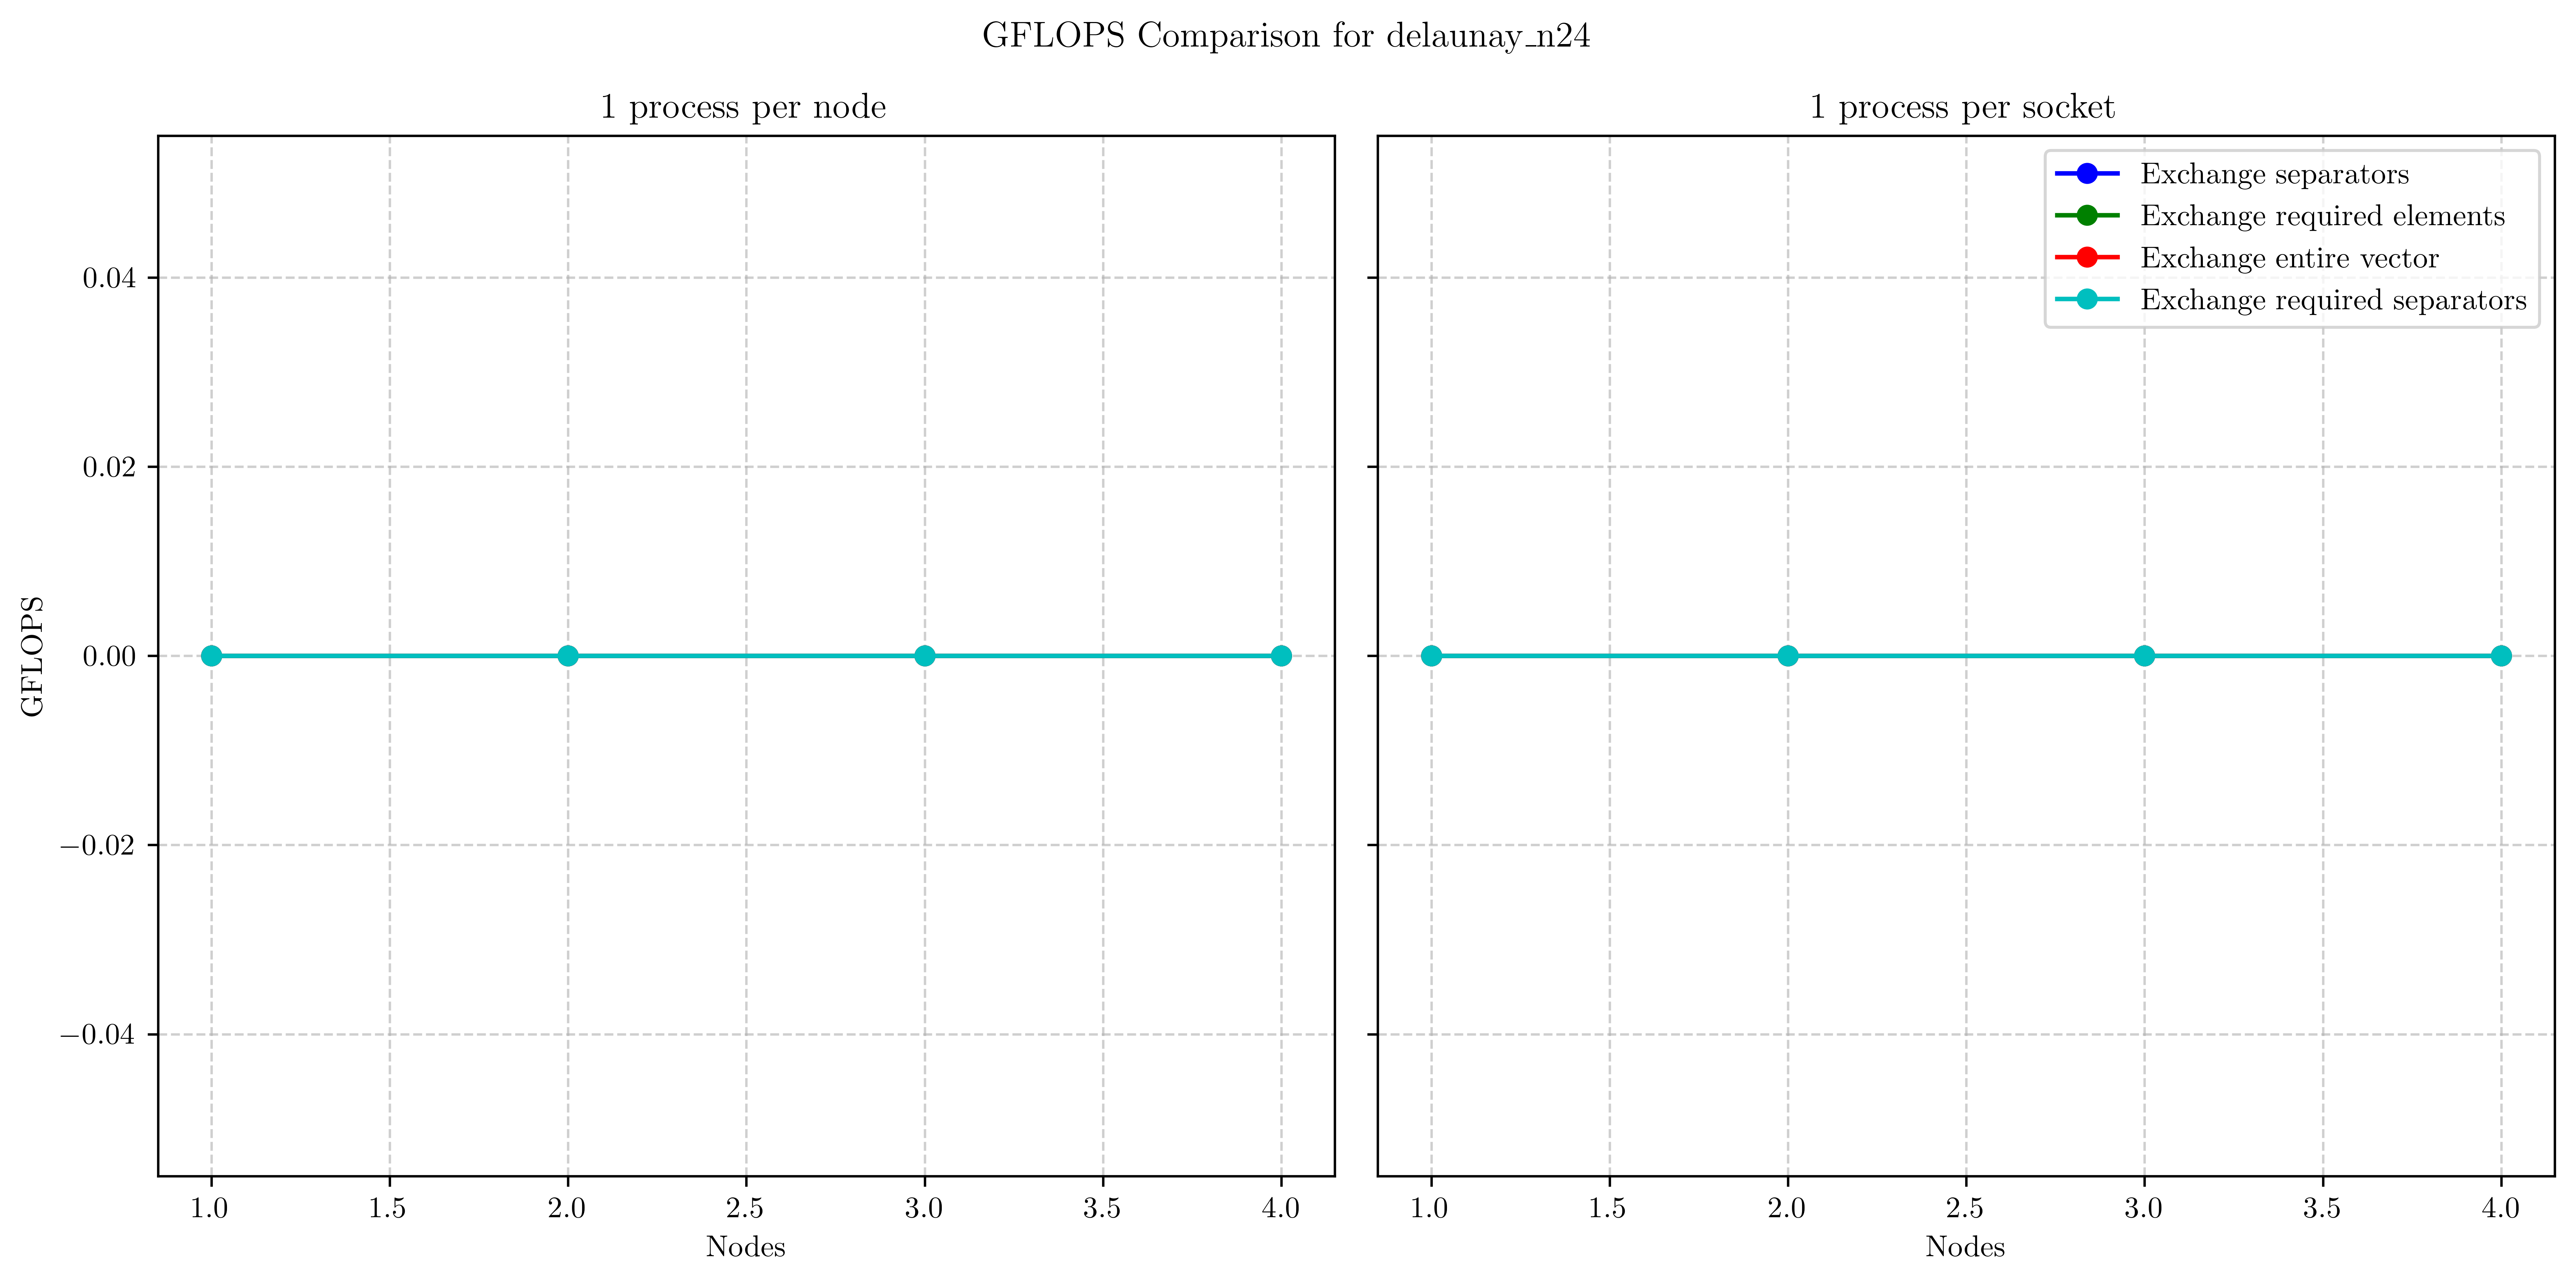
\includegraphics[width=0.95\textwidth]{delaunay_n24.png}
    \caption{SpMV performance with 1 process vs 2 processes per node on delaynay\_n24}
    \label{fig:delaunayflops}
\end{figure}

\begin{figure}[H]
    \begin{center}
        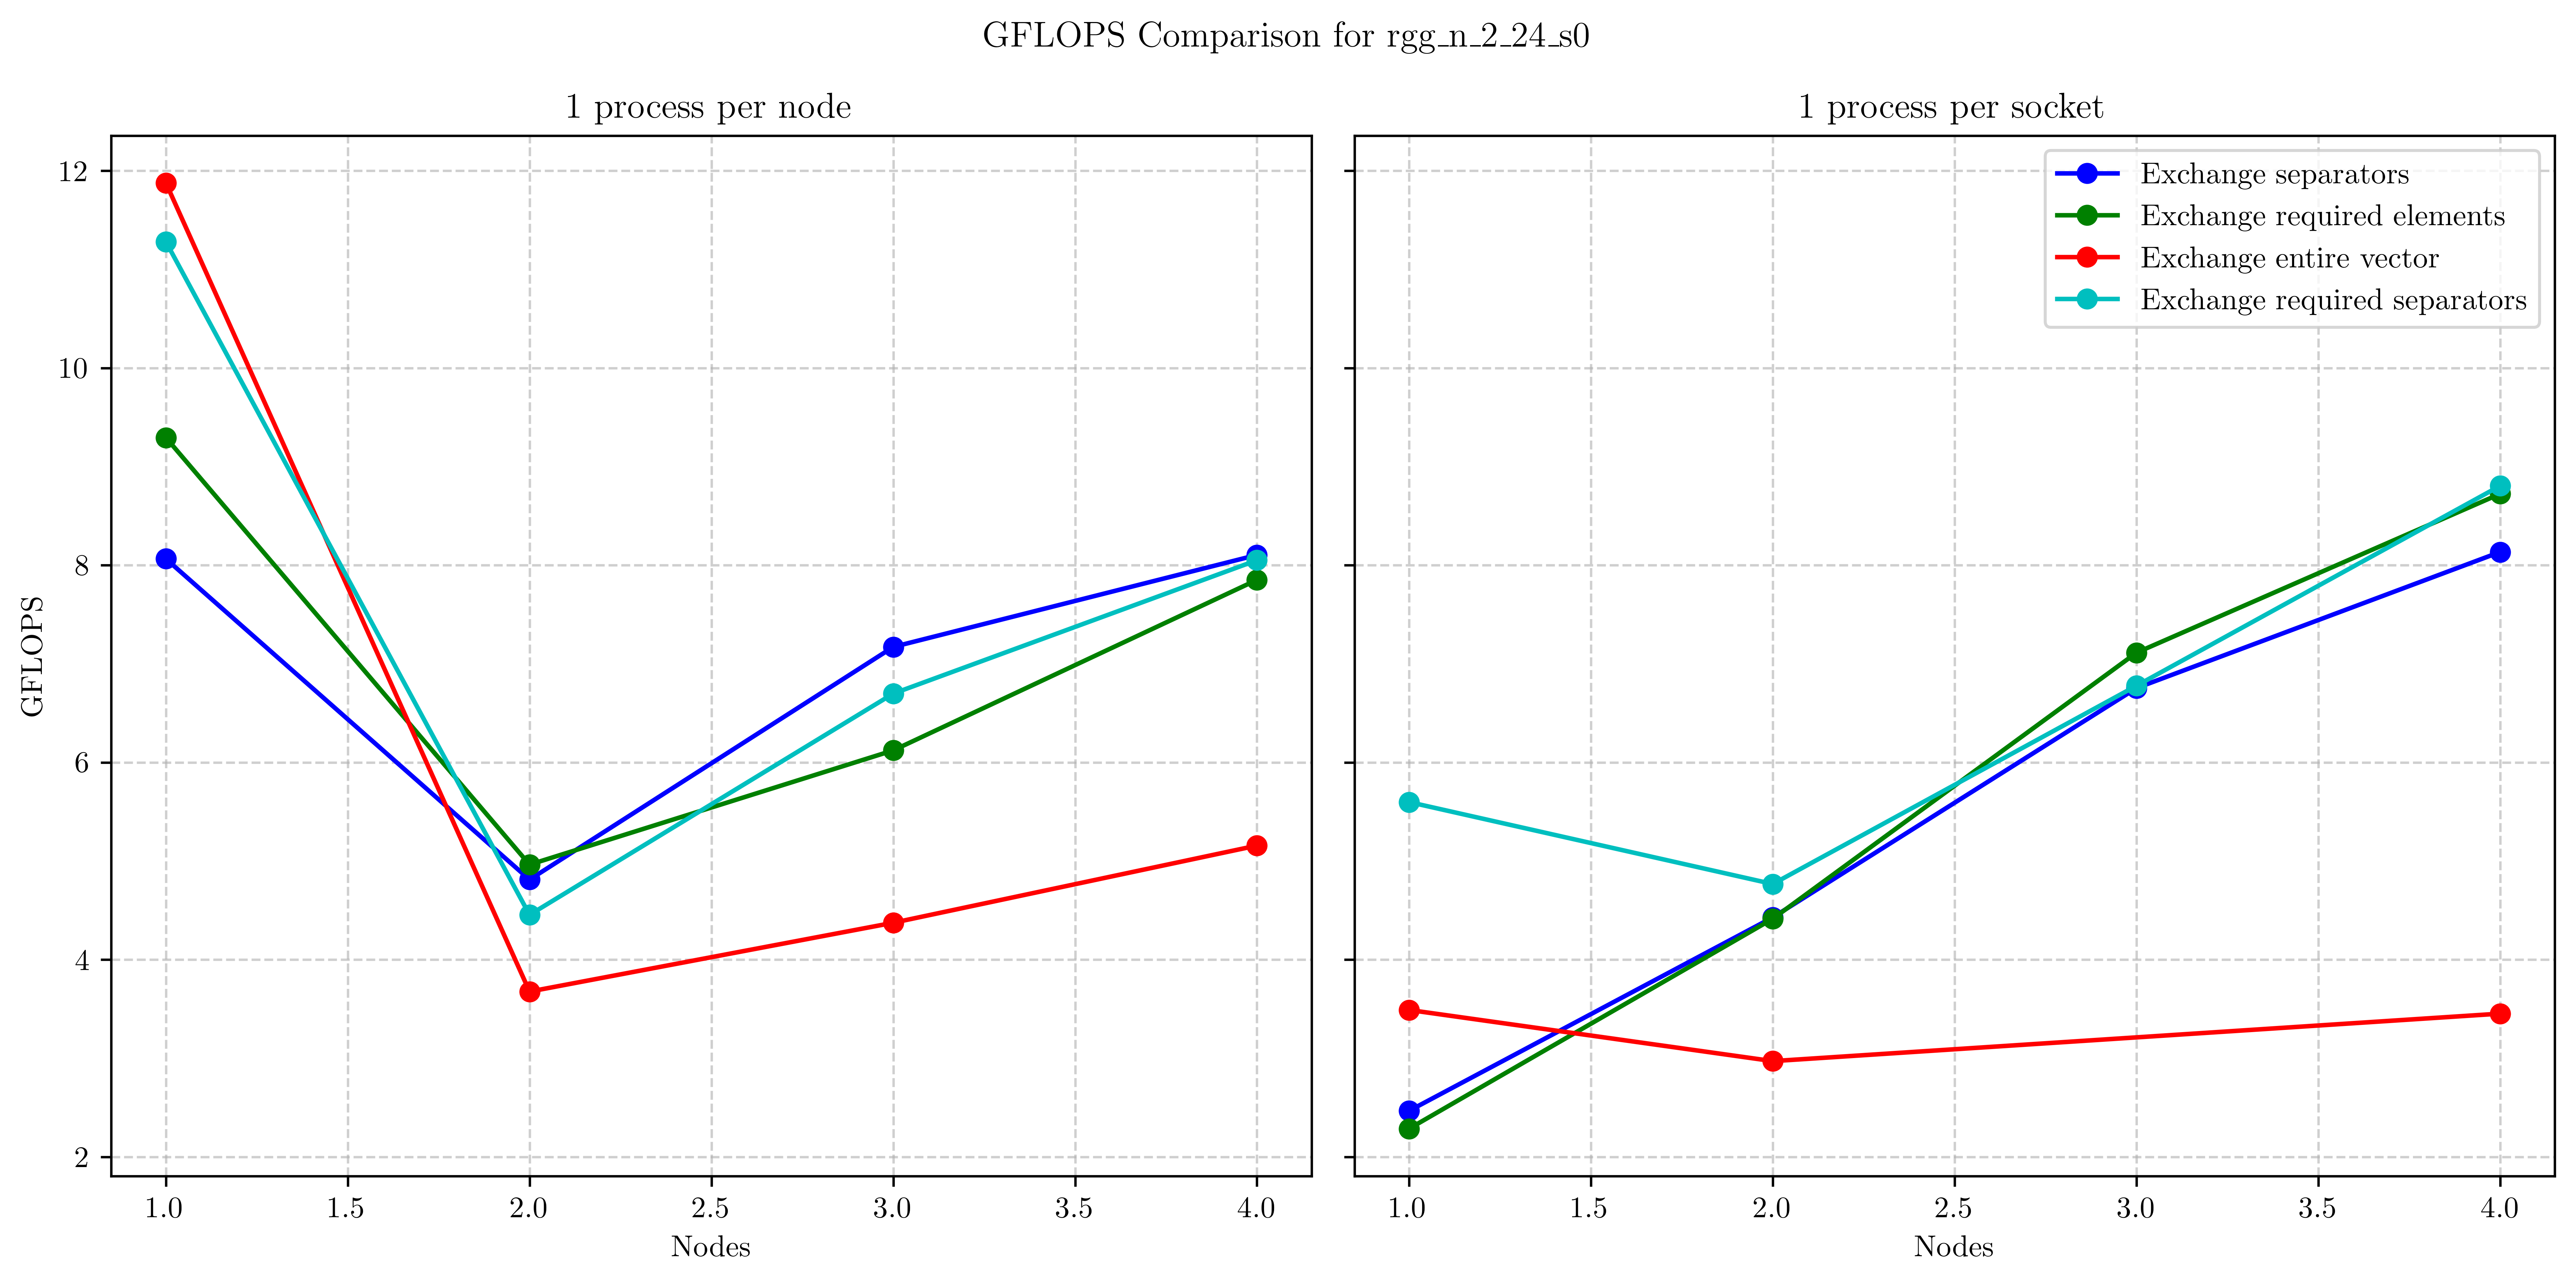
\includegraphics[width=0.95\textwidth]{rgg_n_2_24_s0}
    \end{center}
    \caption{SpMV performance with 1 process vs 2 processes per node on rgg\_n\_2\_24\_s0}
    \label{fig:rgg_n_2_24_s0}
\end{figure}

\begin{figure}[H]
    \begin{center}
        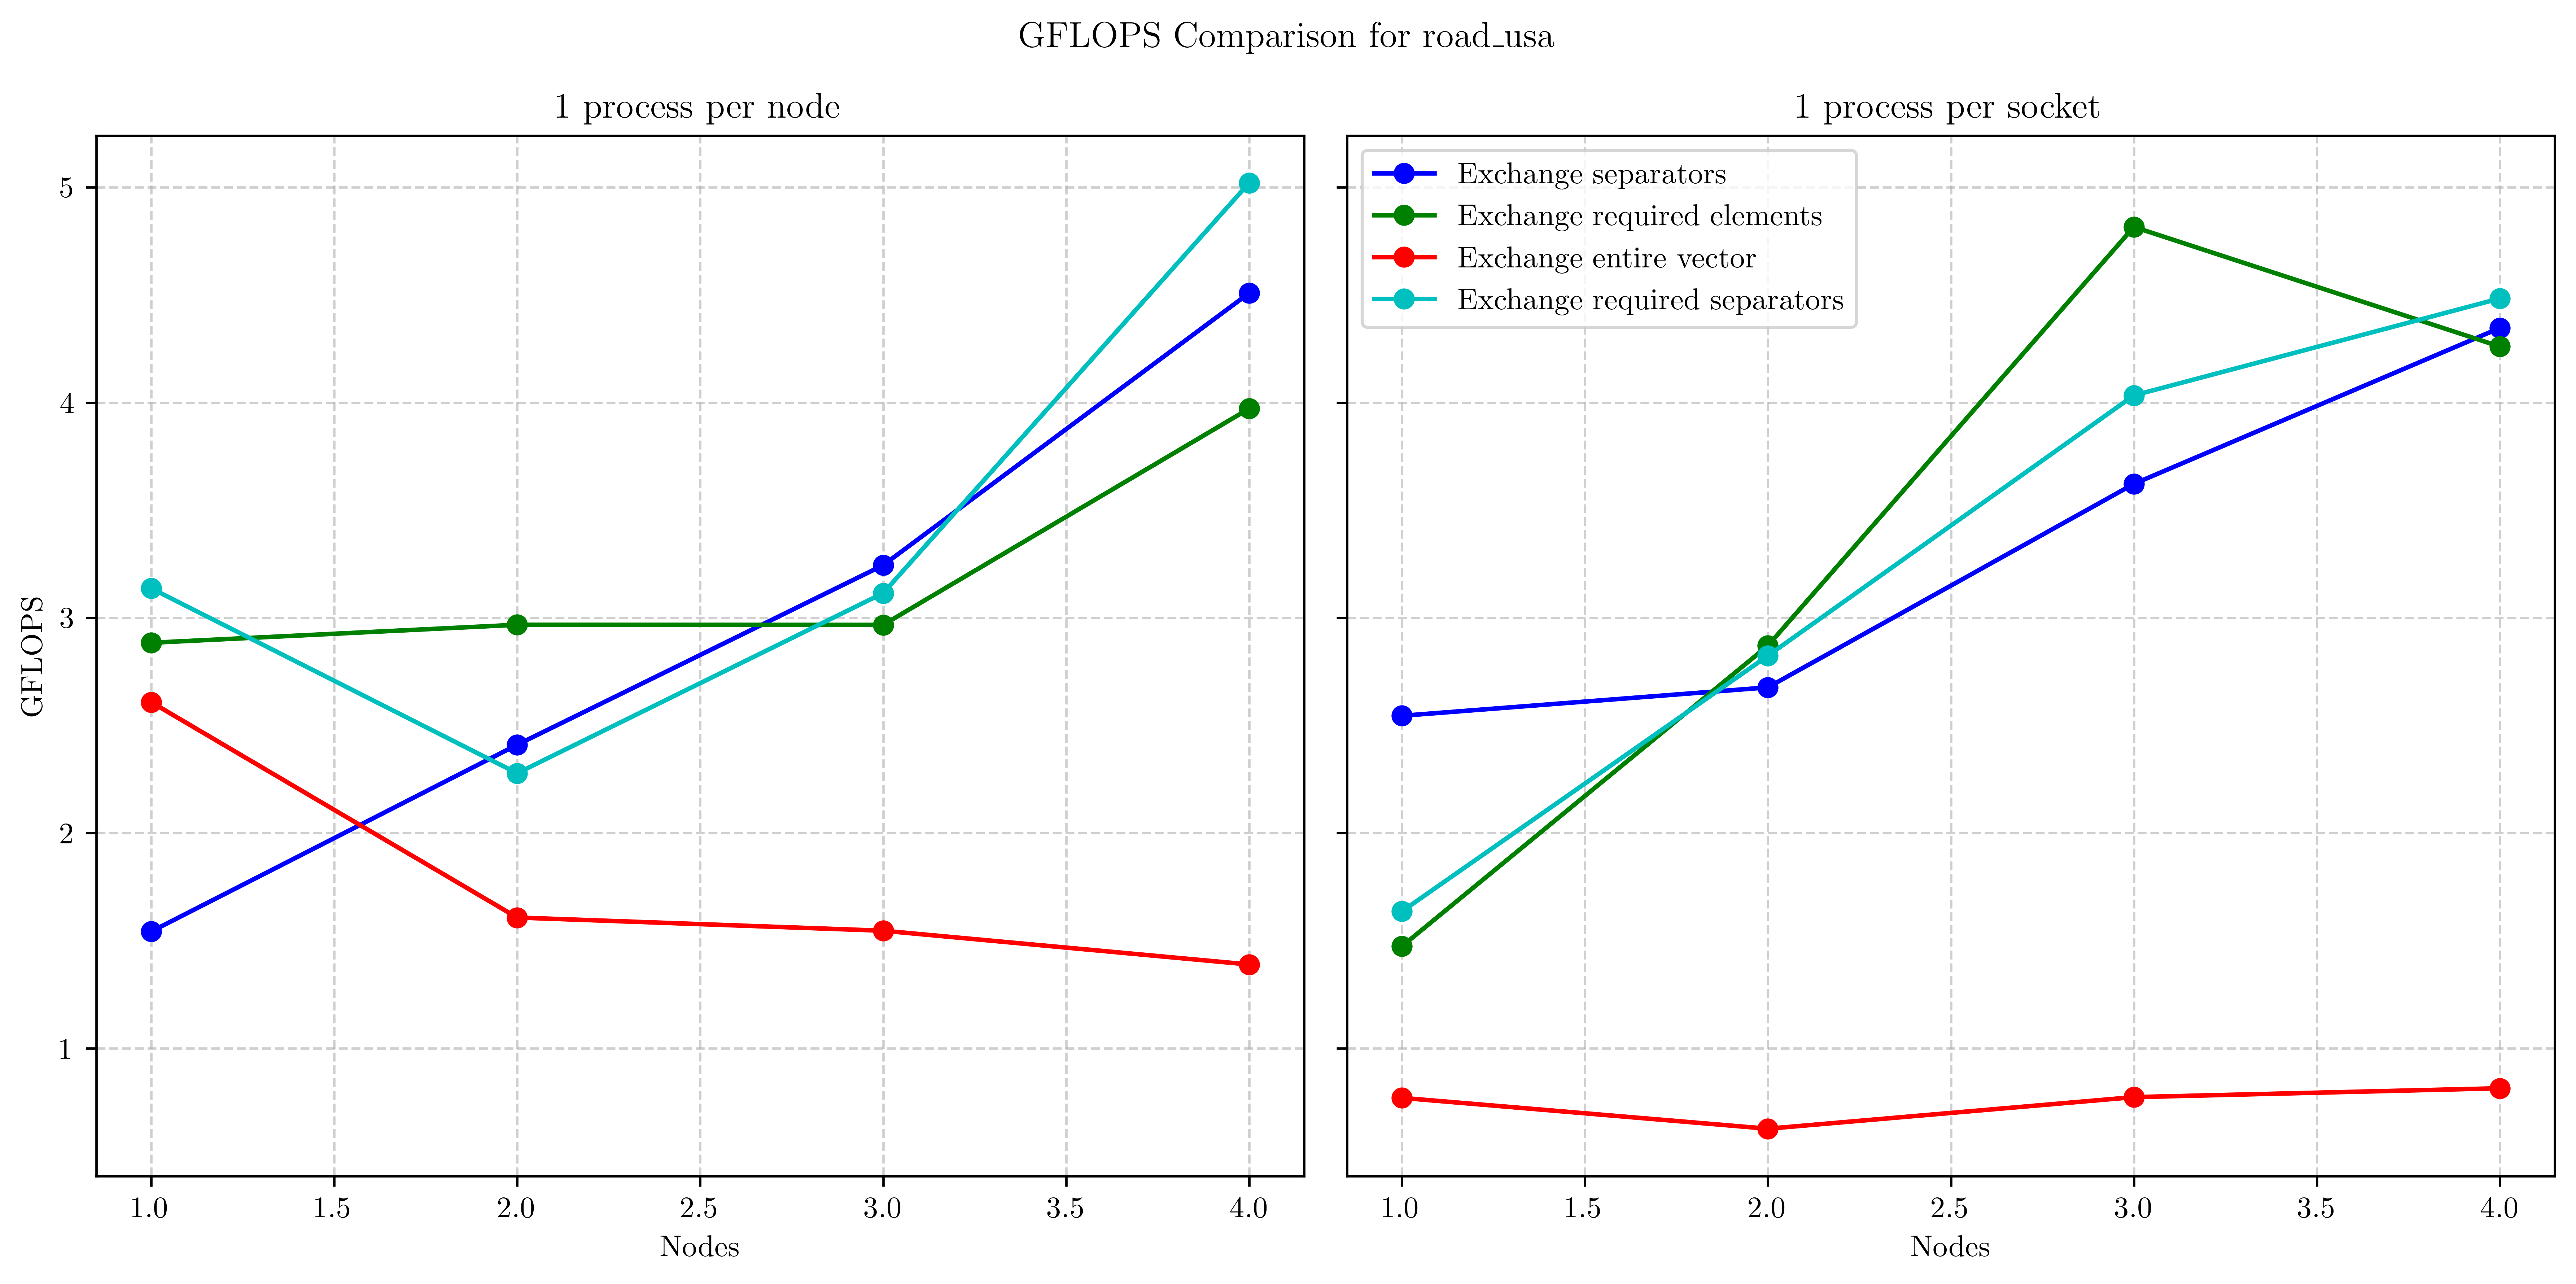
\includegraphics[width=0.95\textwidth]{road_usa}
    \end{center}
    \caption{SpMV performance with 1 process vs 2 processes per node on road\_usa}
    \label{fig:road_usa}
\end{figure}


\section{GFLOPS \romeq}

\begin{figure}[H]
    \begin{center}
        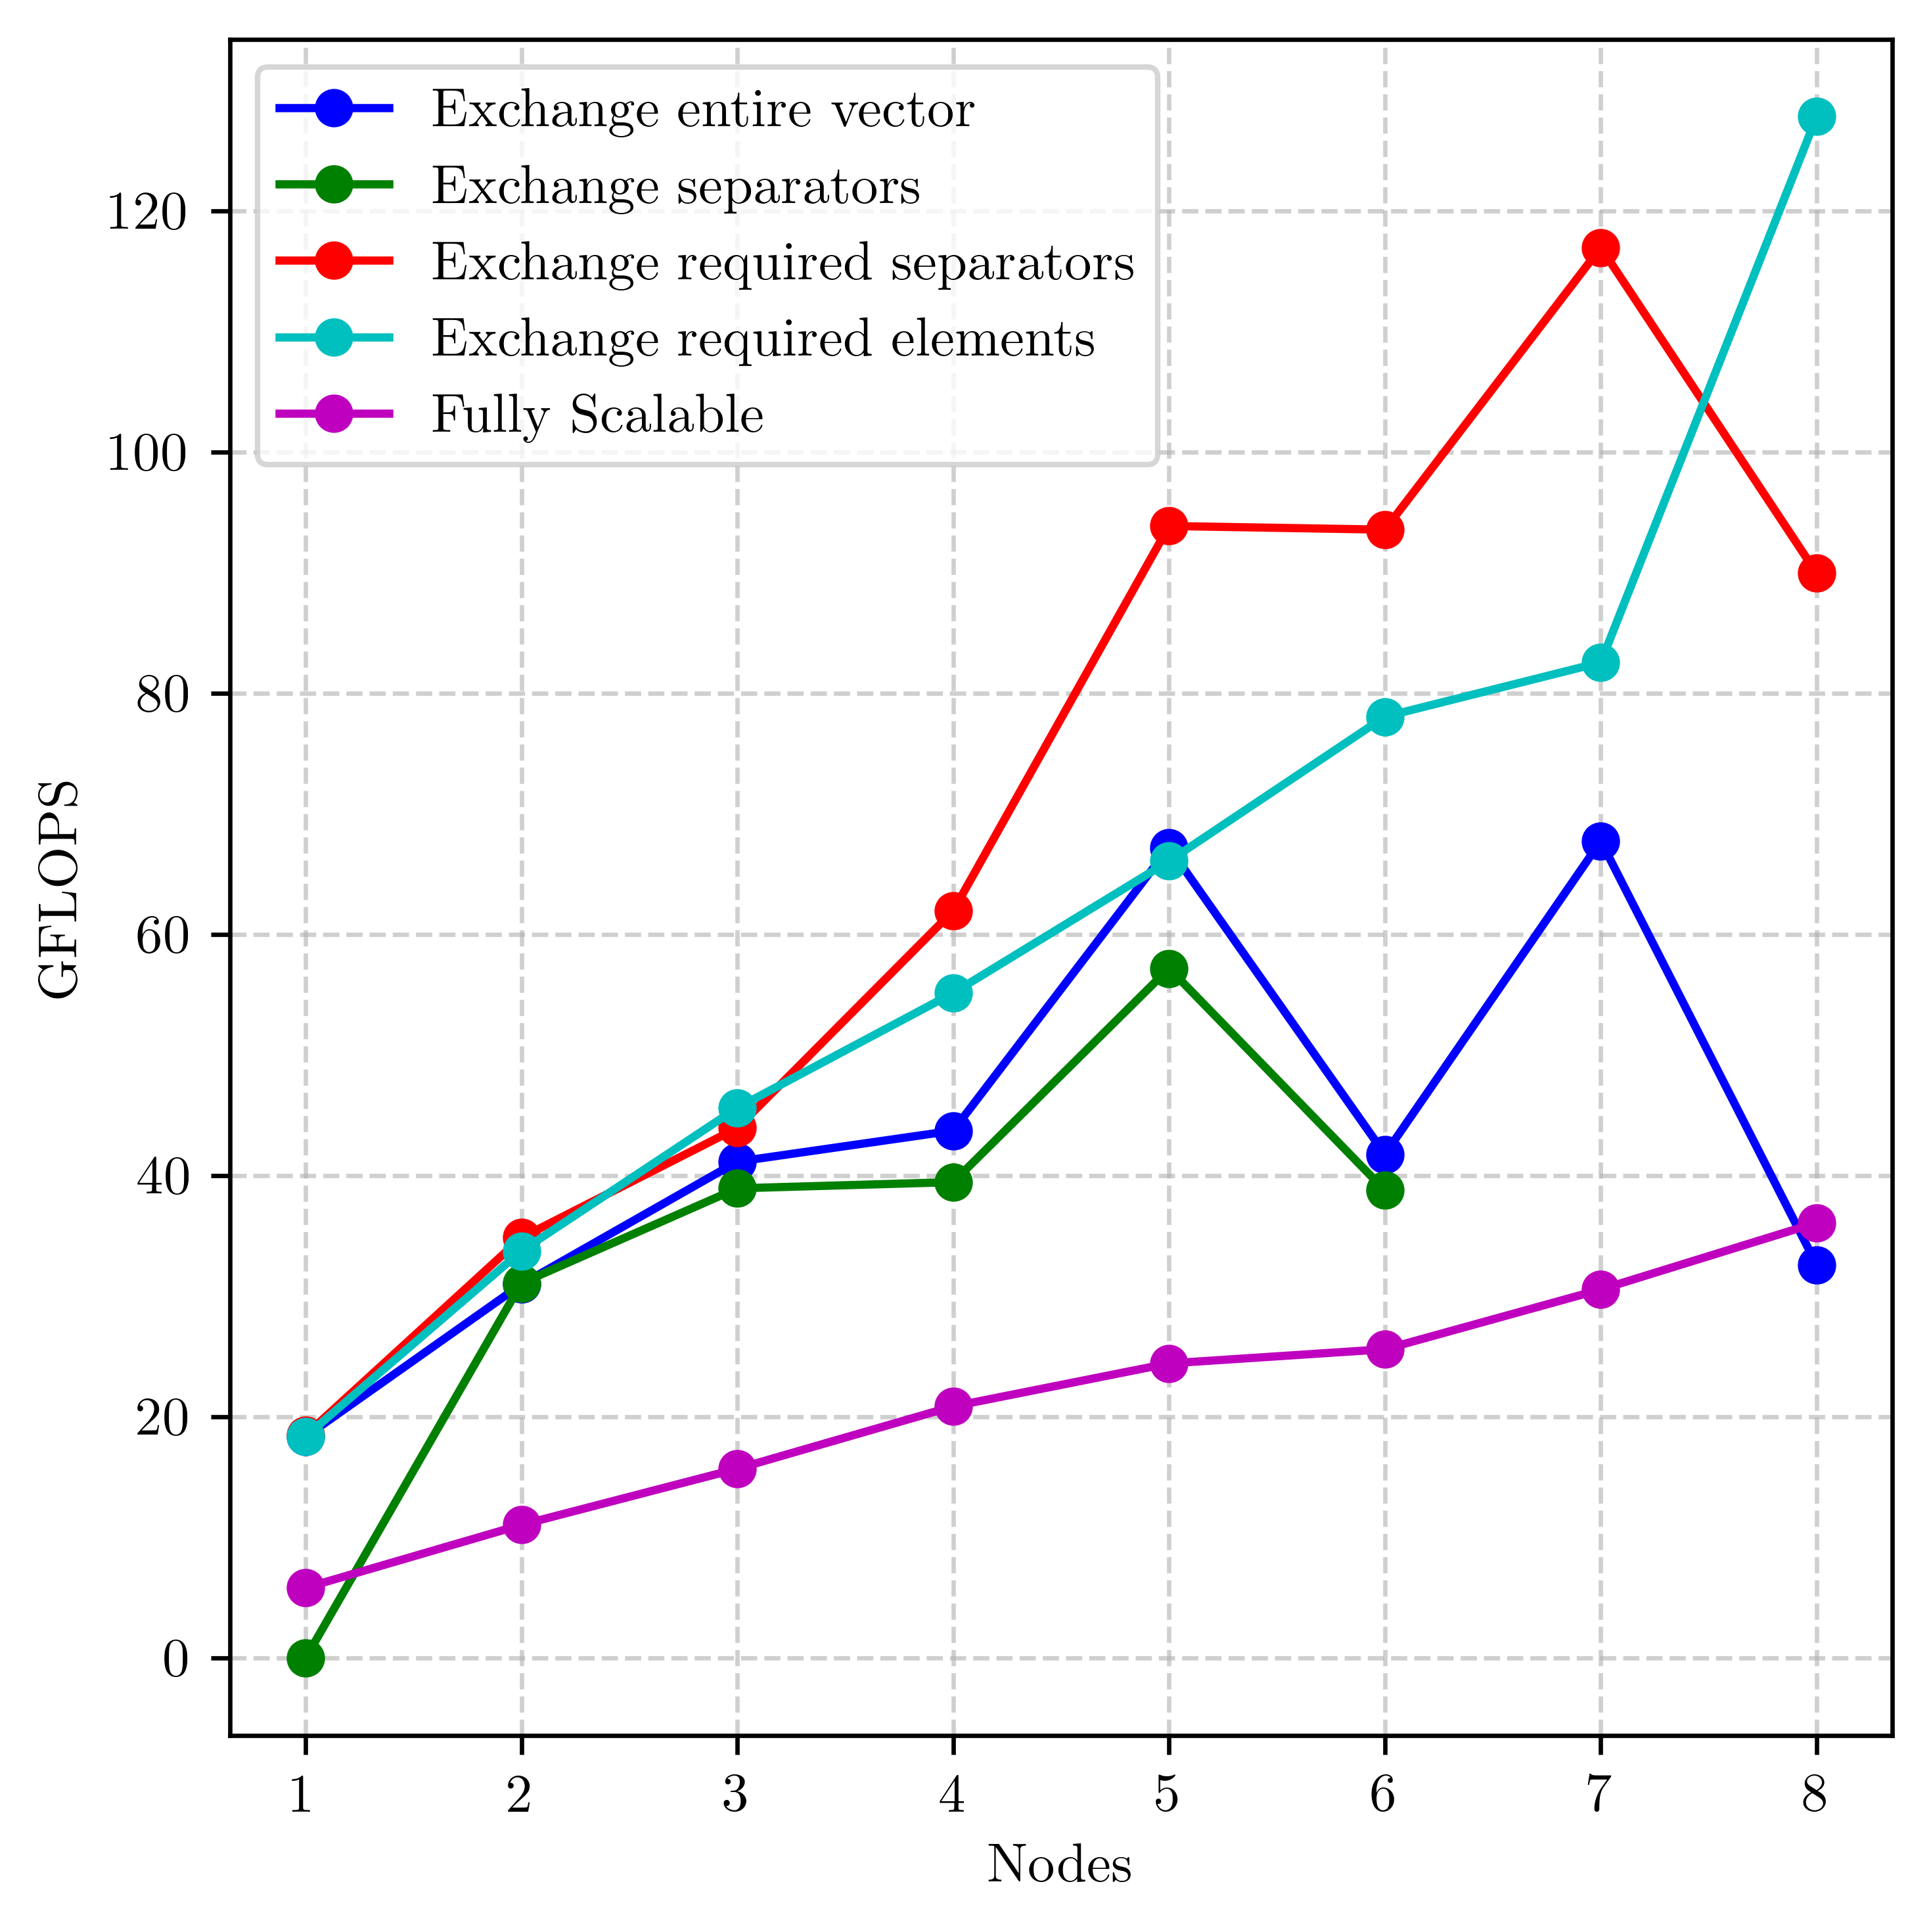
\includegraphics[width=0.95\textwidth]{Serena_rome16q}
    \end{center}
    \caption{Serena}
    \label{fig:Serena_rome16q}
\end{figure}

\begin{figure}[H]
    \begin{center}
        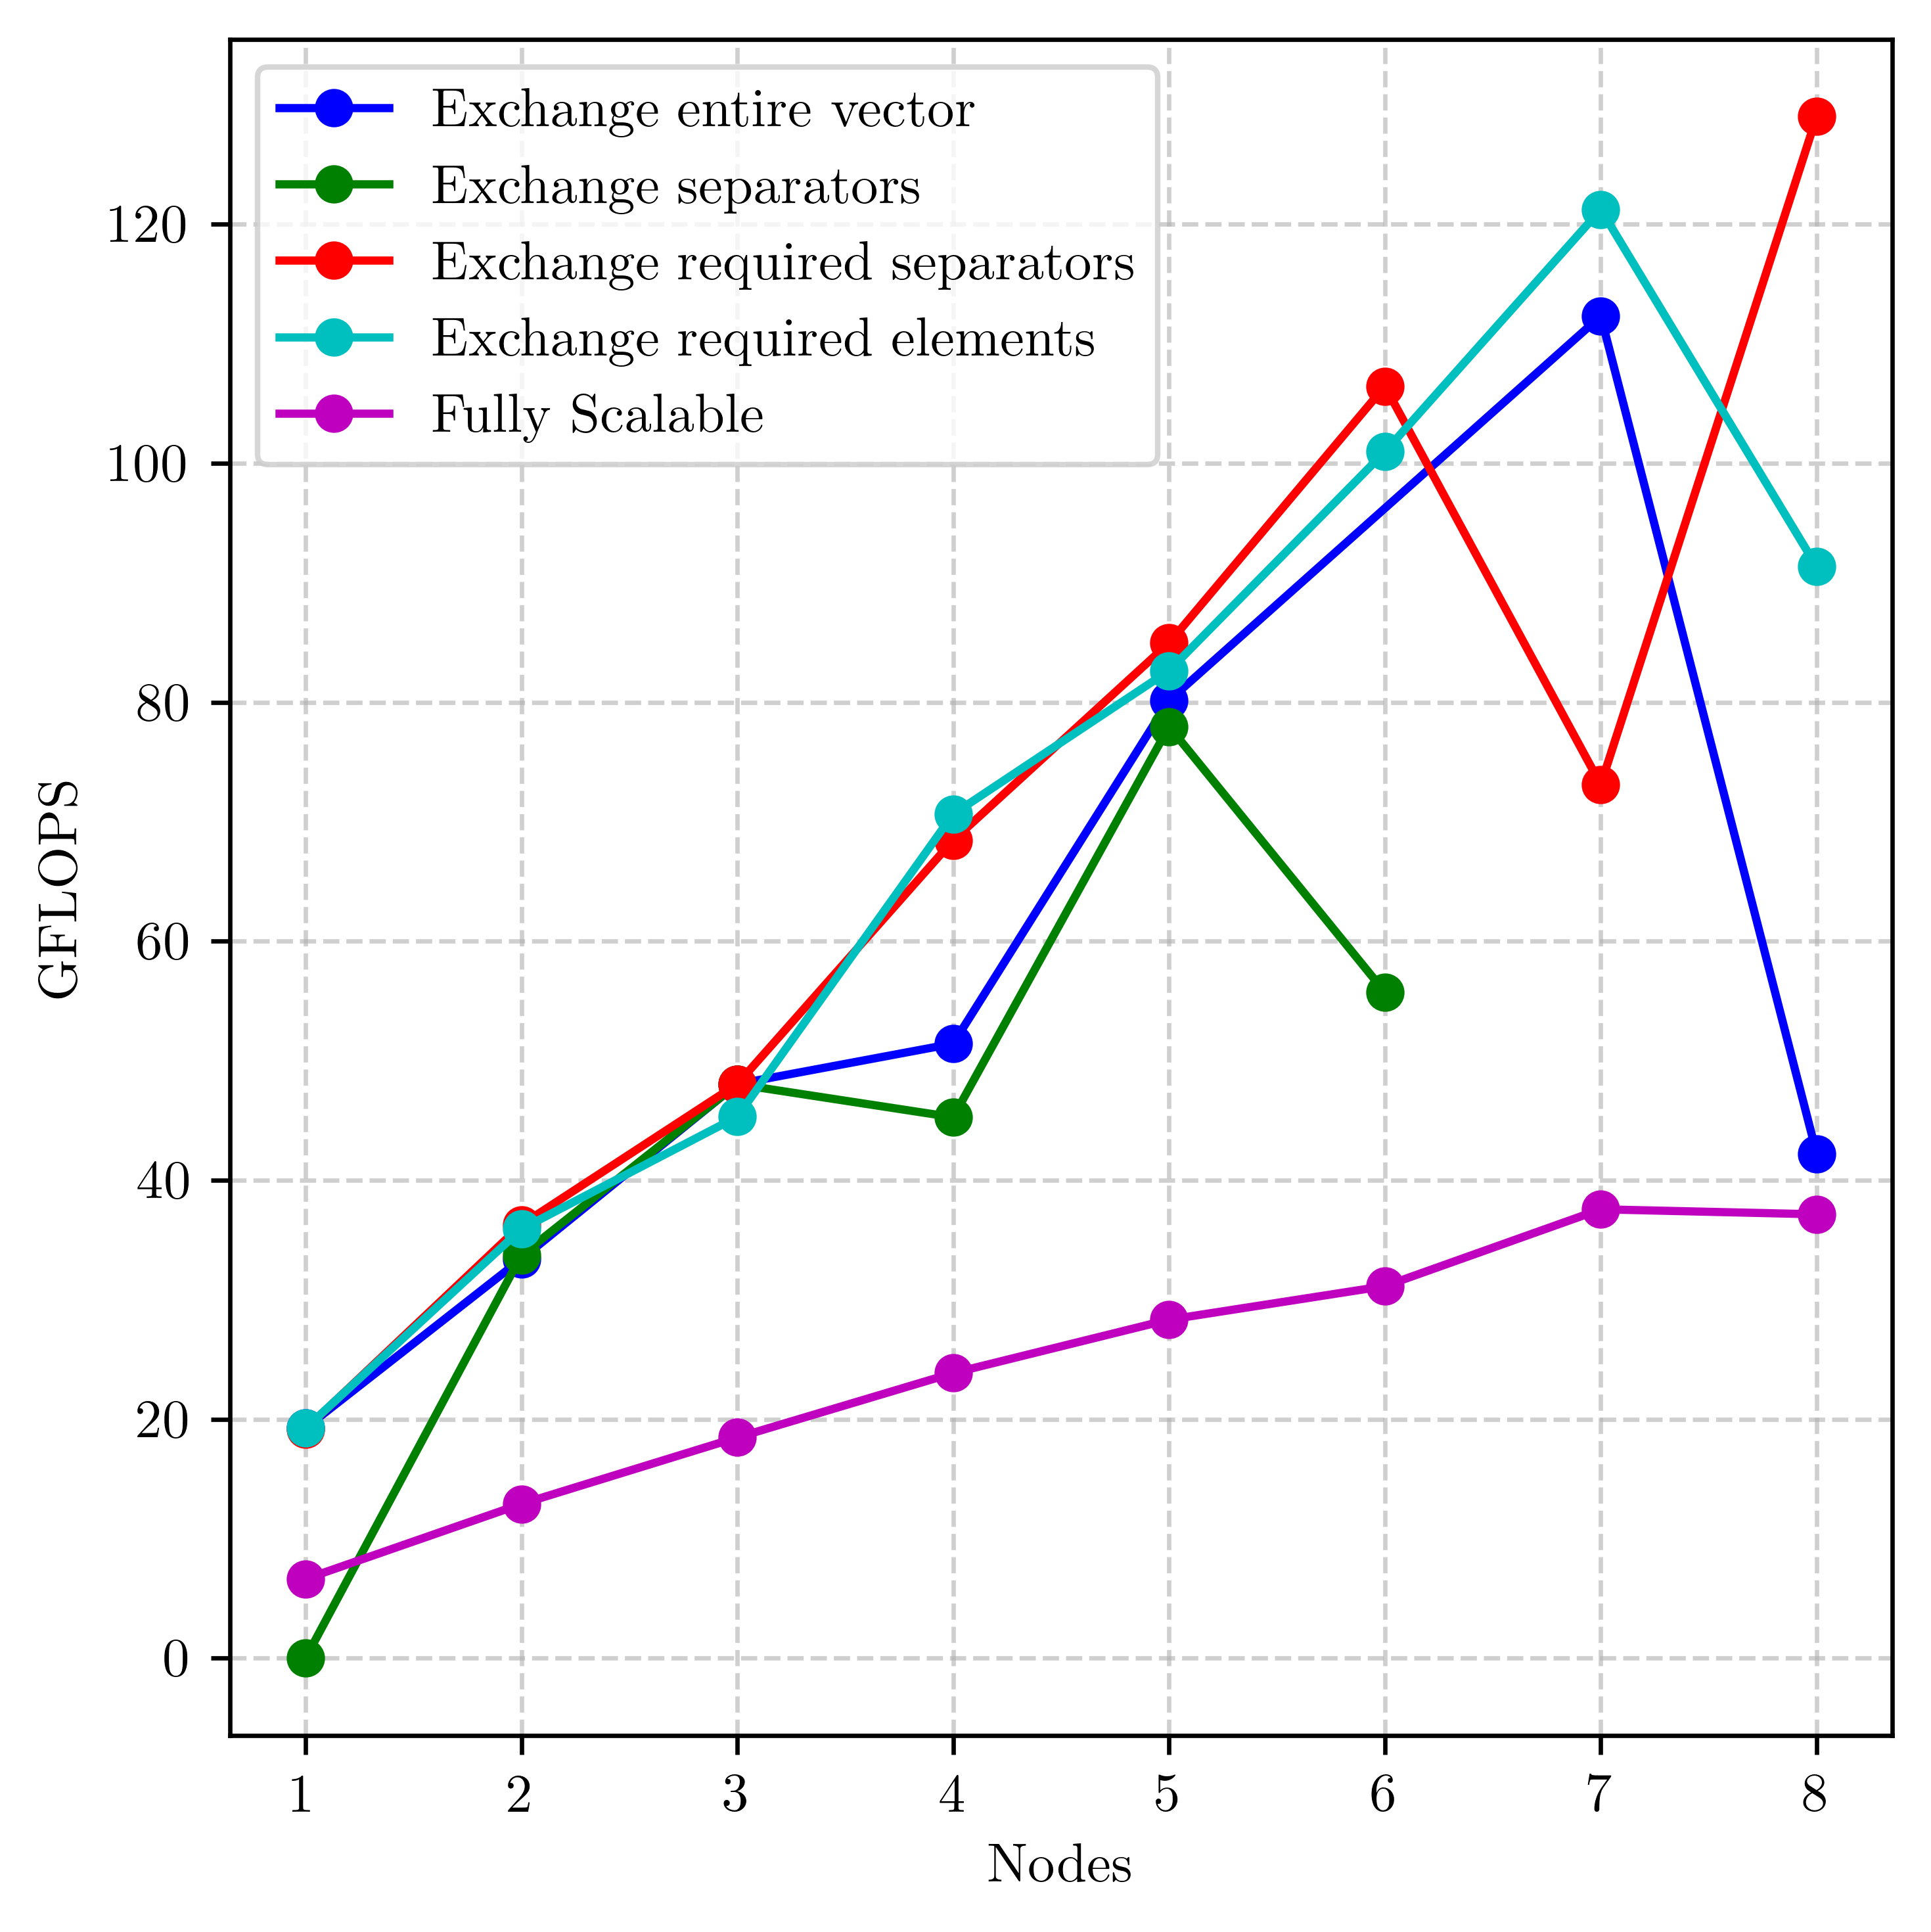
\includegraphics[width=0.95\textwidth]{bone010_rome16q}
    \end{center}
    \caption{bone010}
    \label{fig:bone010_rome16q}
\end{figure}

\begin{figure}[H]
    \begin{center}
        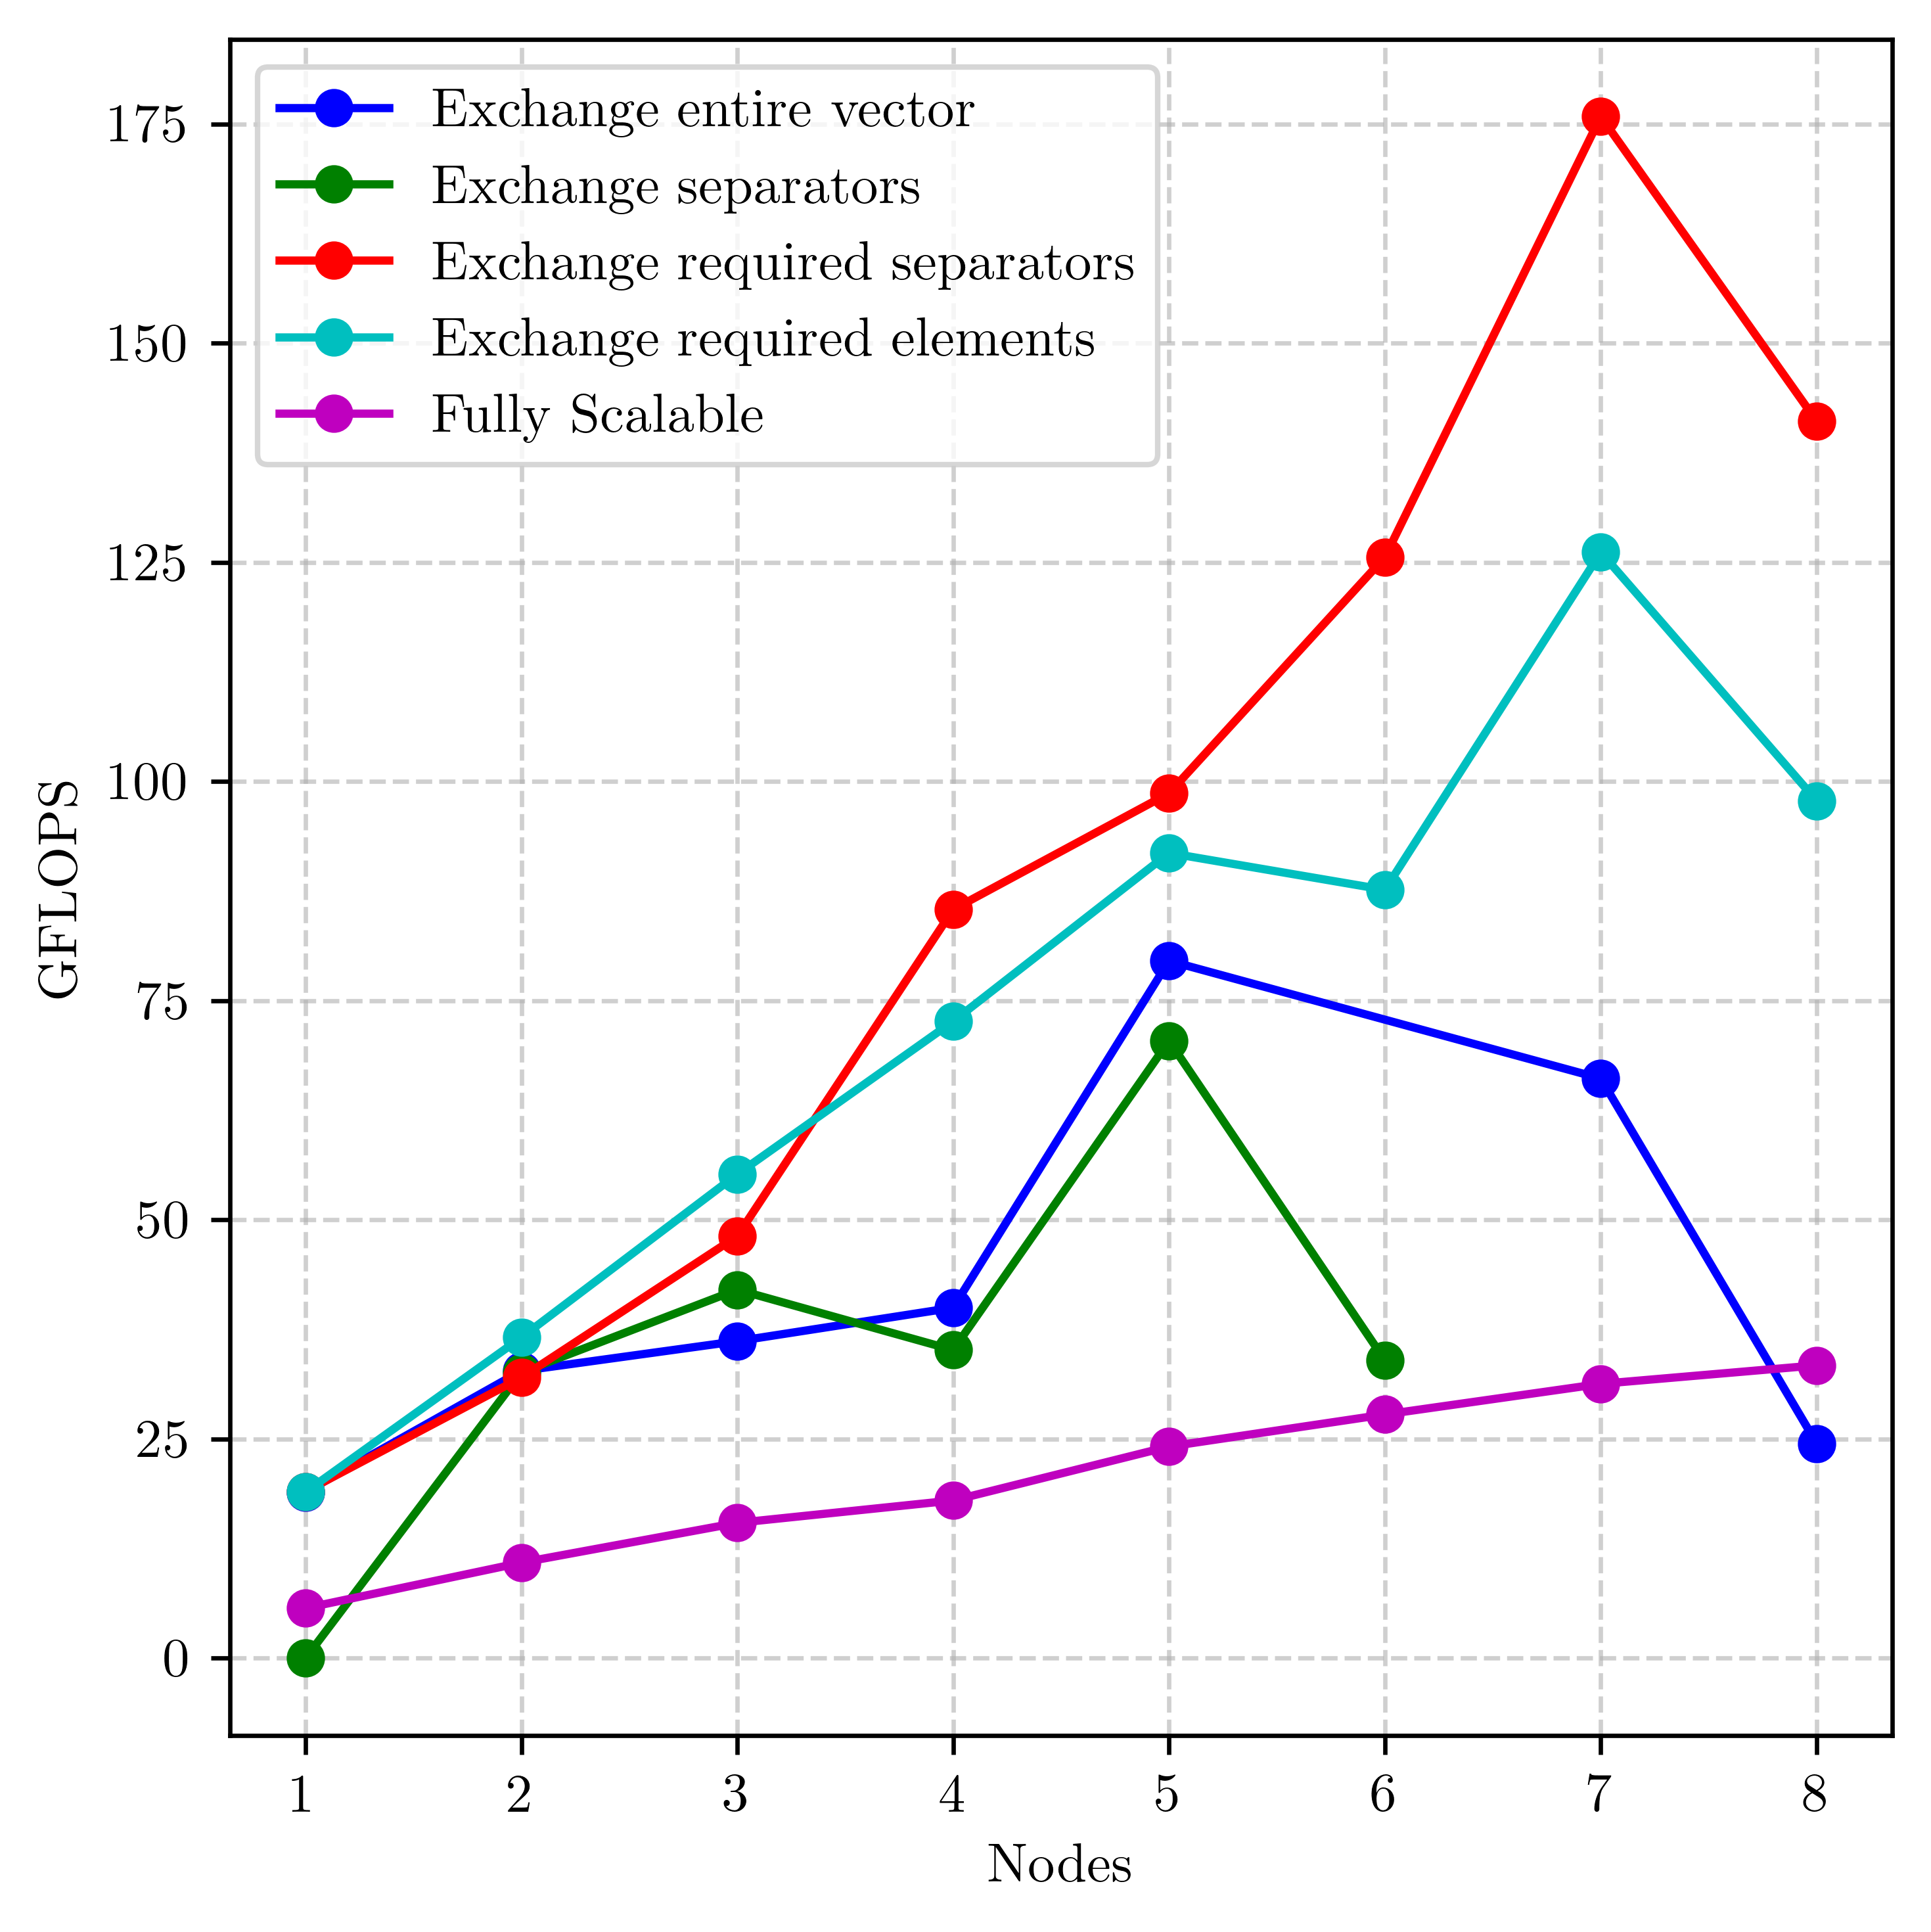
\includegraphics[width=0.95\textwidth]{af_shell10_rome16q}
    \end{center}
    \caption{af\_shell10}
    \label{fig:af_shell10_rome16q}
\end{figure}

\begin{figure}[H]
    \begin{center}
        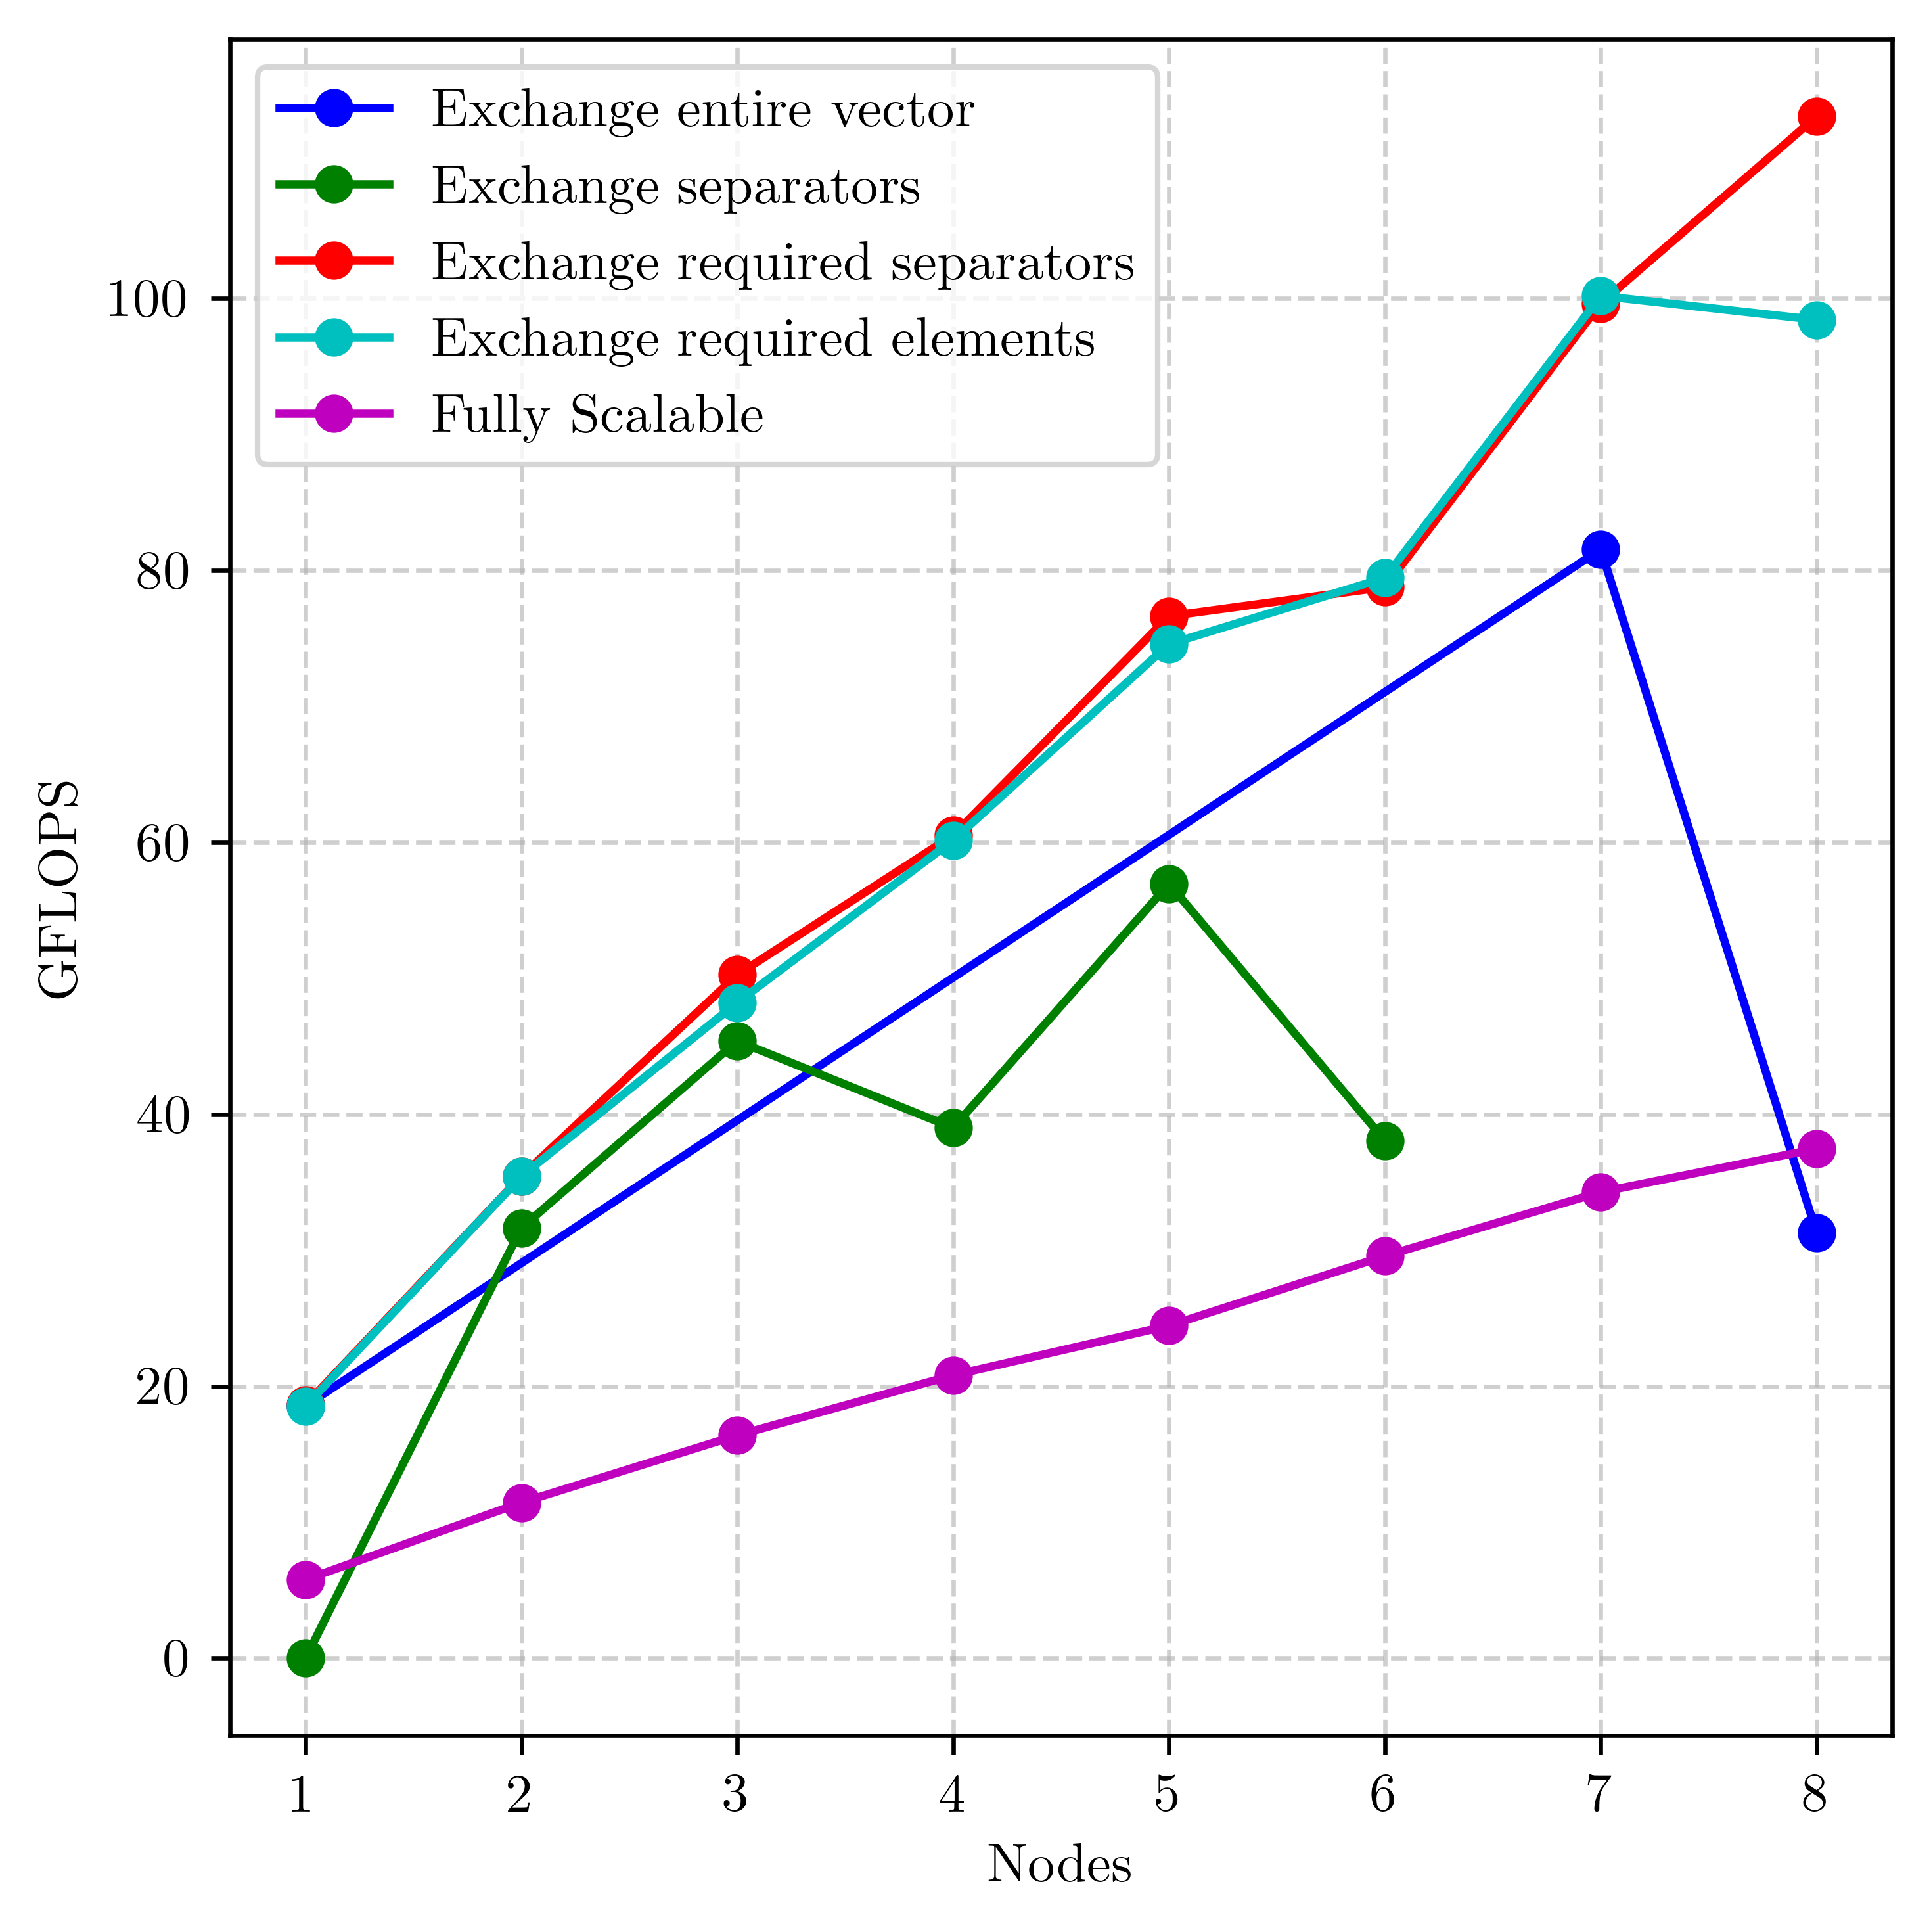
\includegraphics[width=0.95\textwidth]{Bump_2911_rome16q}
    \end{center}
    \caption{Bump\_2911}
    \label{fig:Bump_2911_rome16q}
\end{figure}

\begin{figure}[H]
    \begin{center}
        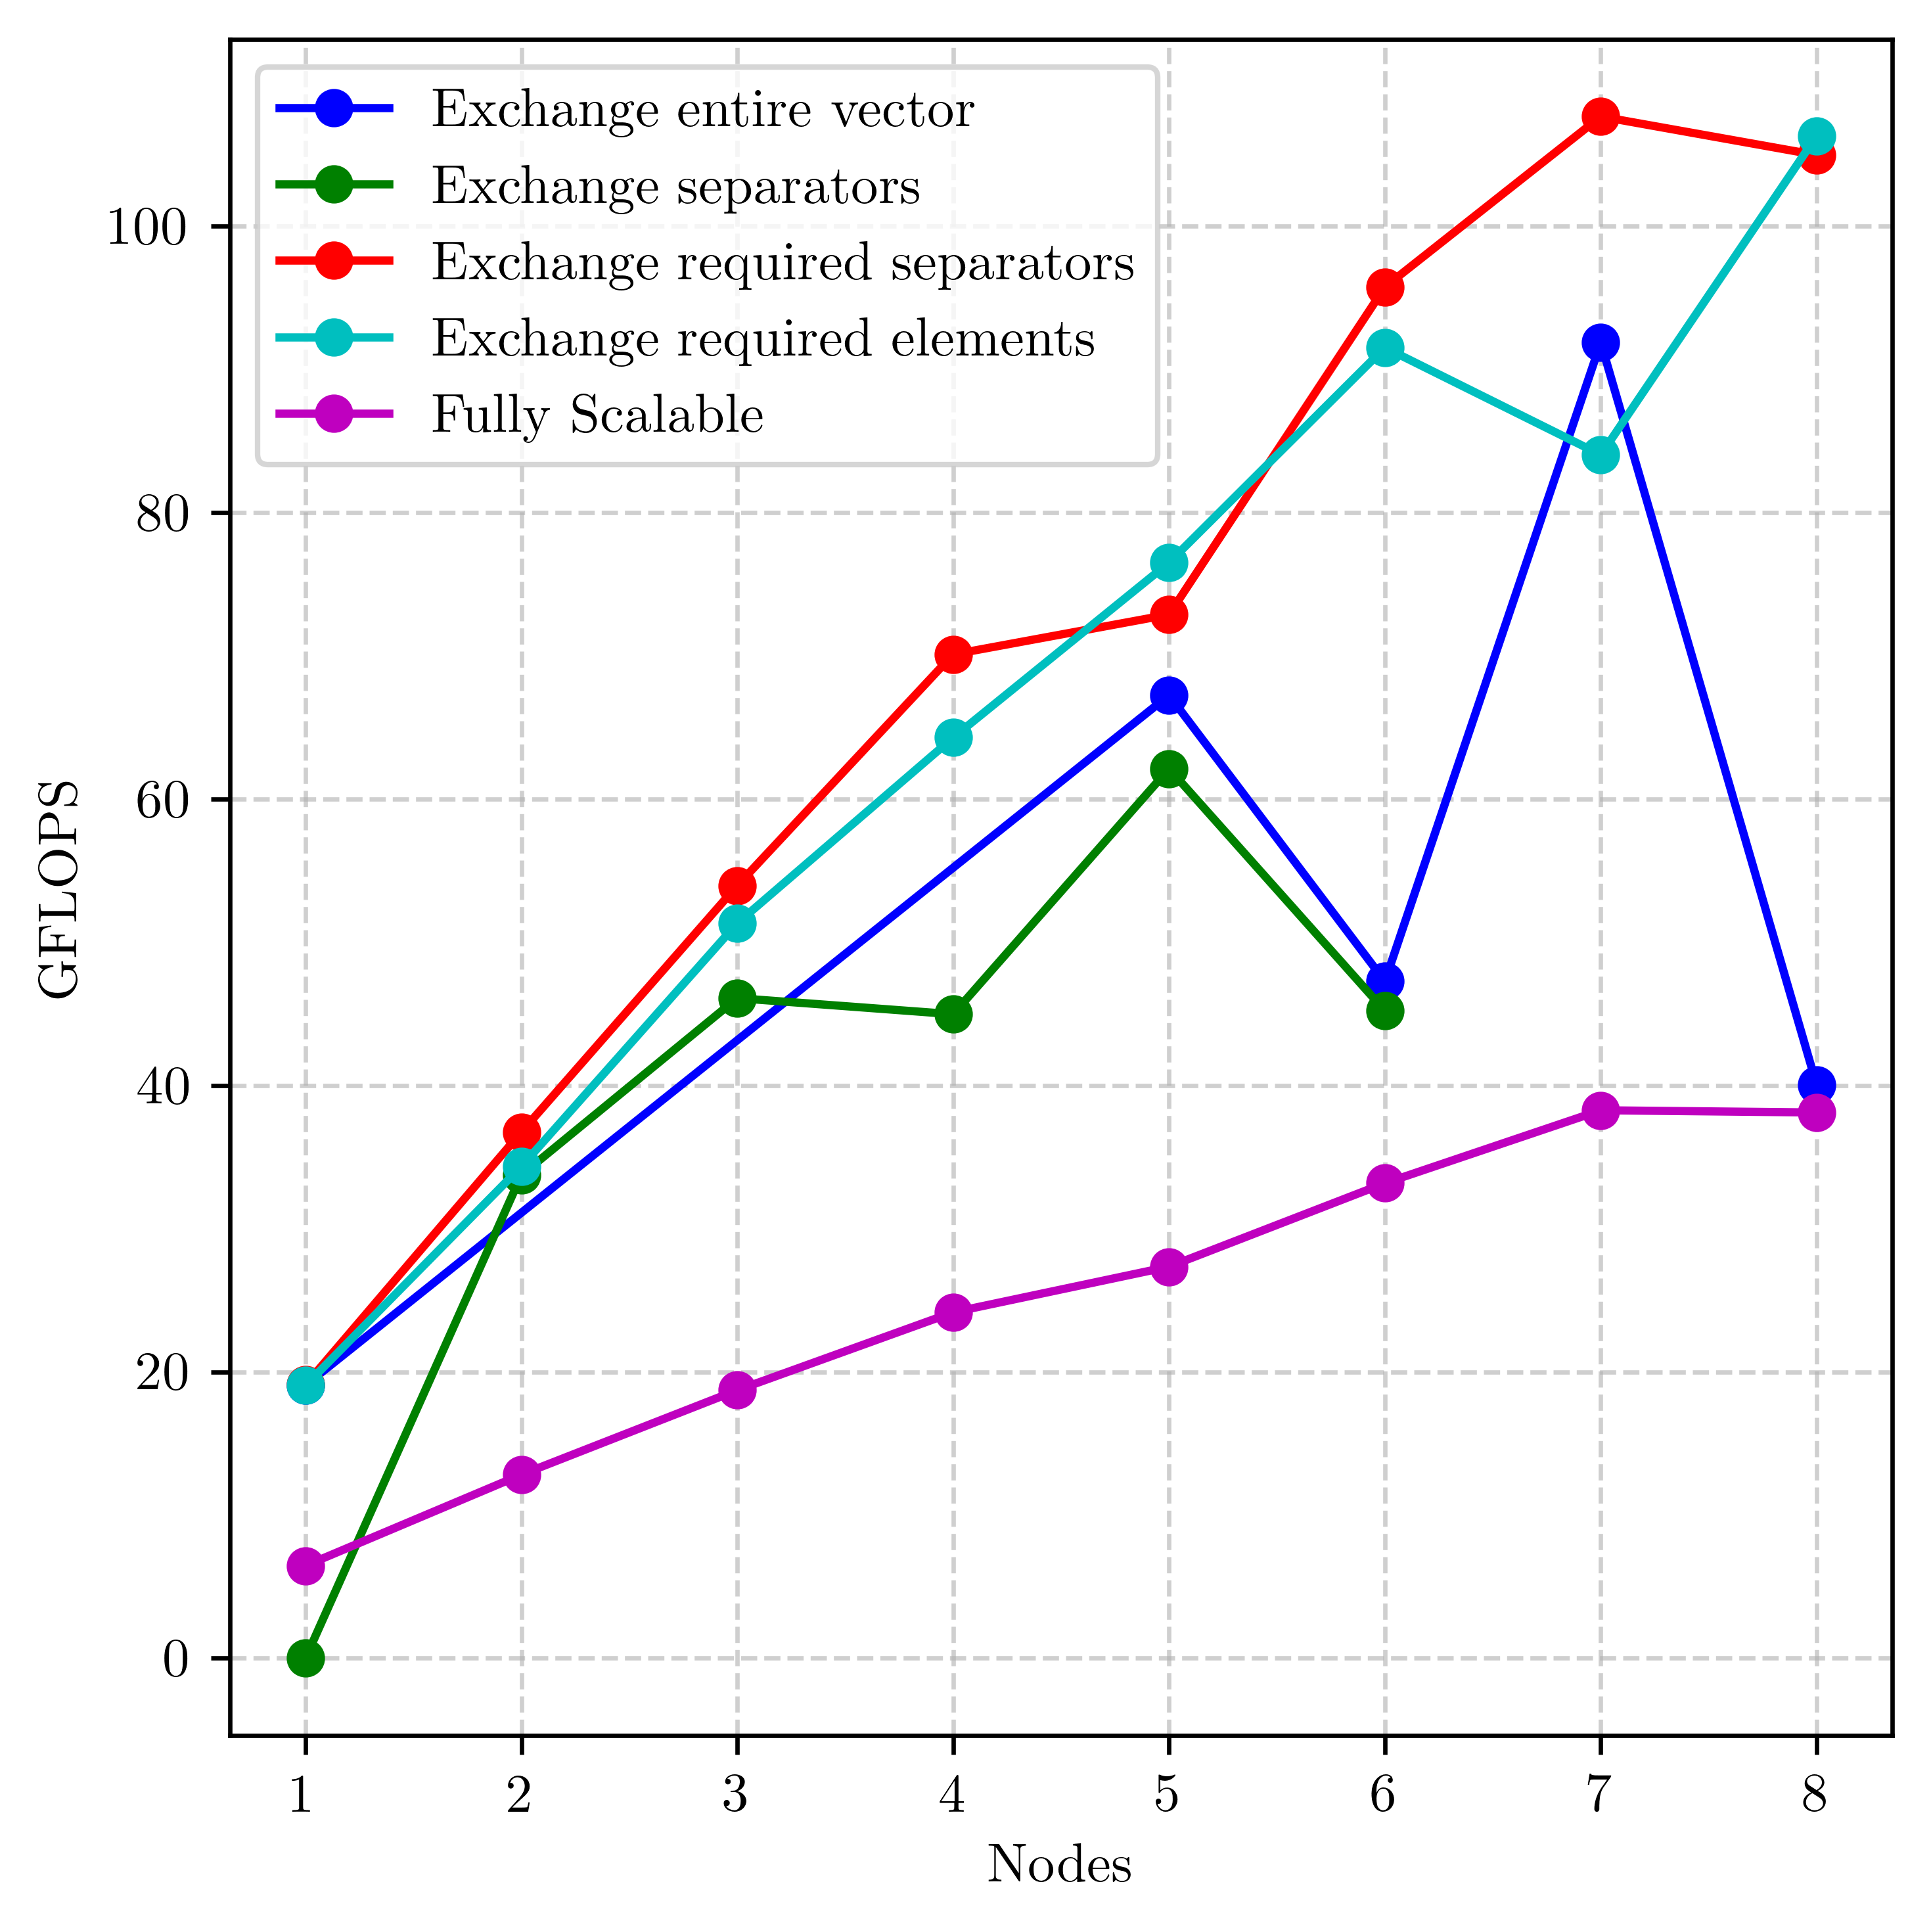
\includegraphics[width=0.95\textwidth]{Cube_Coup_dt0_rome16q}
    \end{center}
    \caption{Cube\_Coup\_dt0}
    \label{fig:Cube_Coup_dt0_rome16q}
\end{figure}

\begin{figure}[H]
    \begin{center}
        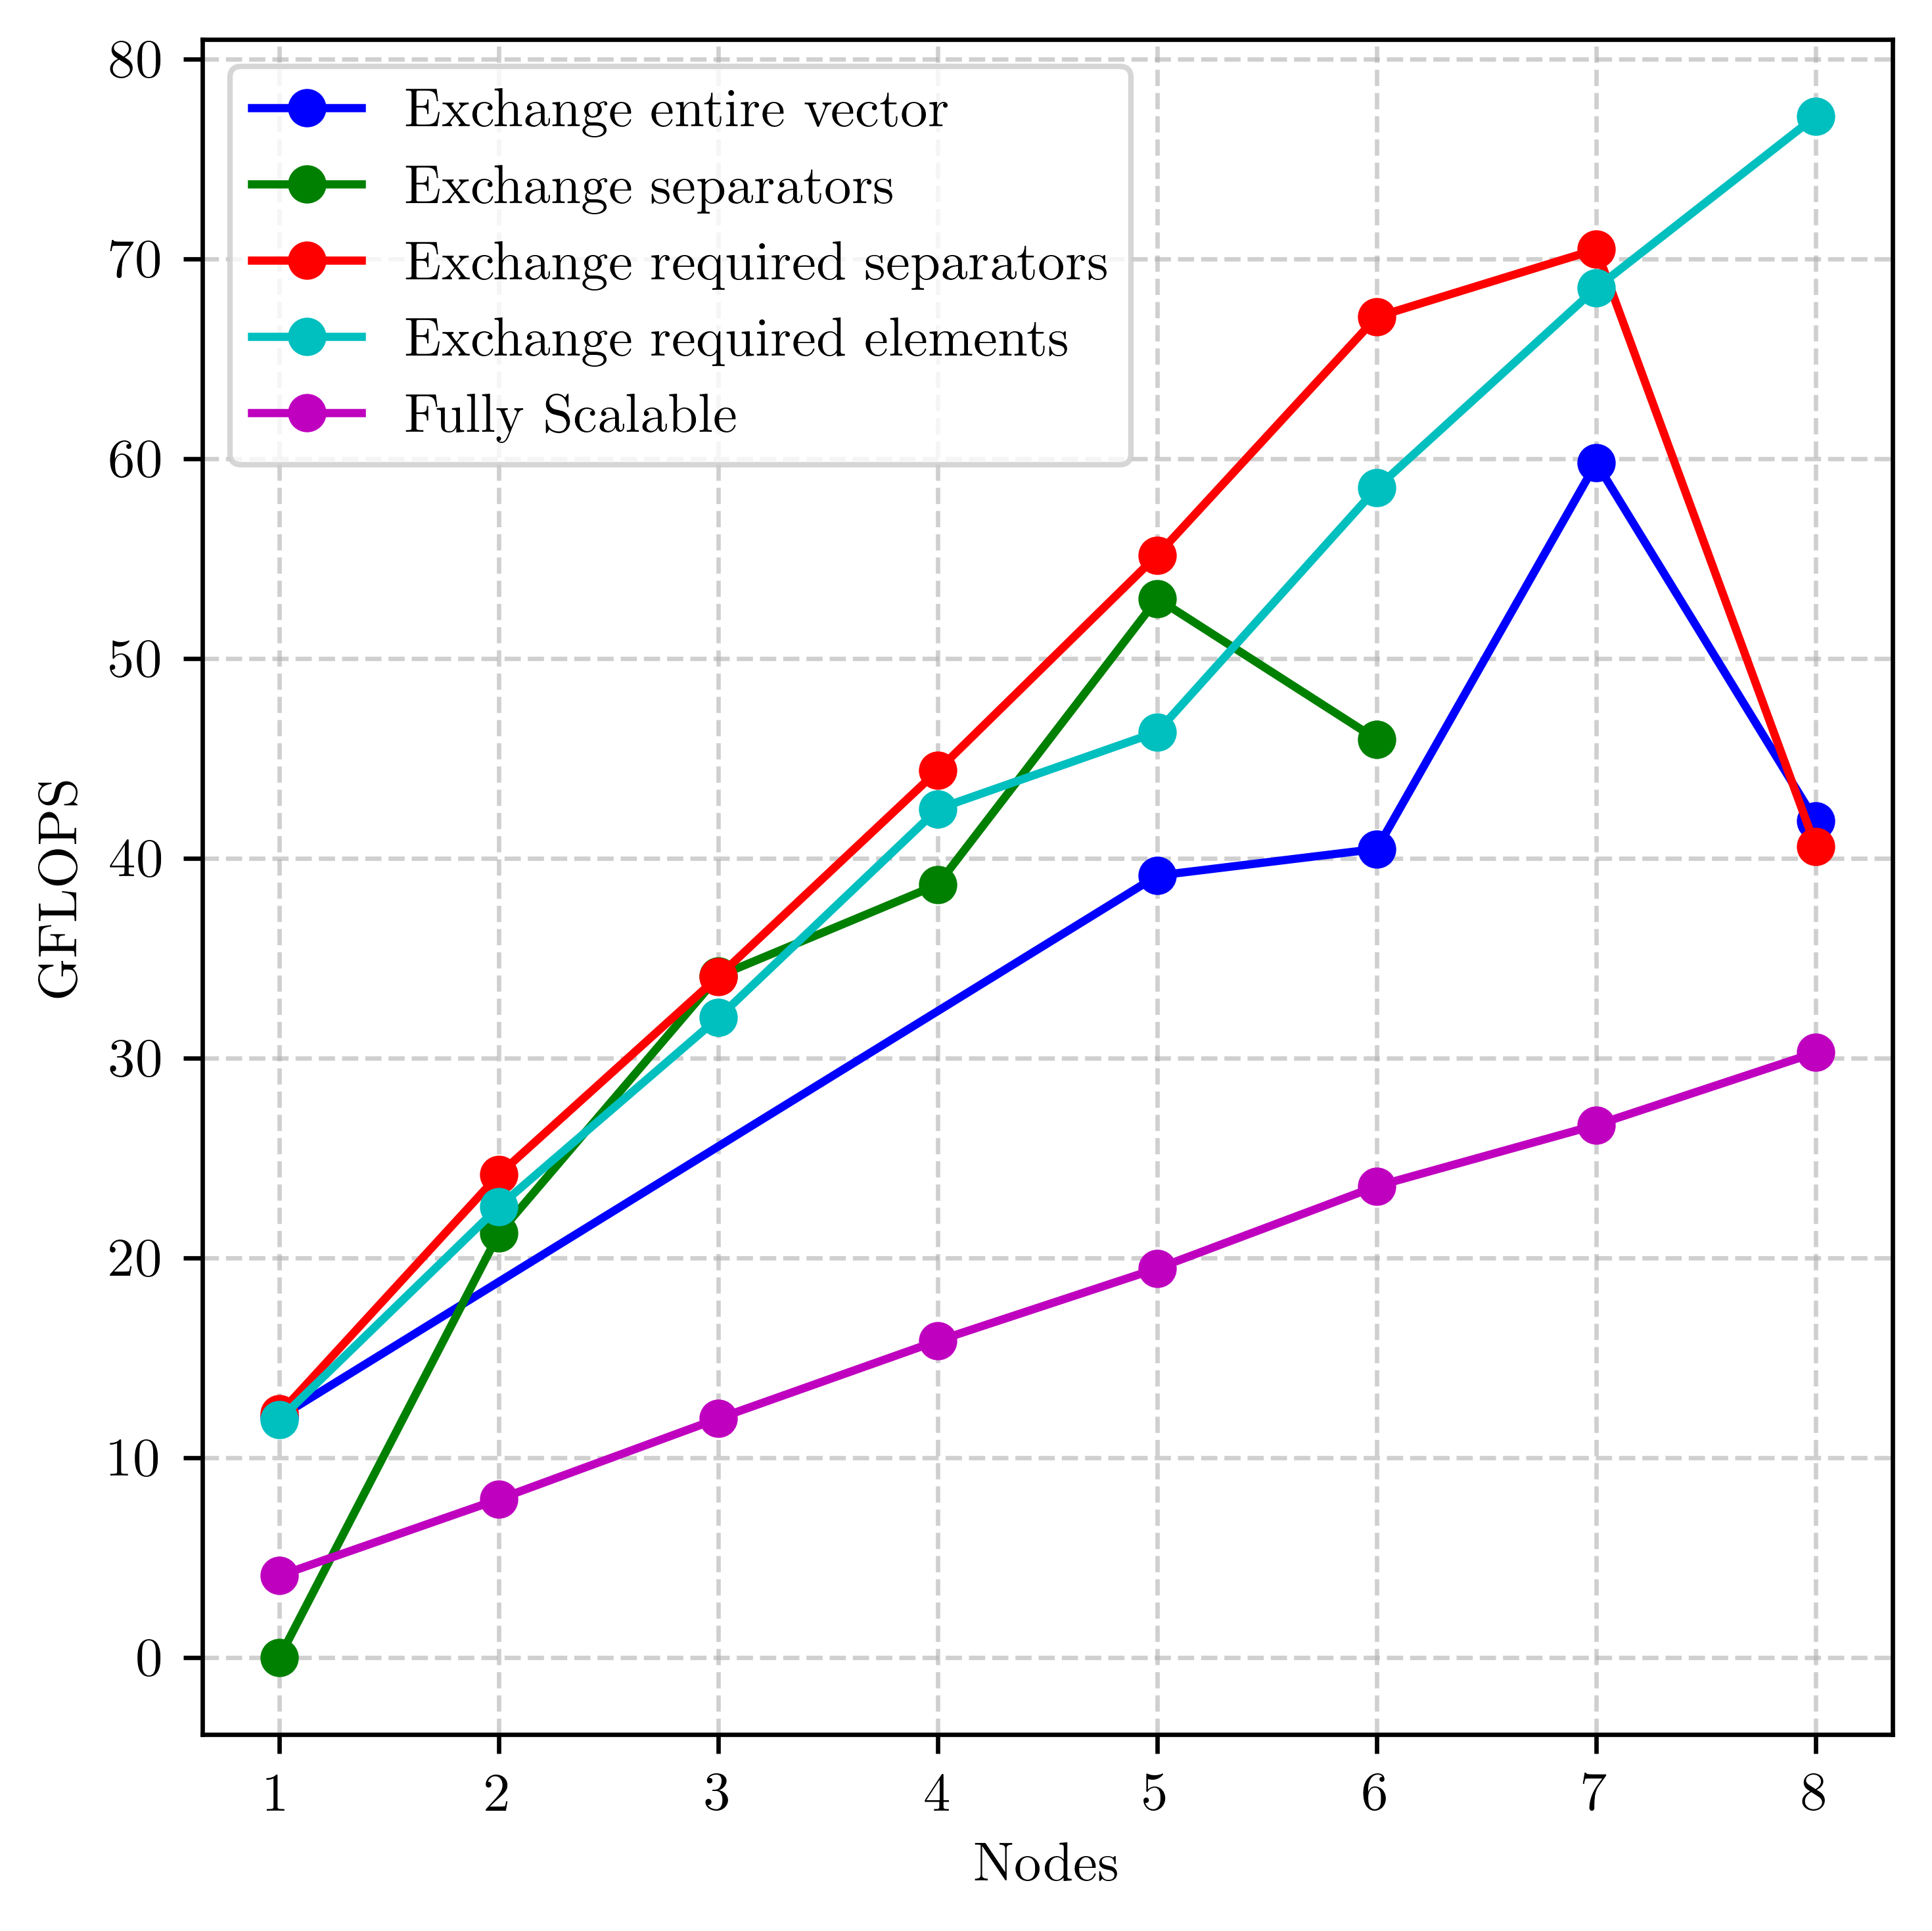
\includegraphics[width=0.95\textwidth]{dielFilterV3real_rome16q}
    \end{center}
    \caption{dielFilterV3real}
    \label{fig:dielFilterV3real_rome16q}
\end{figure}

% \section{GFLOPS \fpgaq}


\begin{figure}[H]
    \begin{center}
        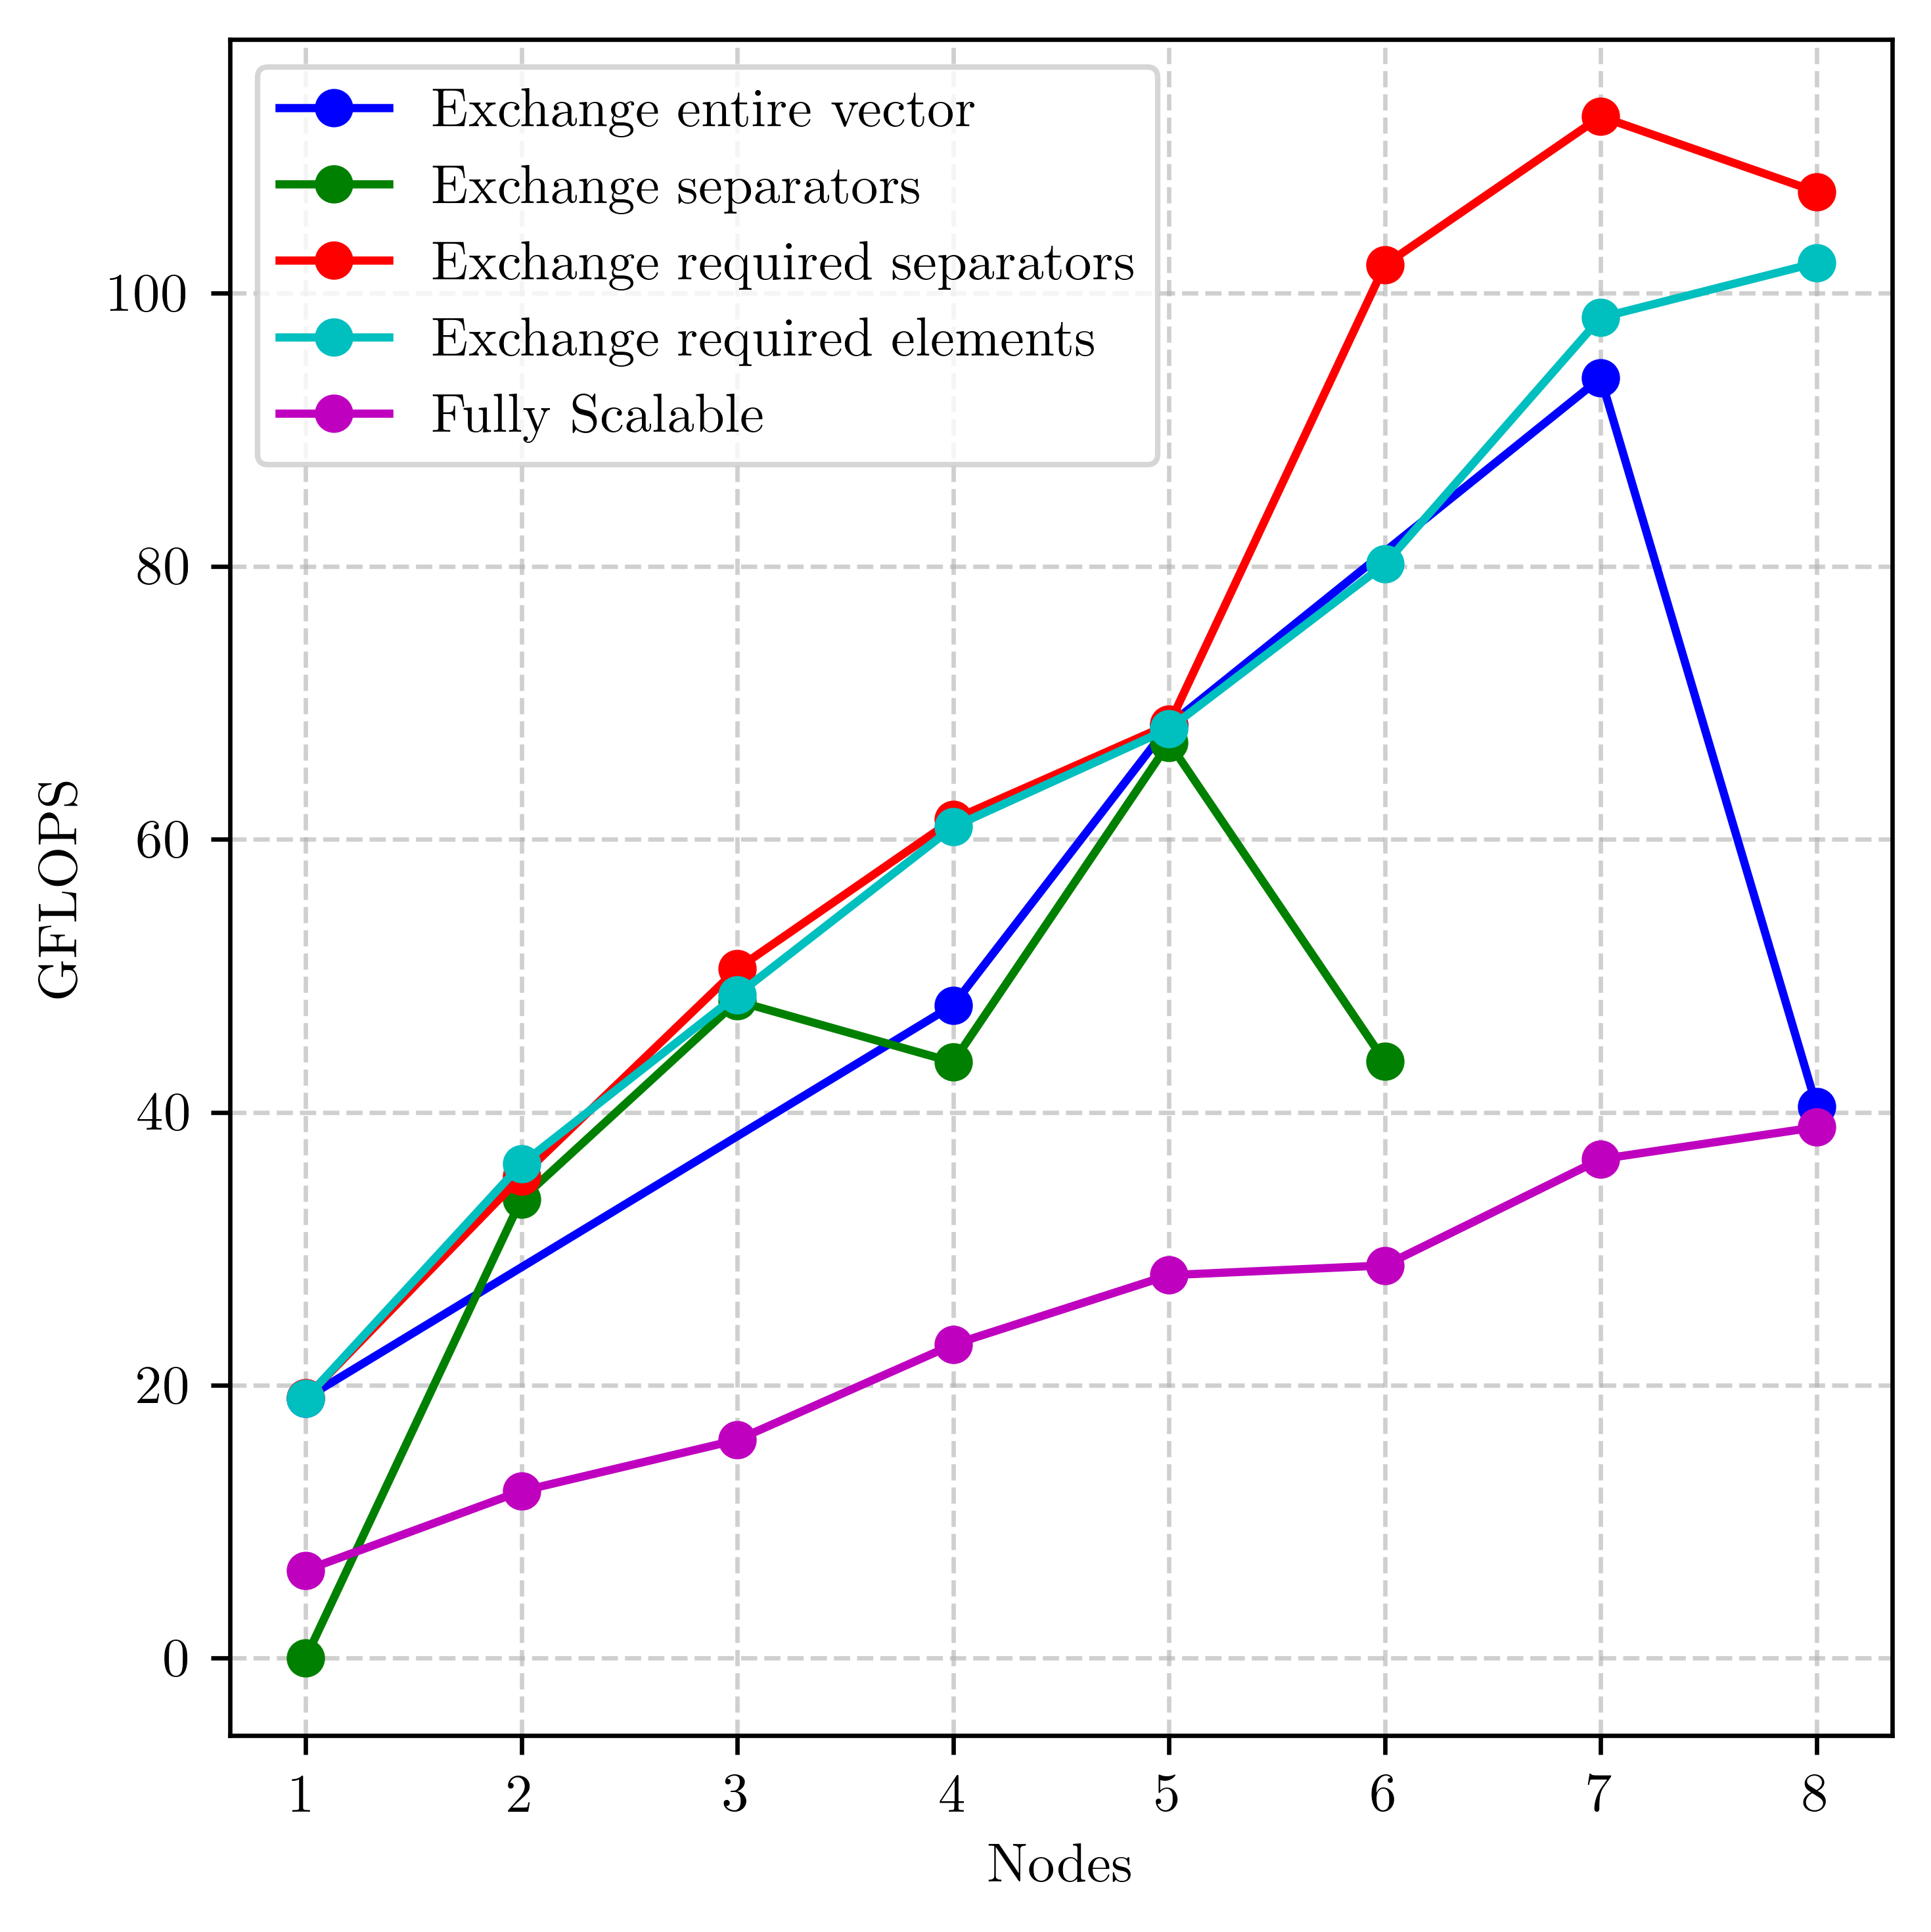
\includegraphics[width=0.95\textwidth]{Long_Coup_dt0_rome16q}
    \end{center}
    \caption{Long\_Coup\_dt0}
    \label{fig:Long_Coup_dt0_rome16q}
\end{figure}

\begin{figure}[H]
    \begin{center}
        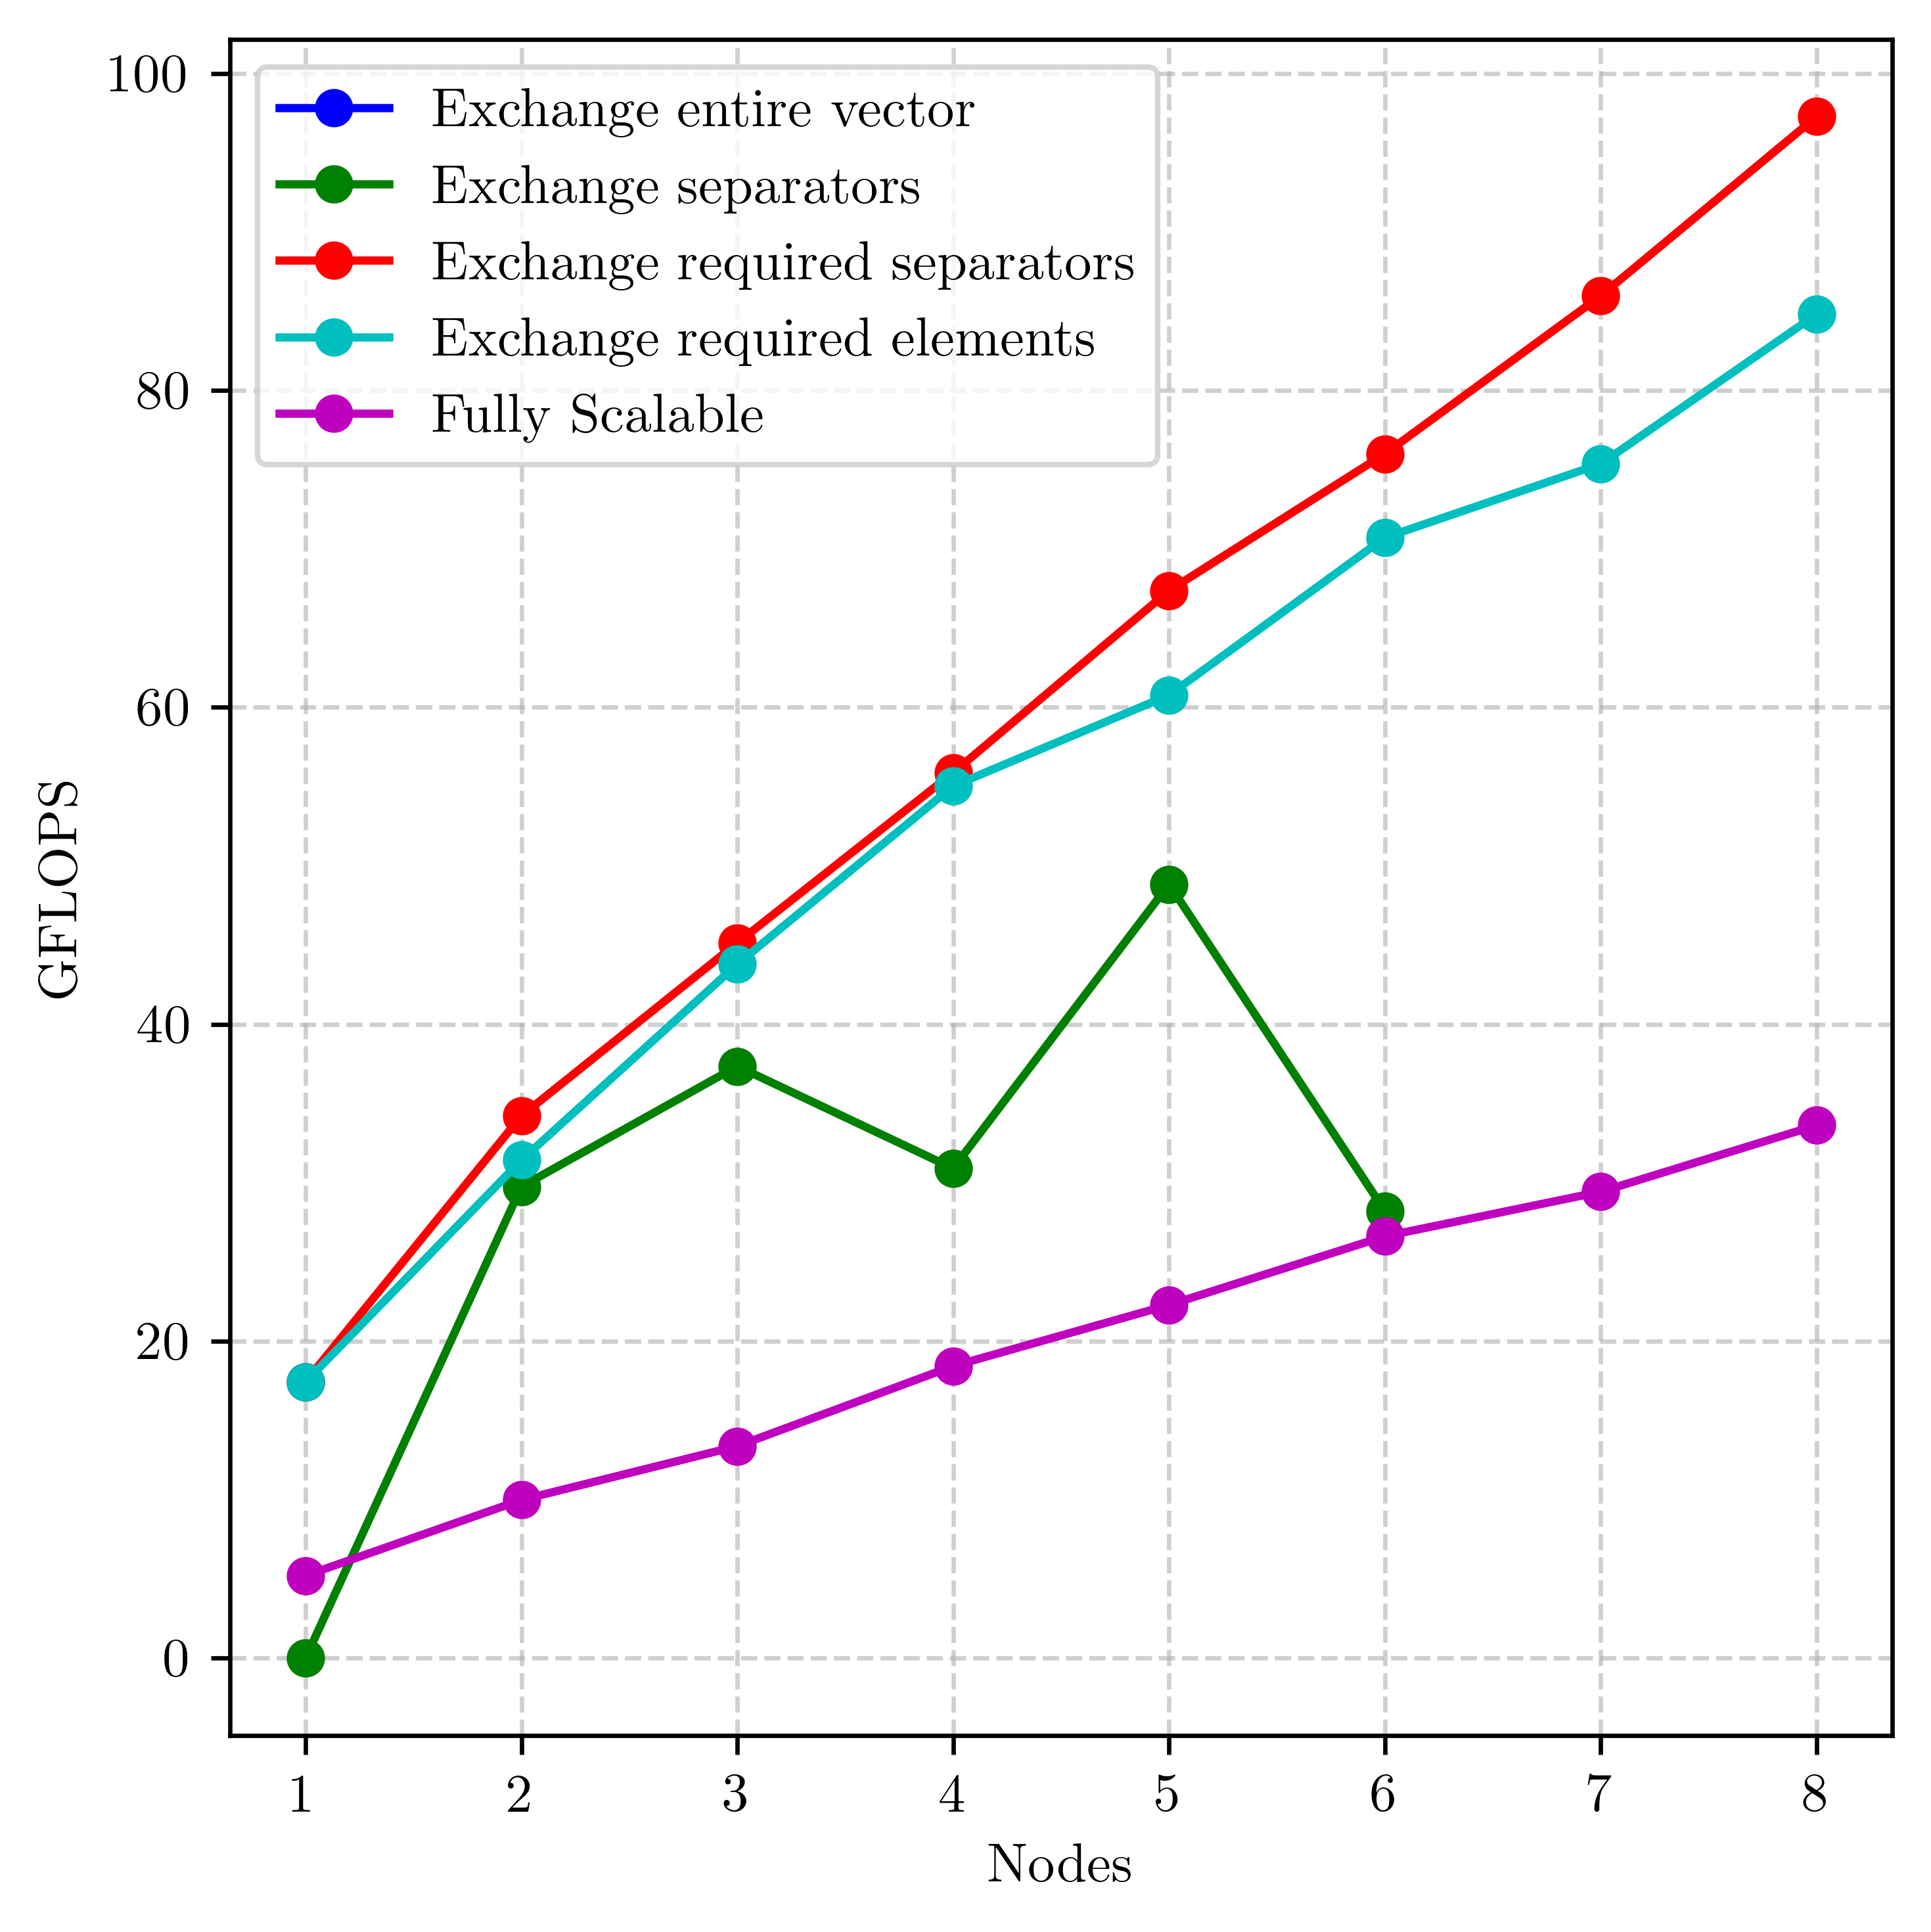
\includegraphics[width=0.95\textwidth]{nlpkkt200_rome16q}
    \end{center}
    \caption{nlpkkt200}
    \label{fig:nlpkkt200_rome16q}
\end{figure}




\section{GFLOPS \fpgaq}

\begin{figure}[H]
    \begin{center}
        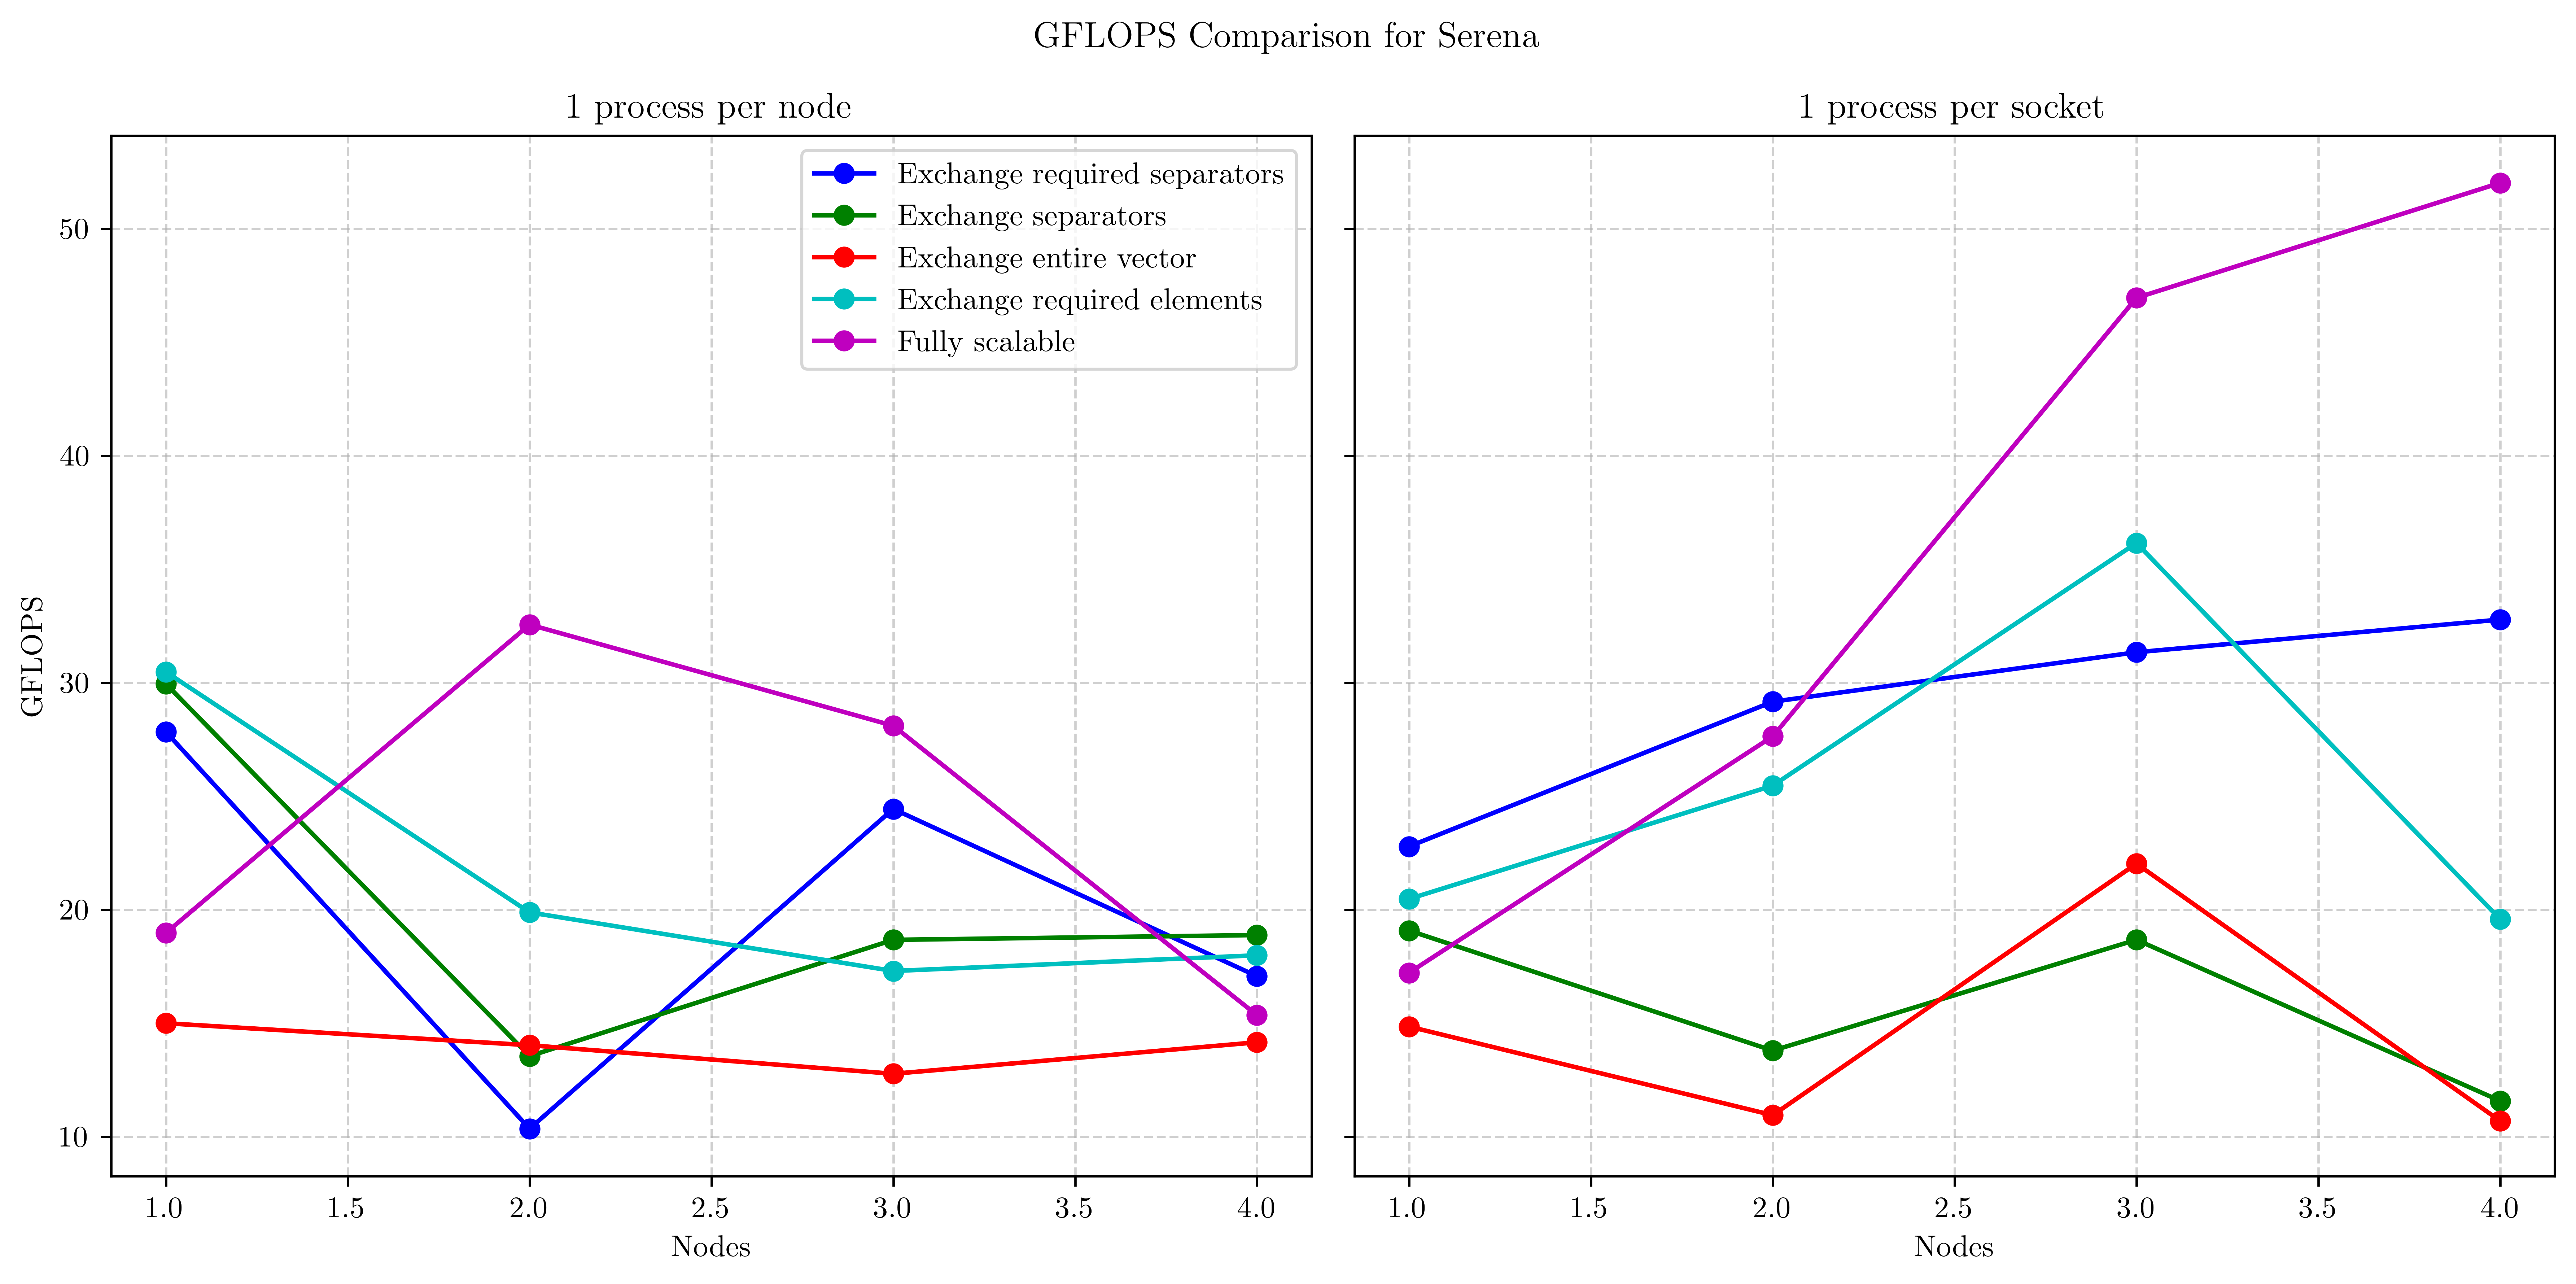
\includegraphics[width=0.95\textwidth]{Serena_fpgaq}
    \end{center}
    \caption{Serena}
    \label{fig:Serena_fpgaq}
\end{figure}

\begin{figure}[H]
    \begin{center}
        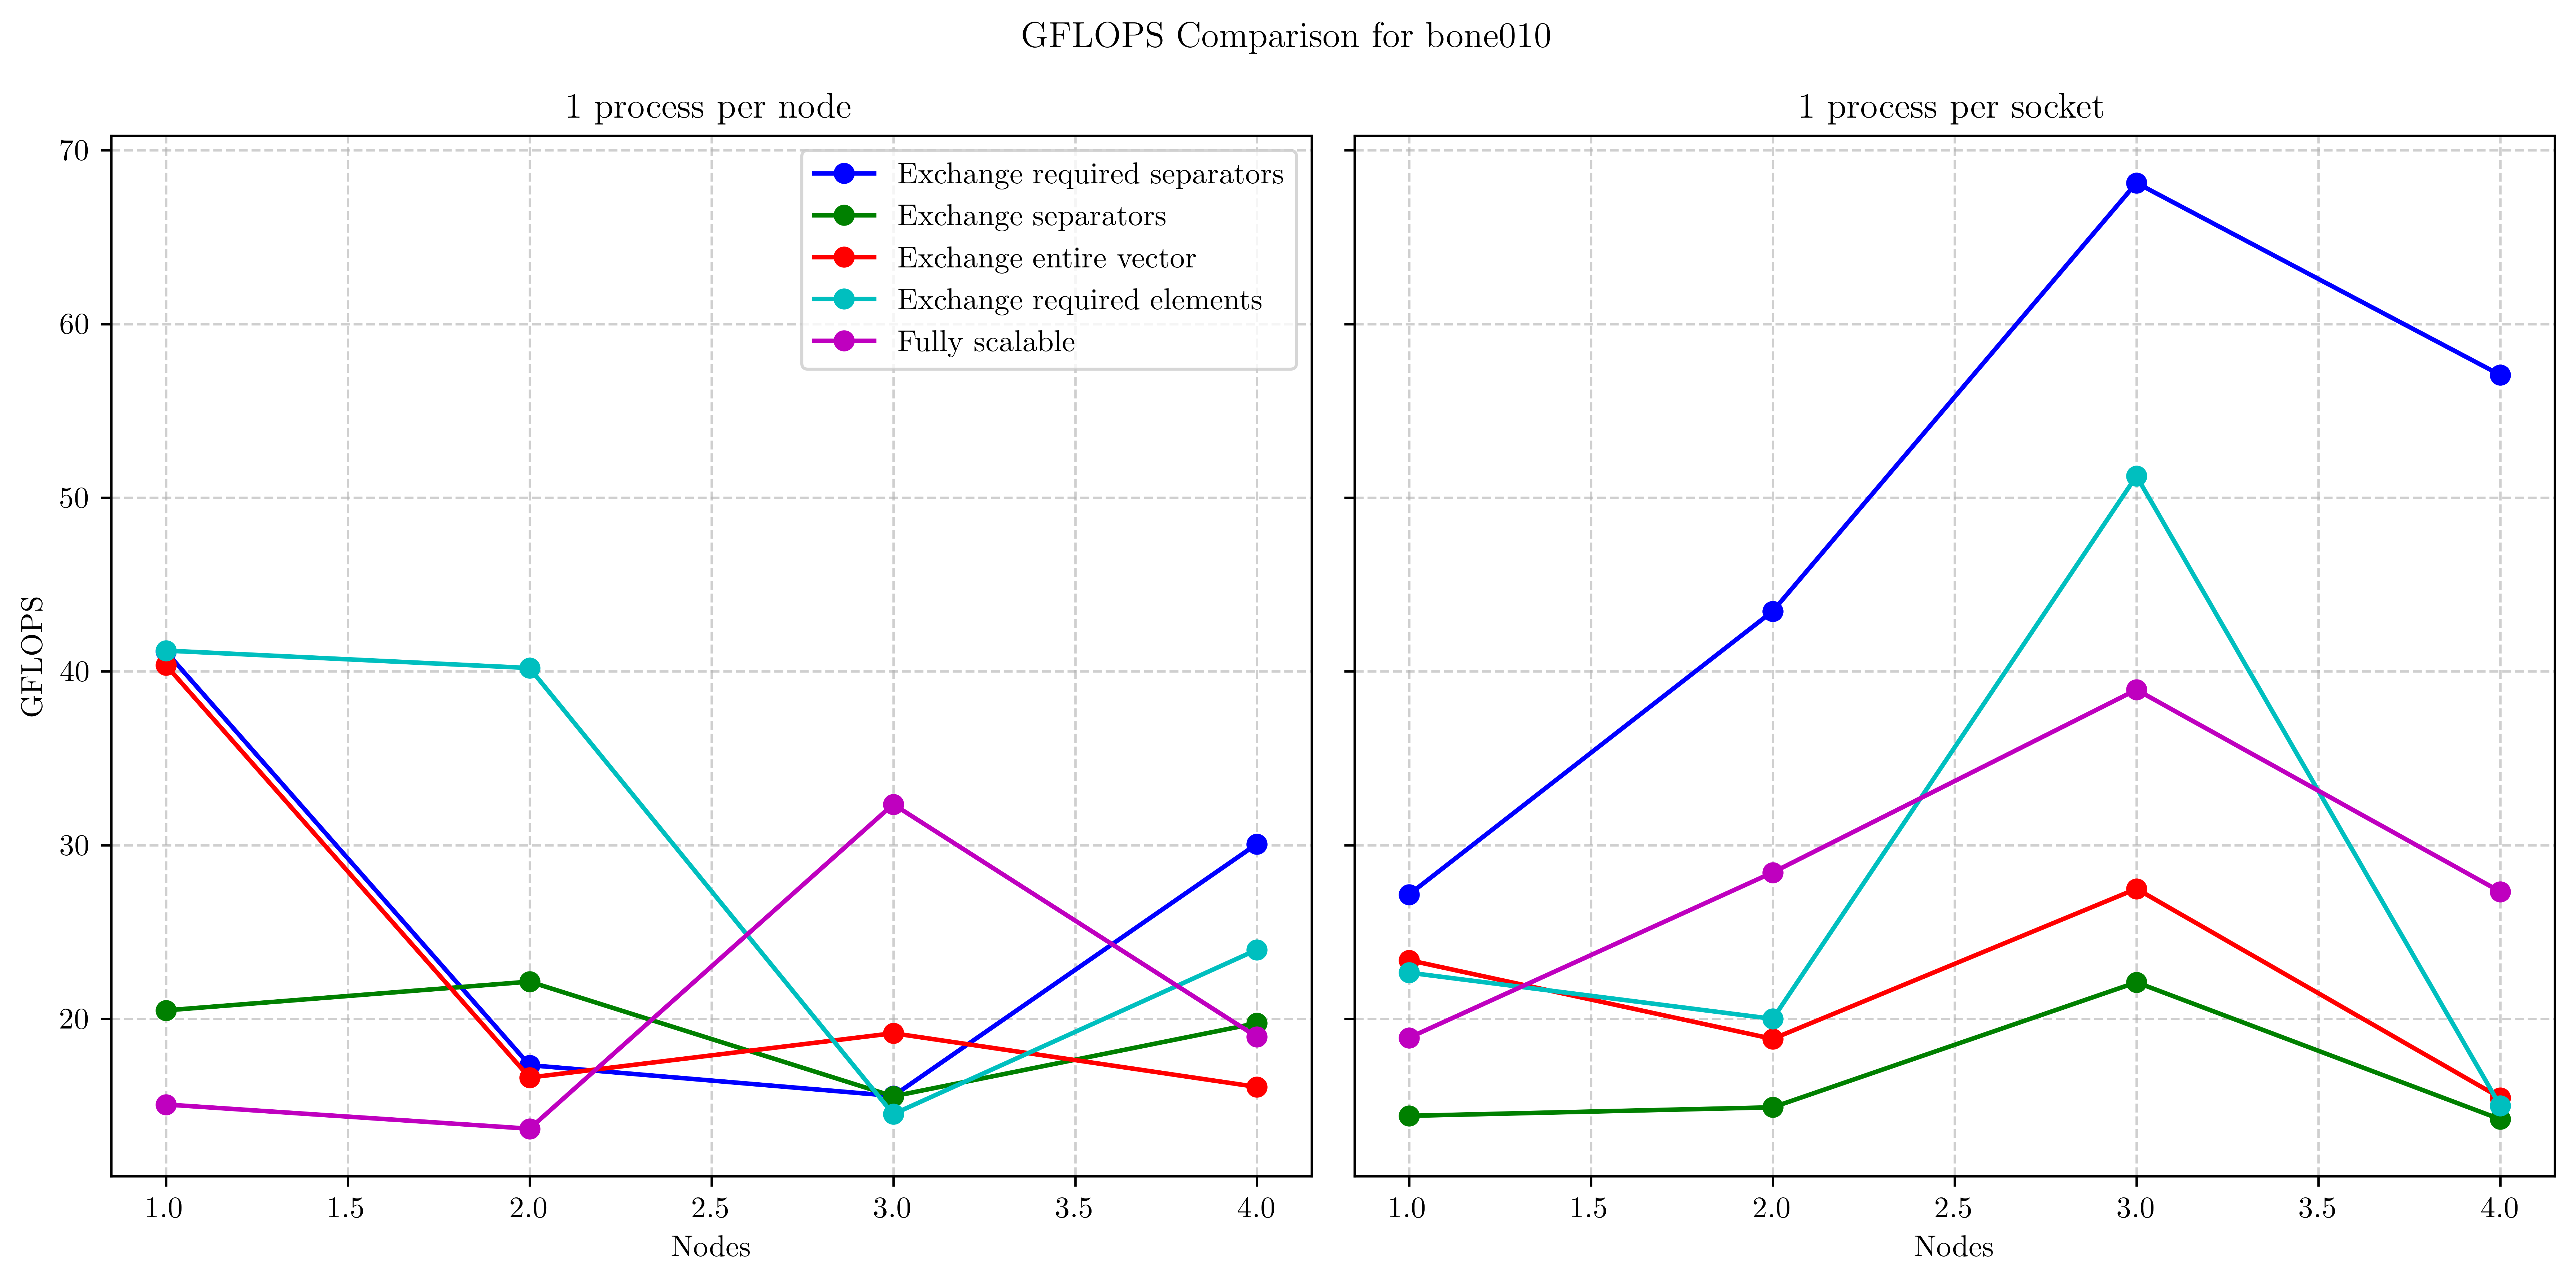
\includegraphics[width=0.95\textwidth]{bone010_fpgaq}
    \end{center}
    \caption{bone010}
    \label{fig:bone010_fpgaq}
\end{figure}

\begin{figure}[H]
    \begin{center}
        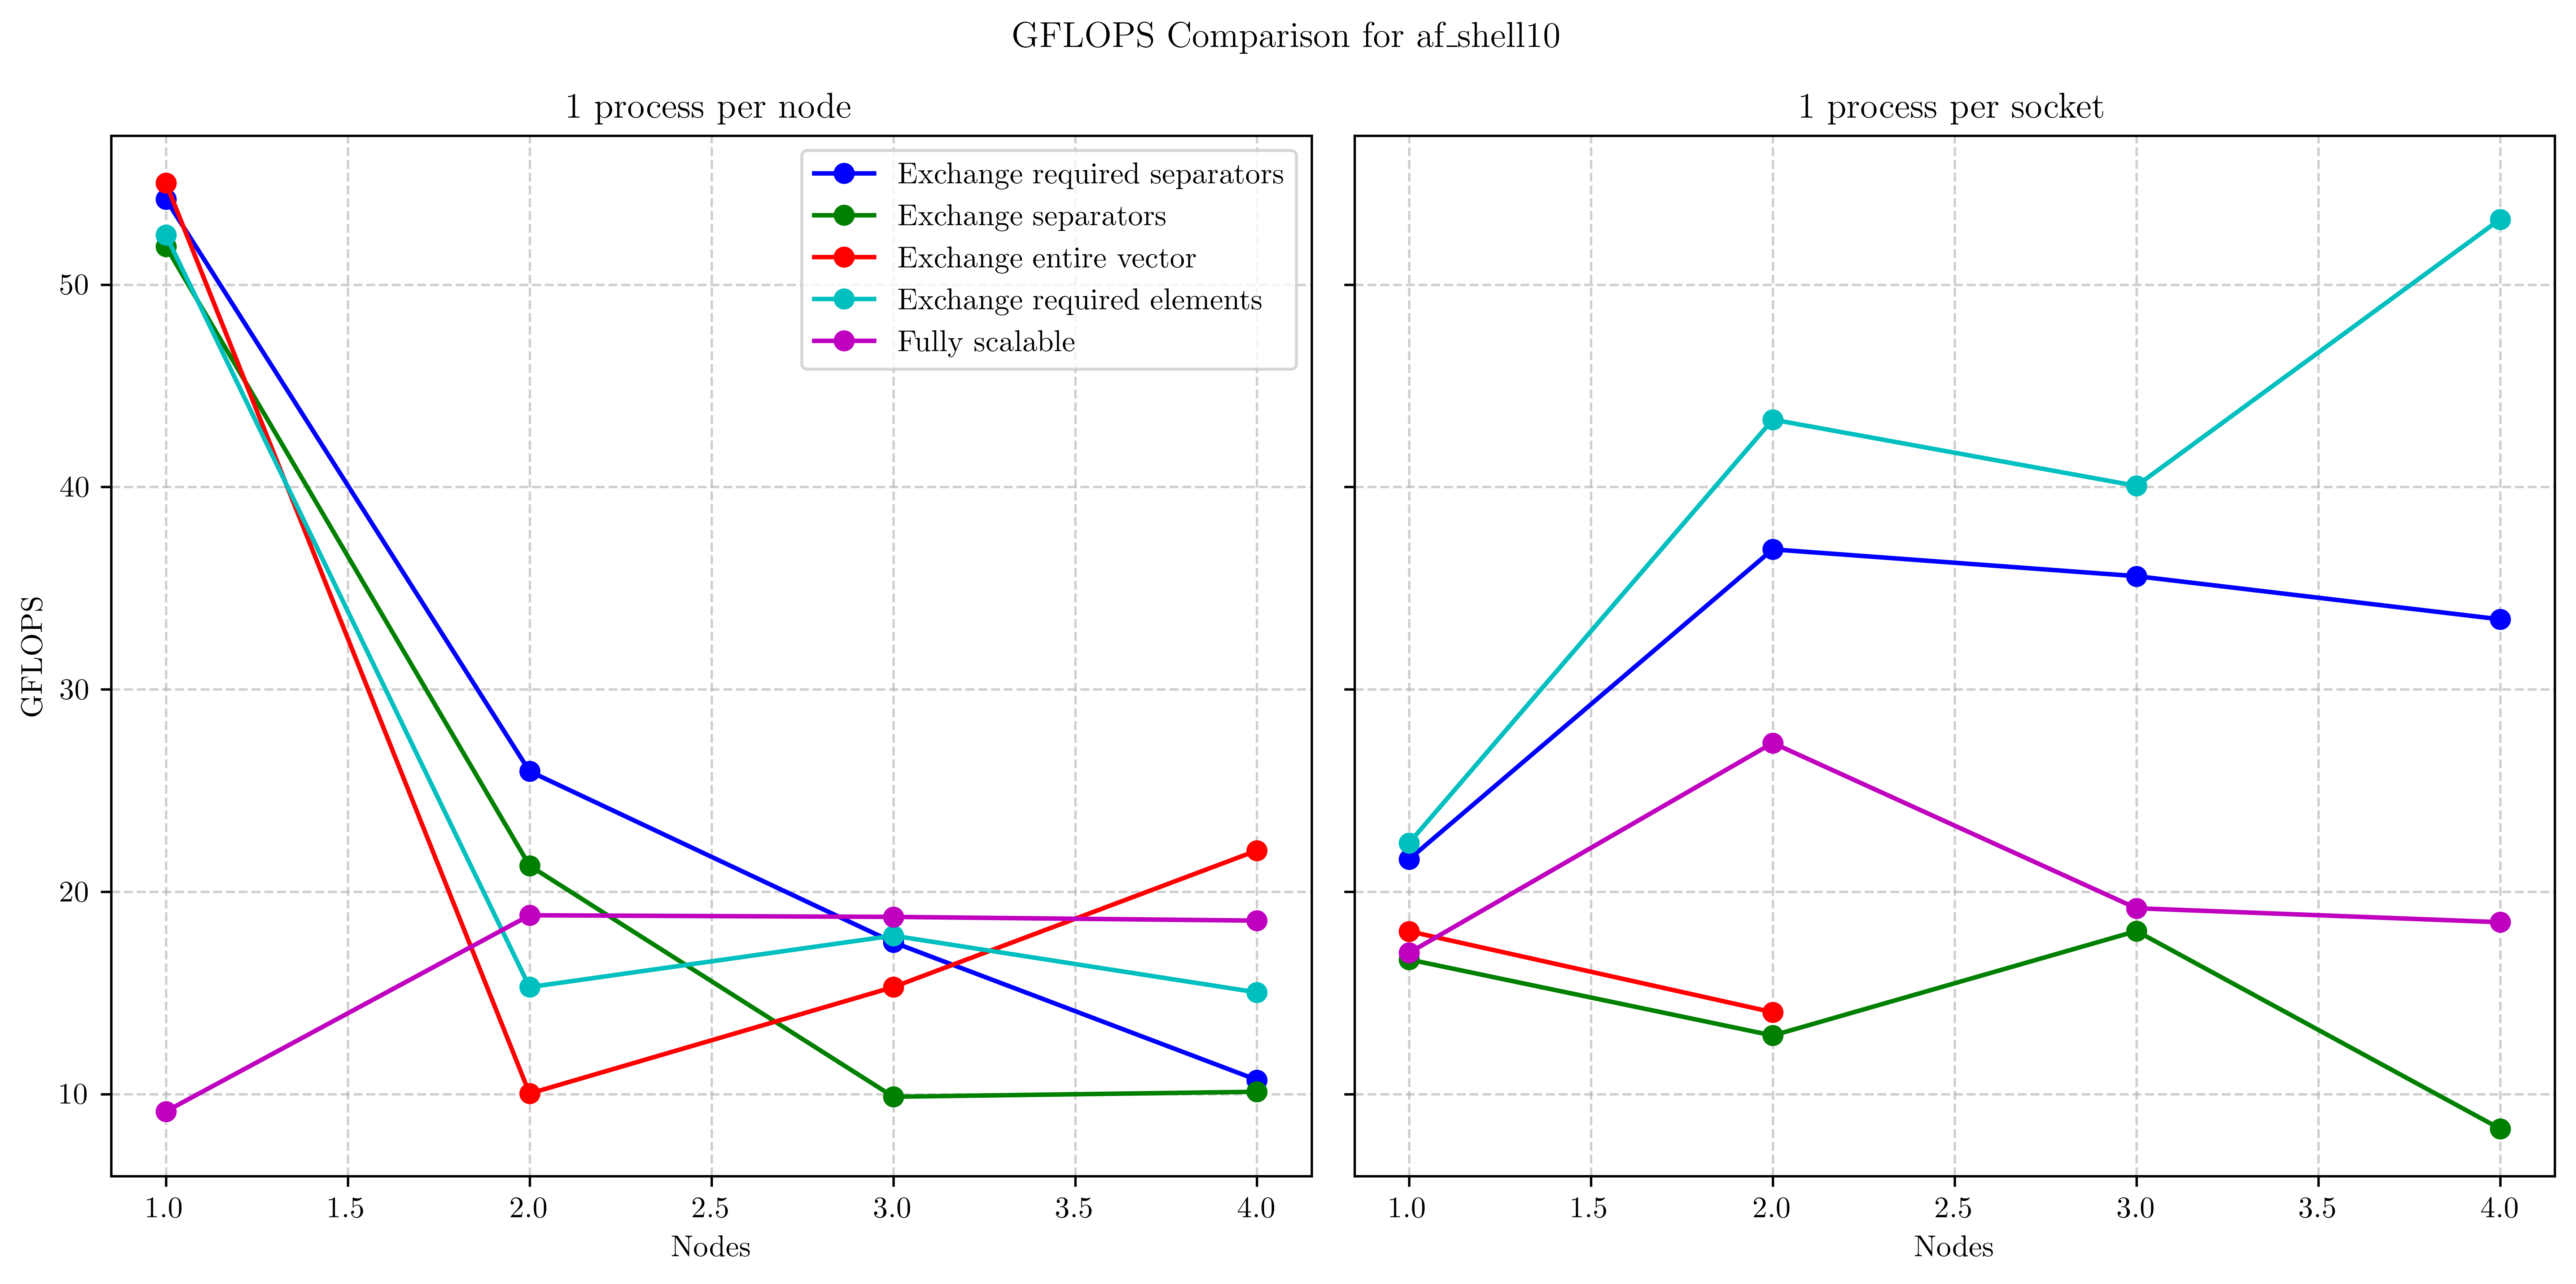
\includegraphics[width=0.95\textwidth]{af_shell10_fpgaq}
    \end{center}
    \caption{af\_shell10}
    \label{fig:af_shell10_fpgaq}
\end{figure}

\begin{figure}[H]
    \begin{center}
        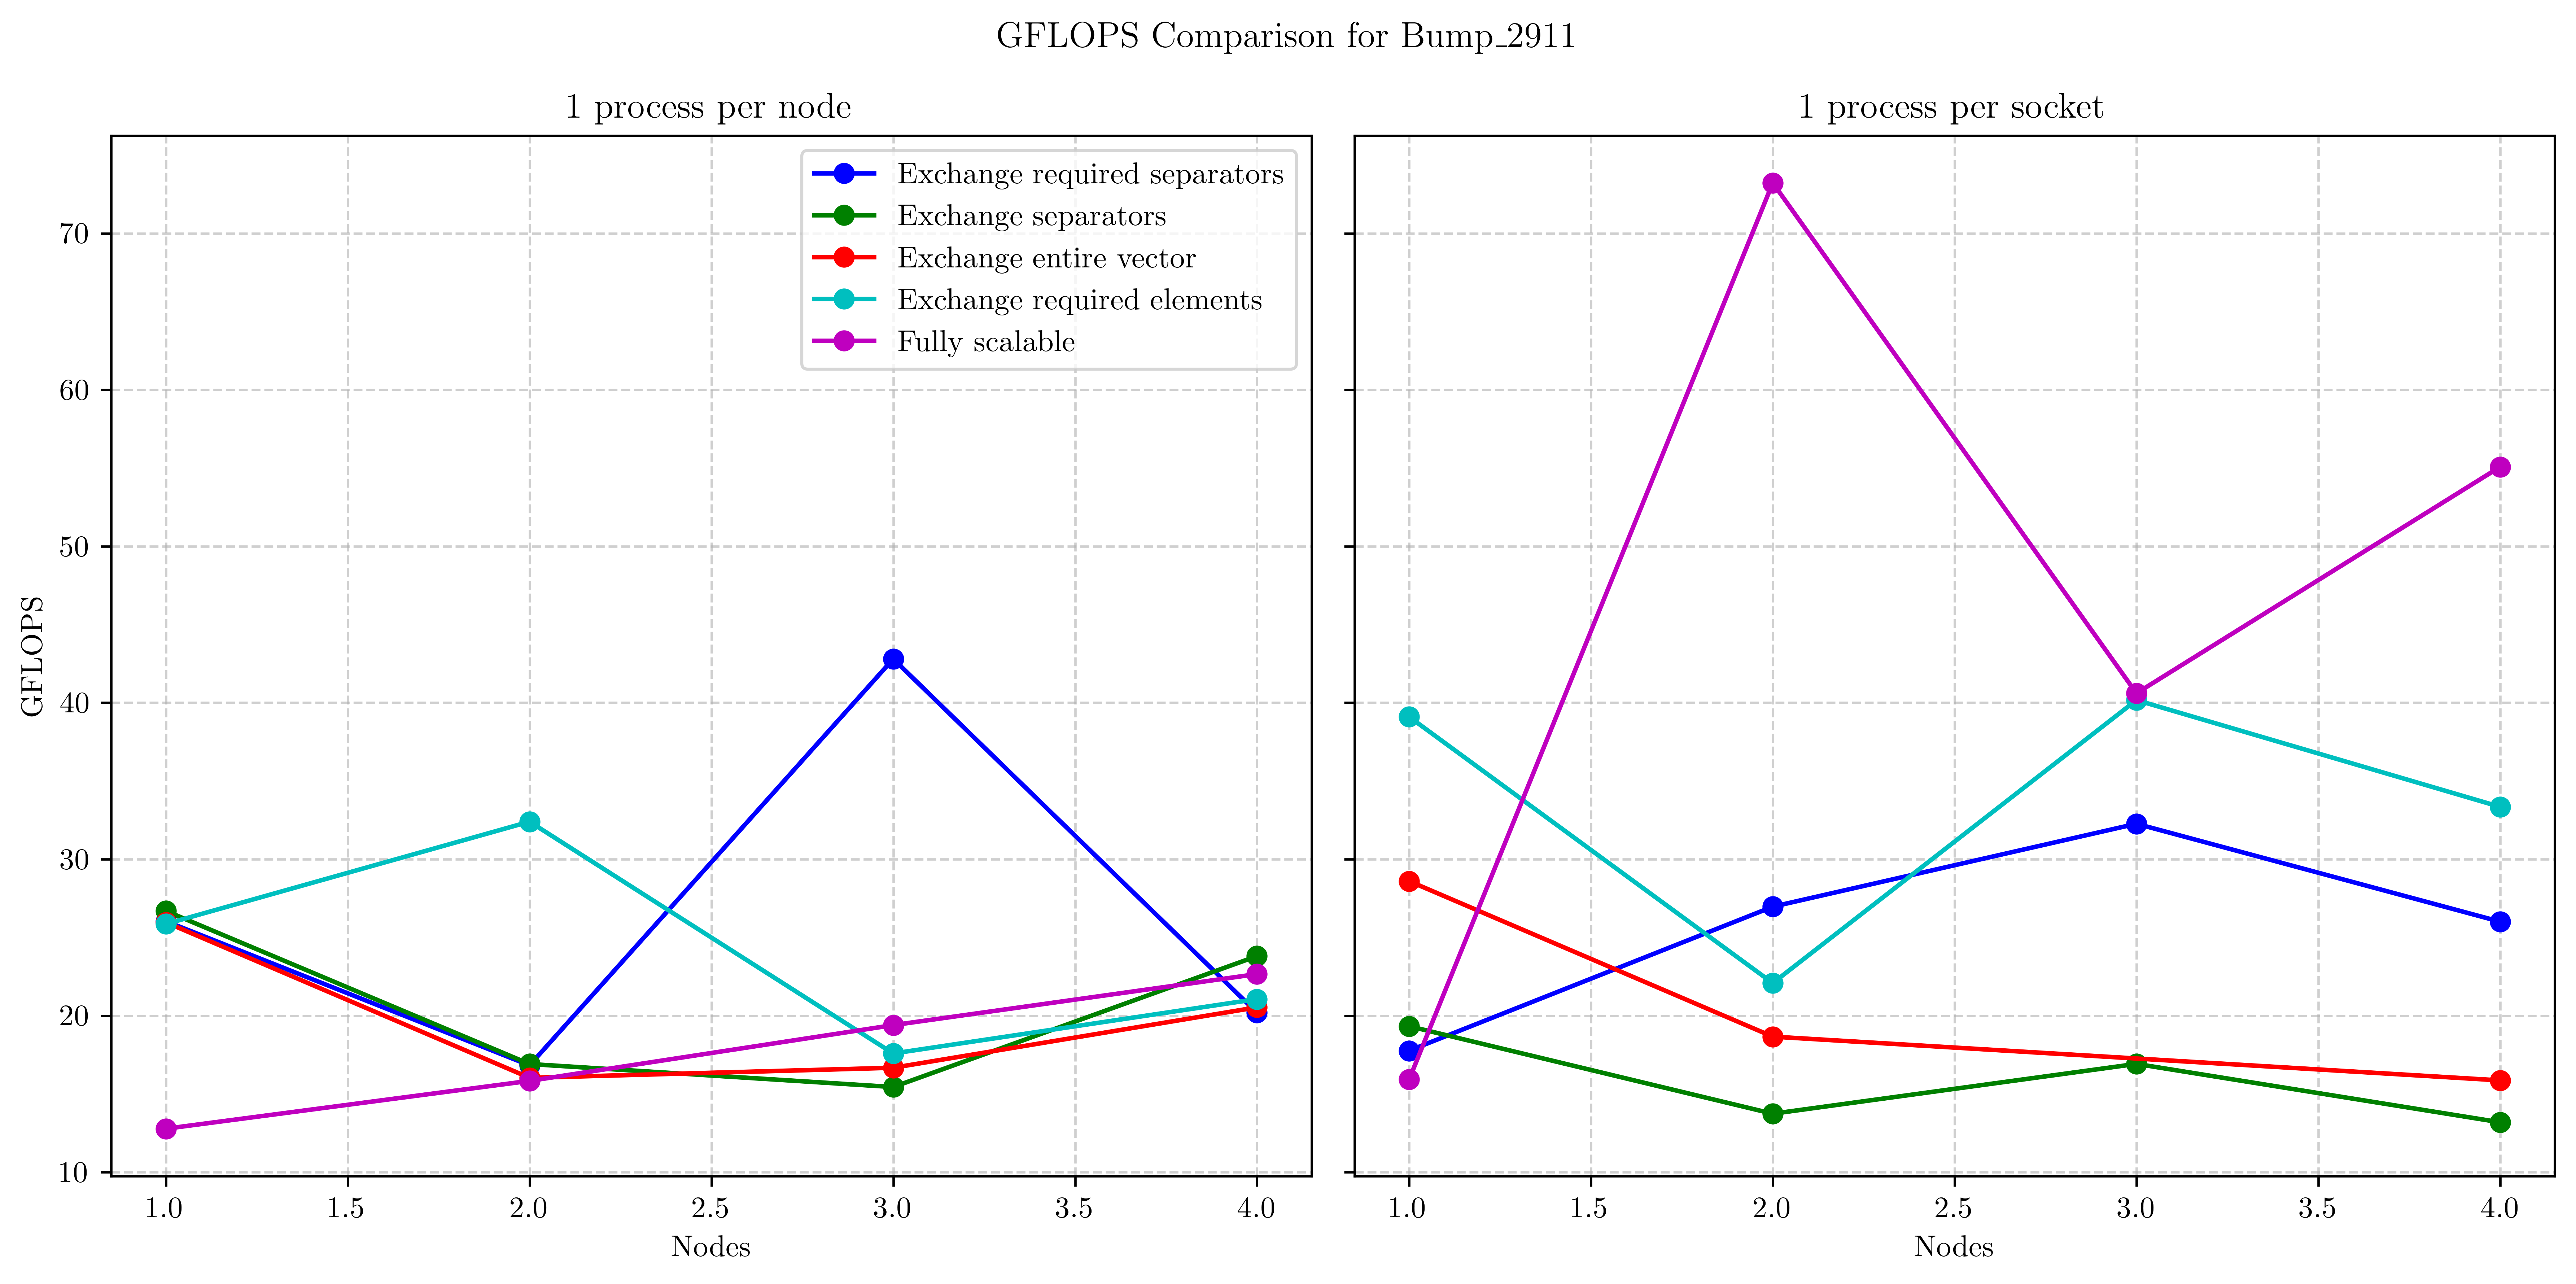
\includegraphics[width=0.95\textwidth]{Bump_2911_fpgaq}
    \end{center}
    \caption{Bump\_2911}
    \label{fig:Bump_2911_fpgaq}
\end{figure}

\begin{figure}[H]
    \begin{center}
        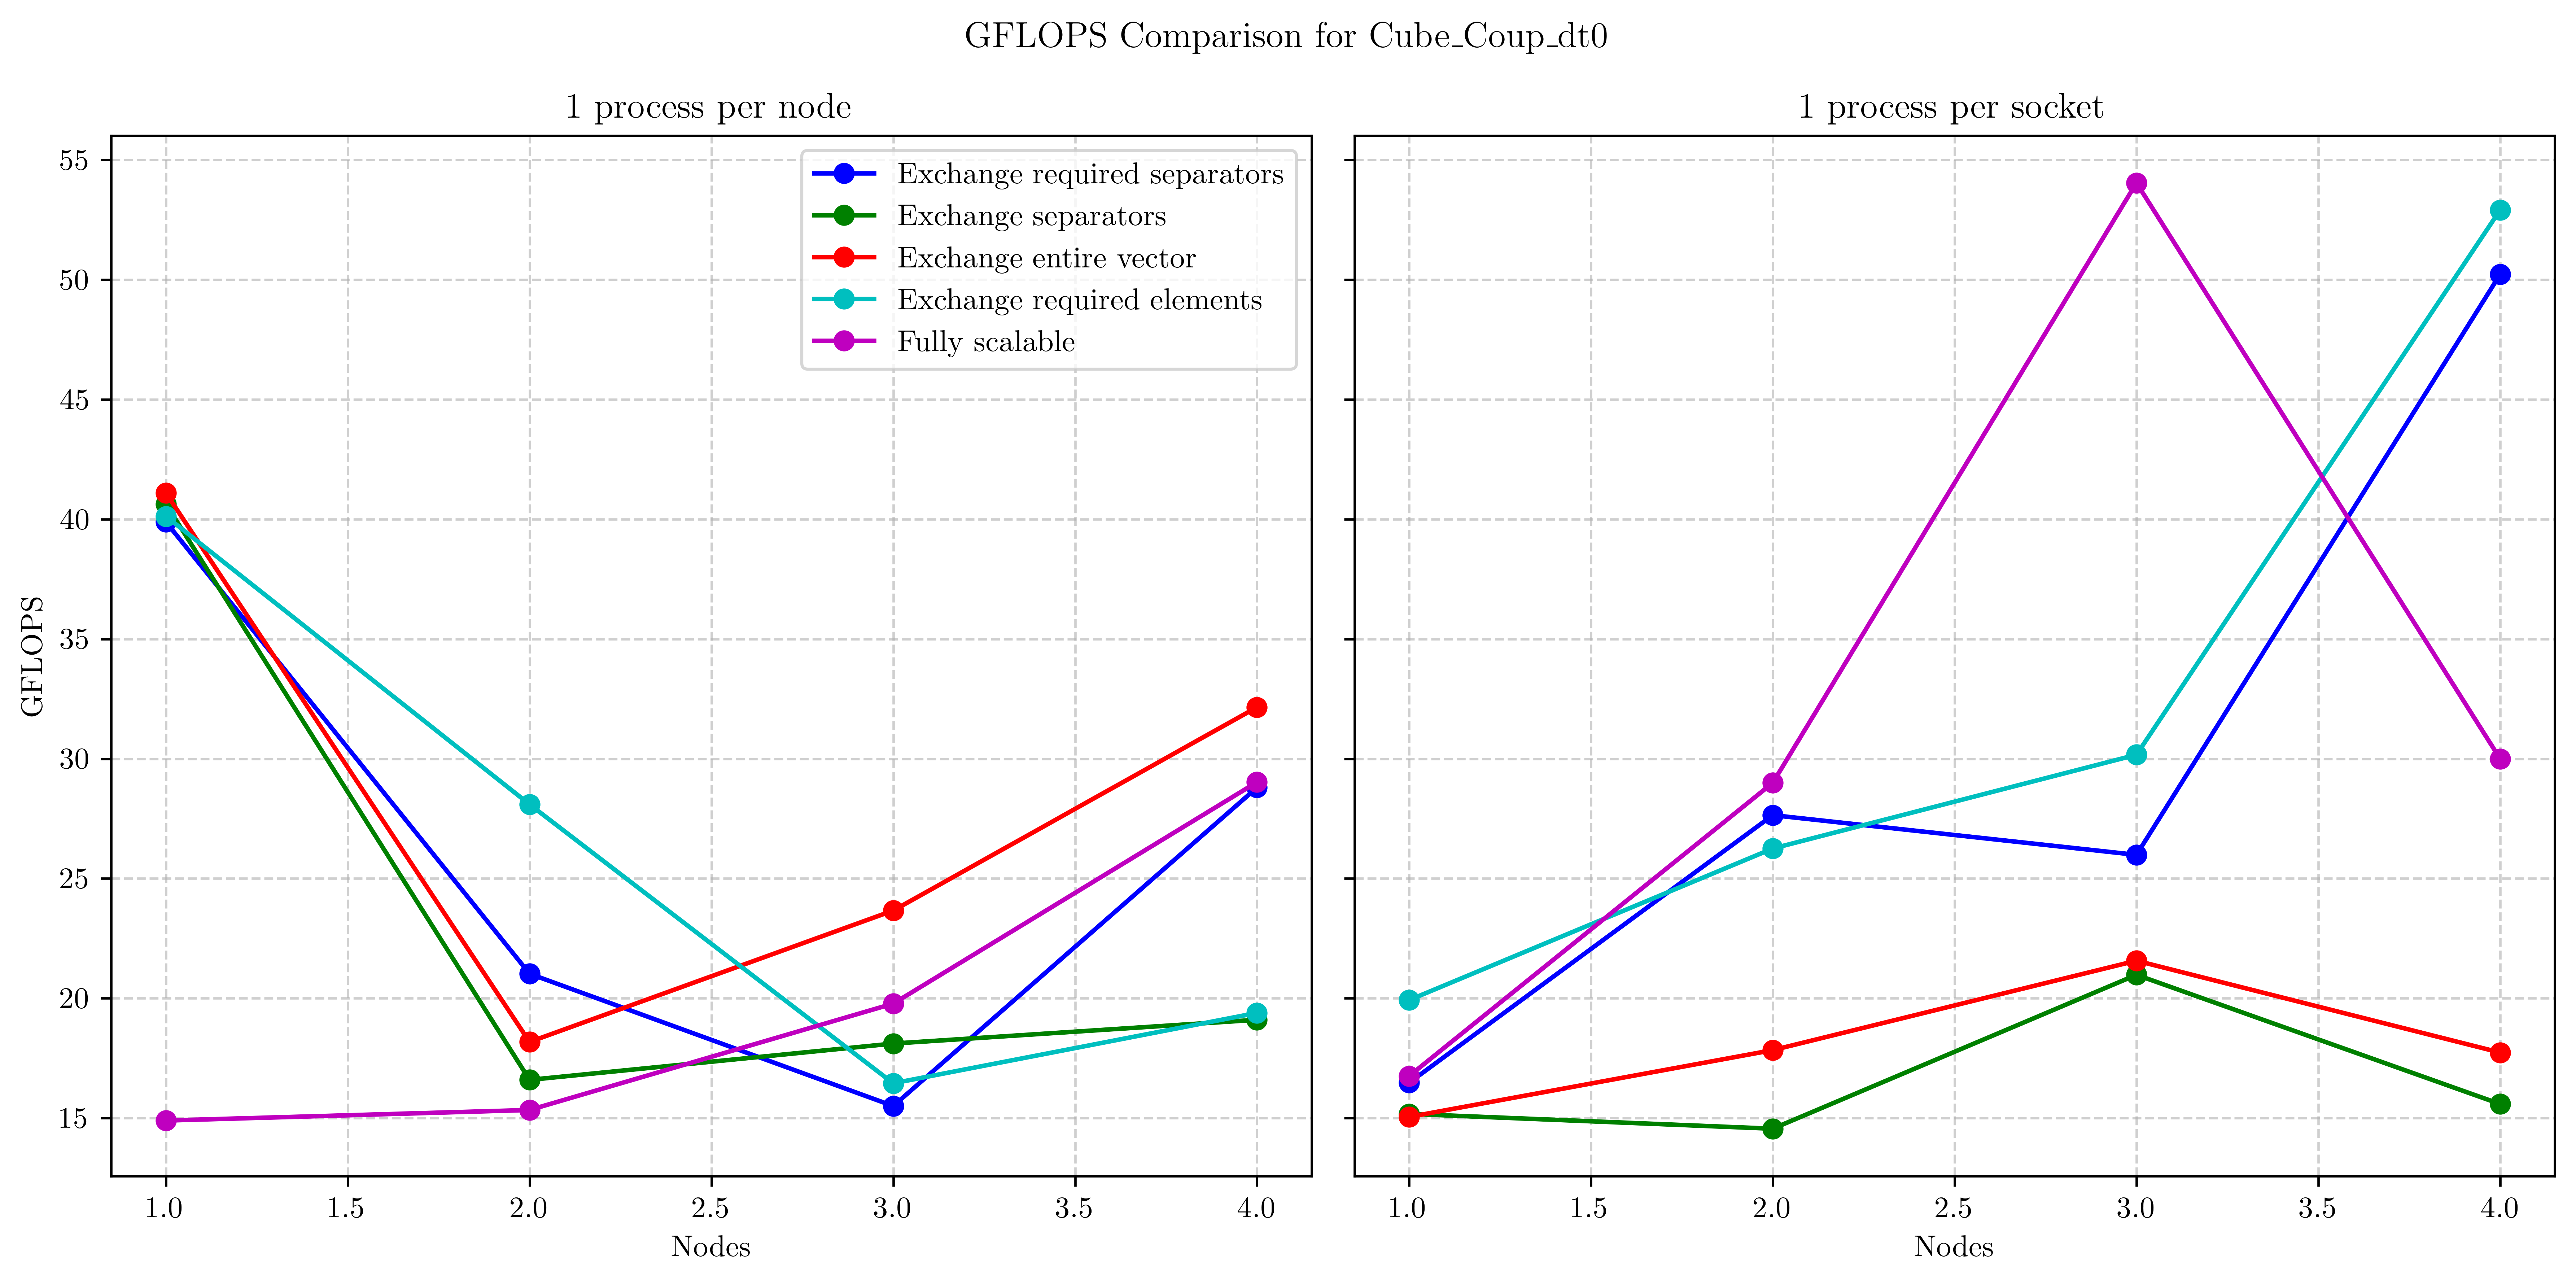
\includegraphics[width=0.95\textwidth]{Cube_Coup_dt0_fpgaq}
    \end{center}
    \caption{Cube\_Coup\_dt0}
    \label{fig:Cube_Coup_dt0_fpgaq}
\end{figure}

\begin{figure}[H]
    \begin{center}
        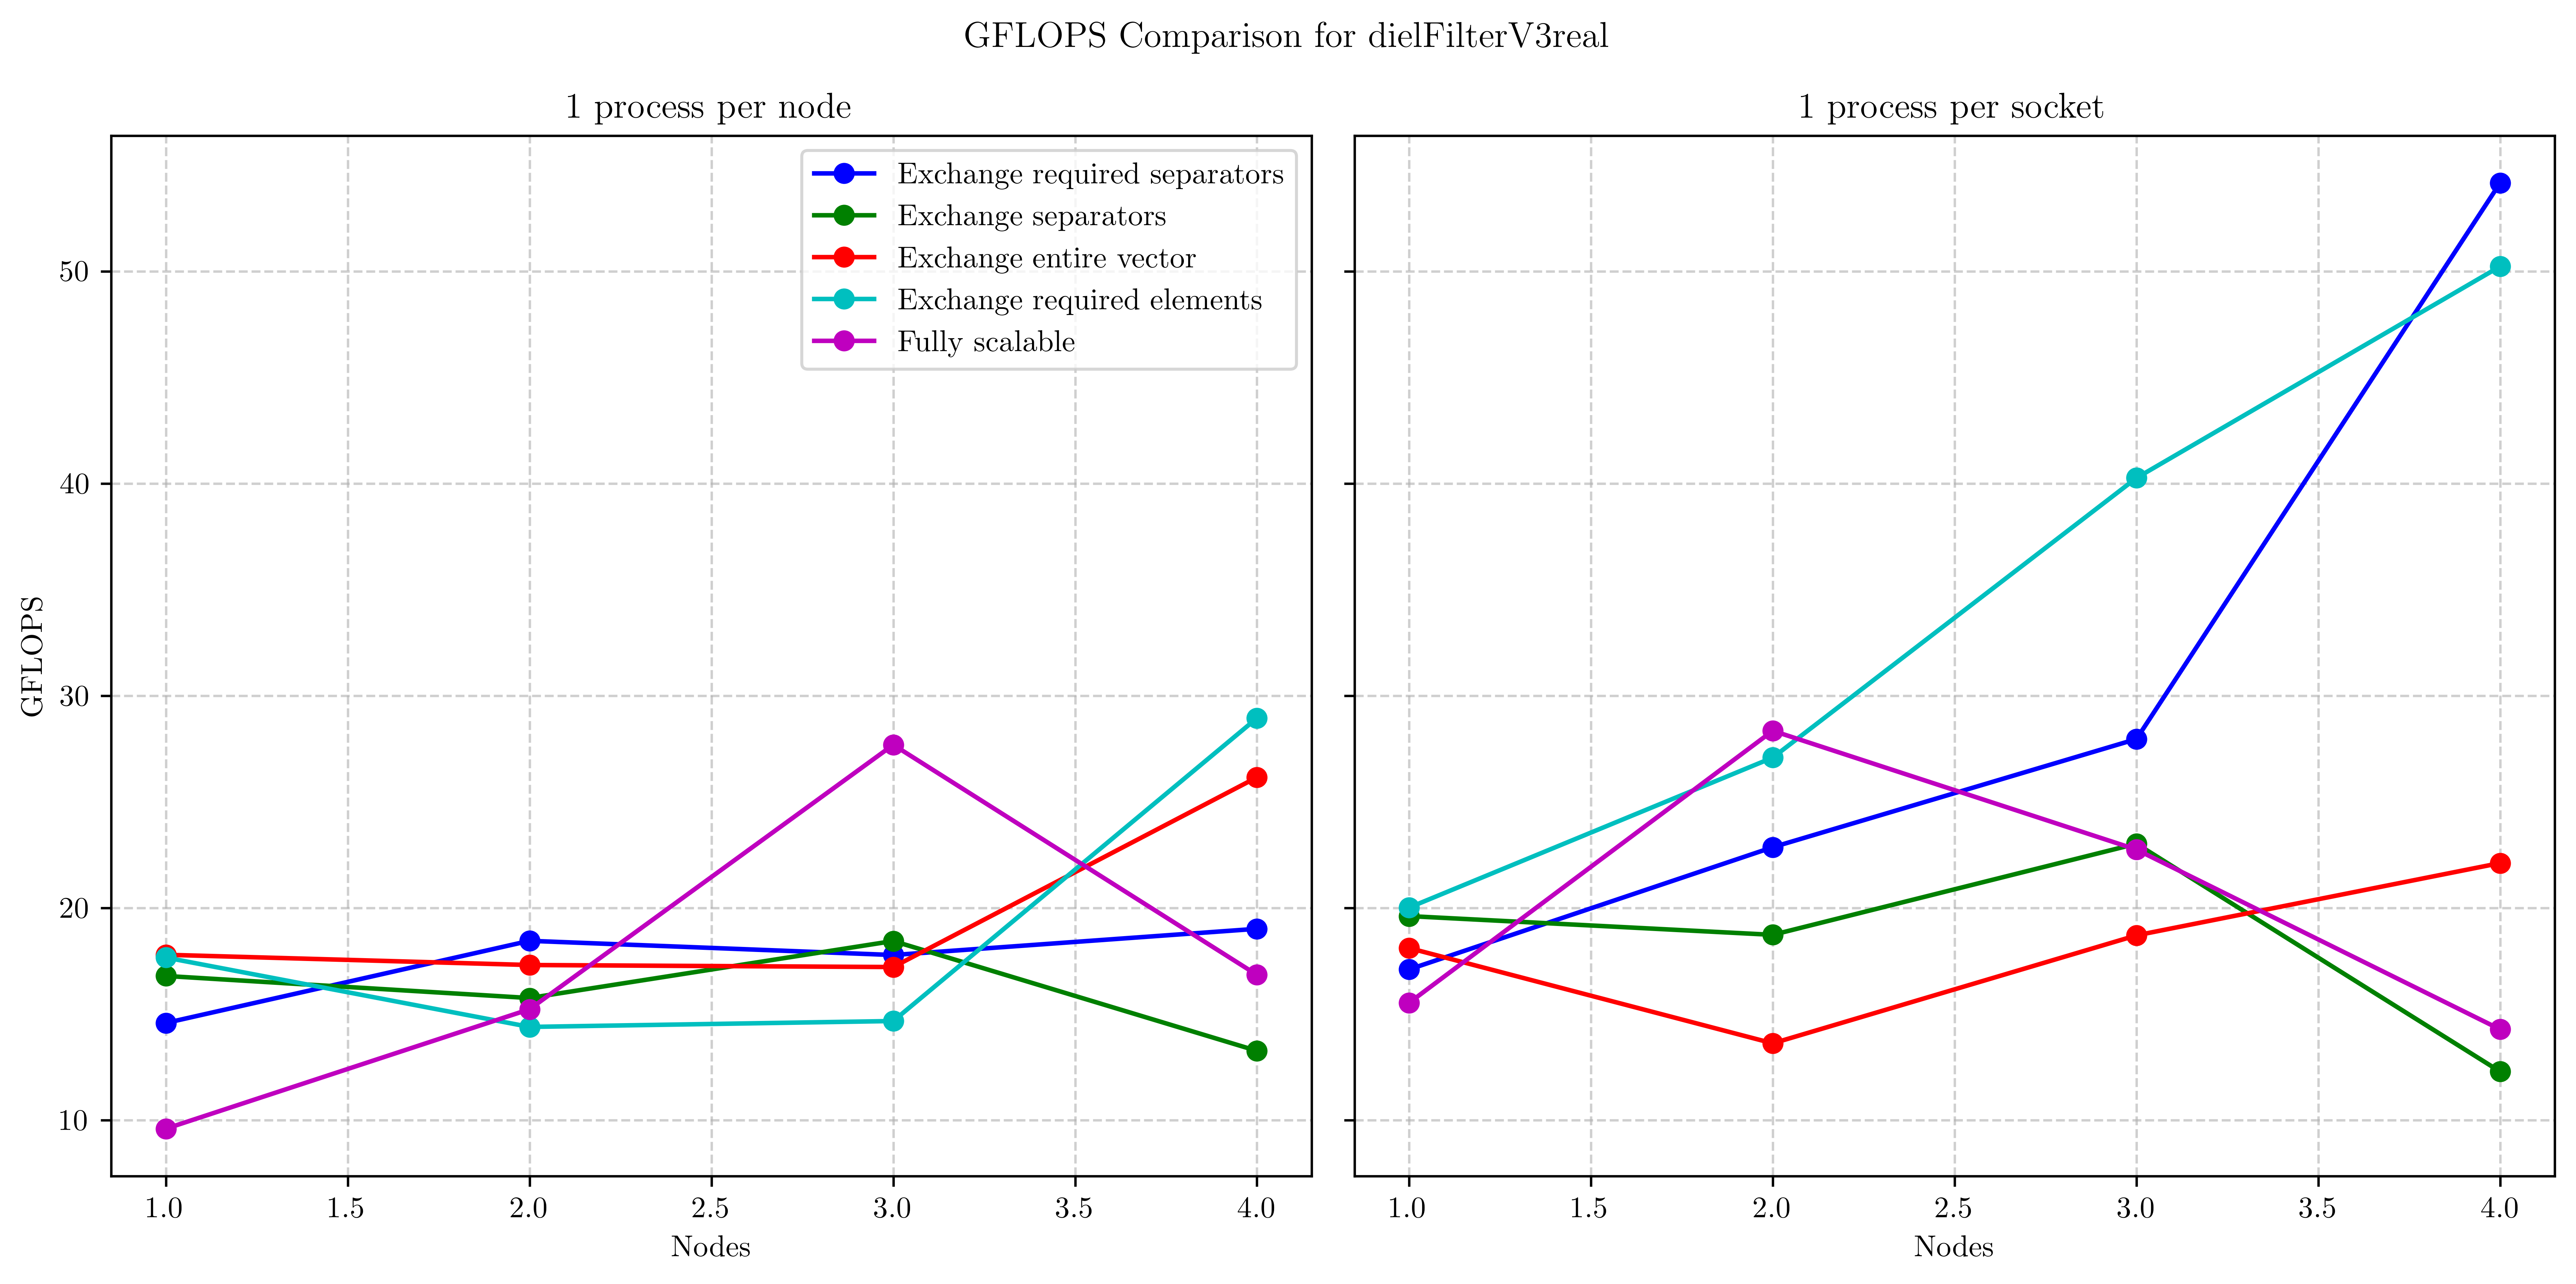
\includegraphics[width=0.95\textwidth]{dielFilterV3real_fpgaq}
    \end{center}
    \caption{dielFilterV3real}
    \label{fig:dielFilterV3real_fpgaq}
\end{figure}


\begin{figure}[H]
    \begin{center}
        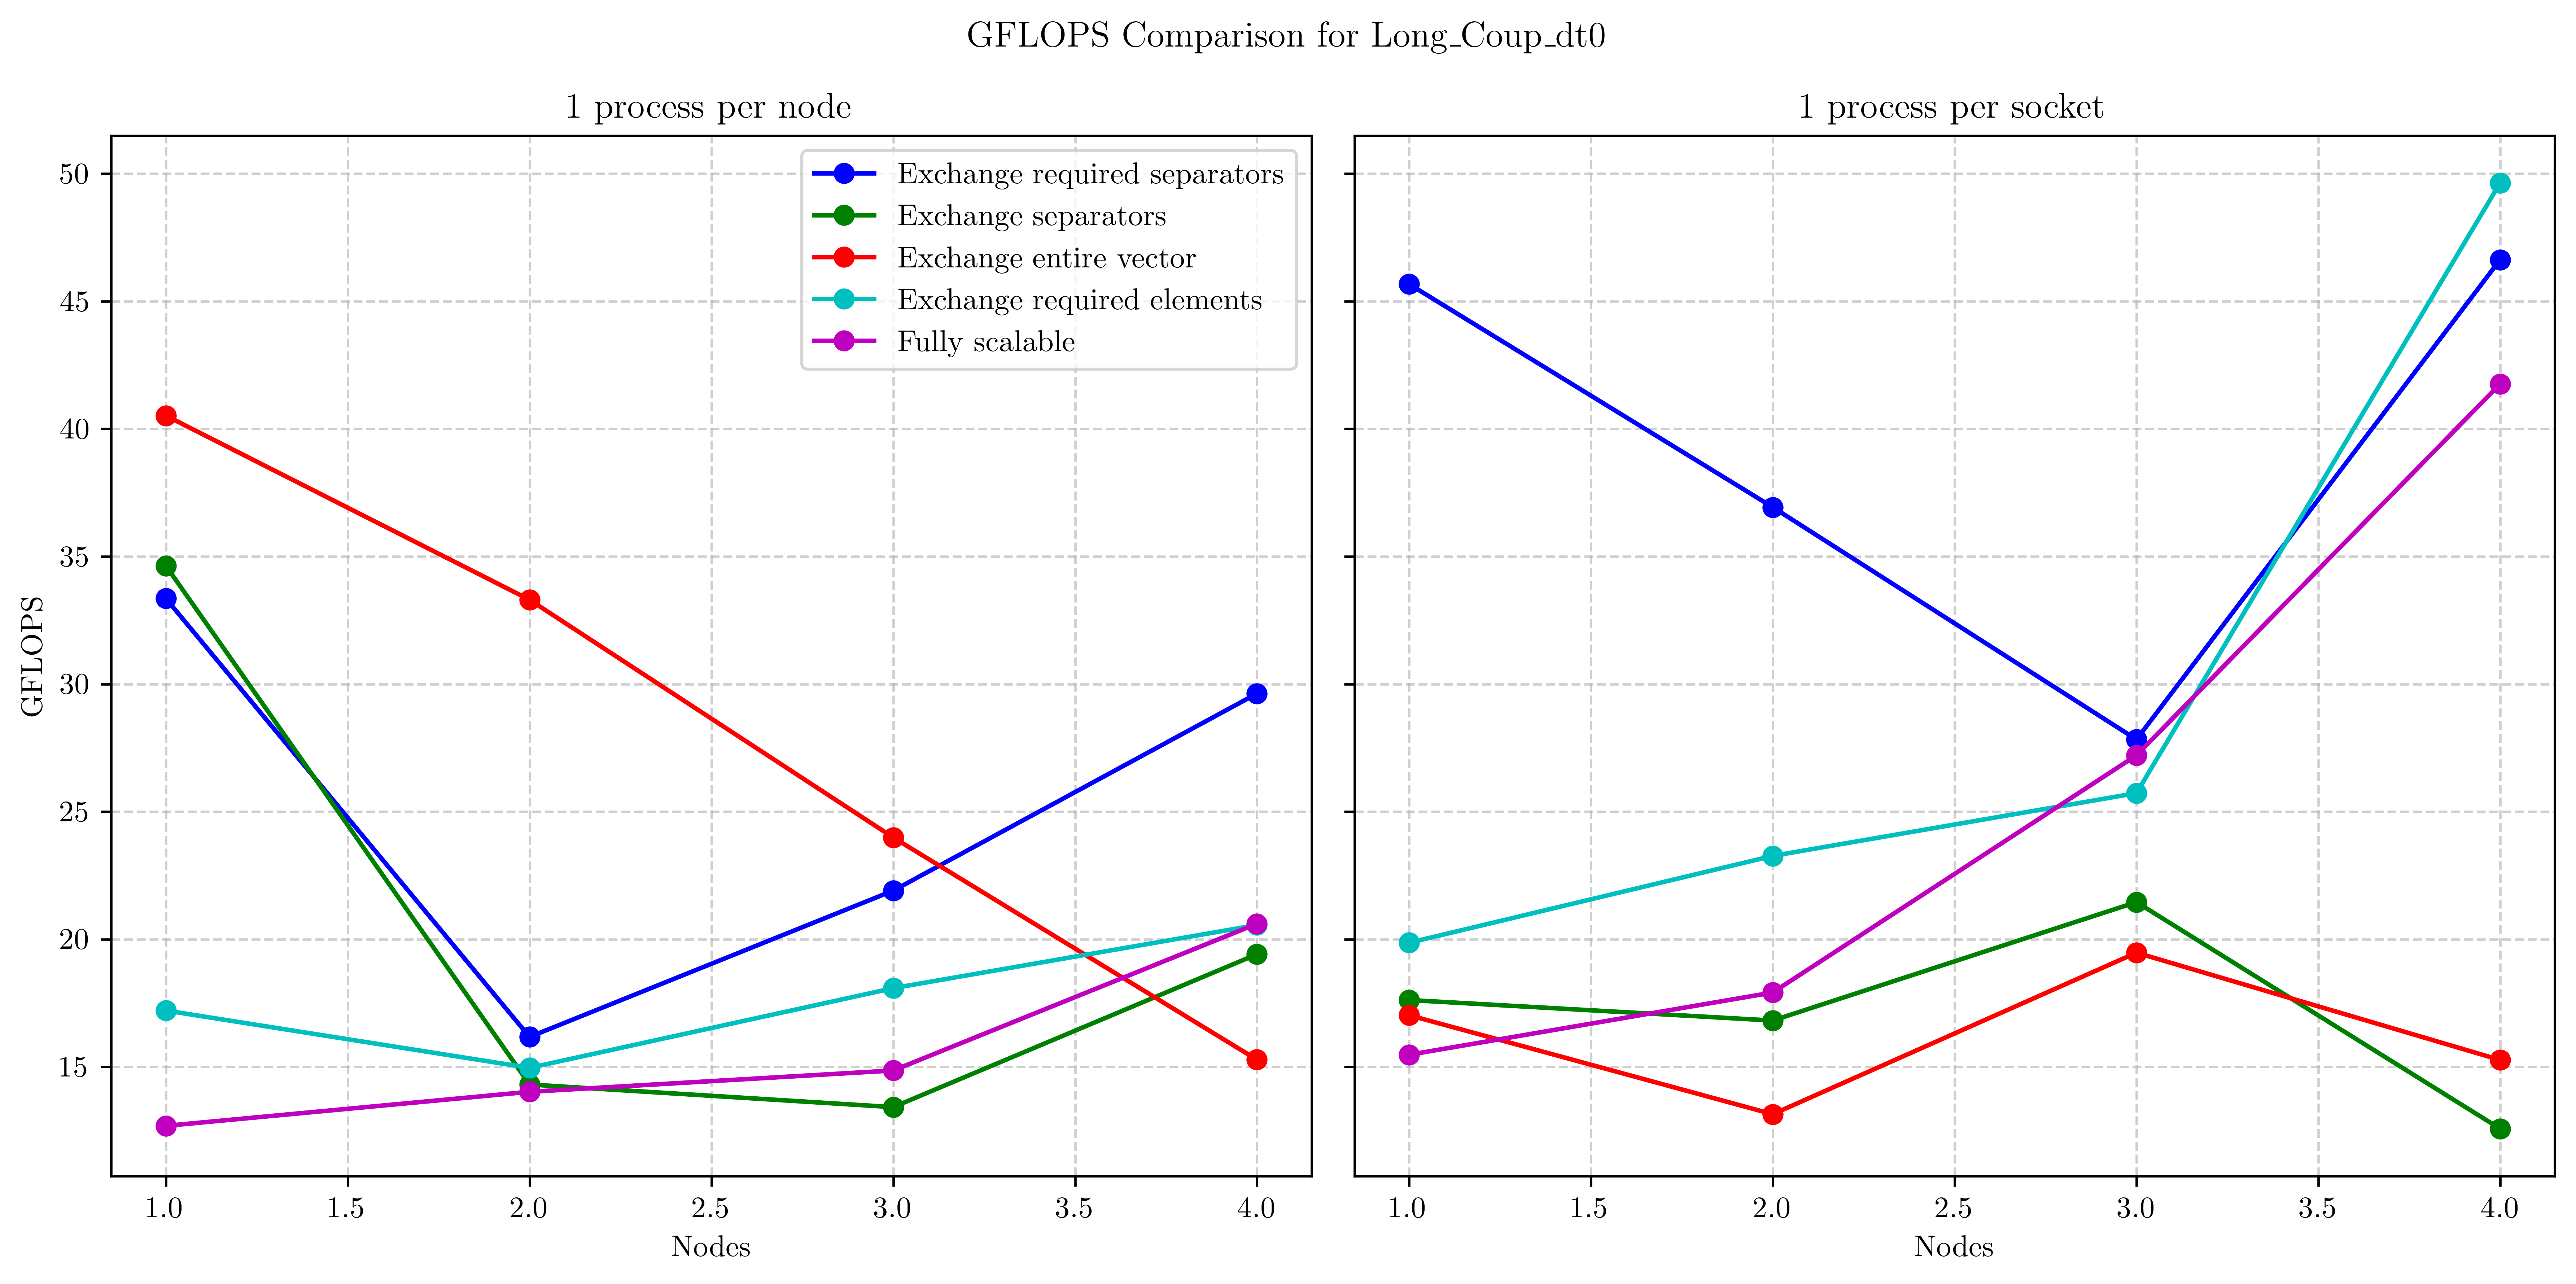
\includegraphics[width=0.95\textwidth]{Long_Coup_dt0_fpgaq}
    \end{center}
    \caption{Long\_Coup\_dt0}
    \label{fig:Long_Coup_dt0_fpgaq}
\end{figure}

\begin{figure}[H]
    \begin{center}
        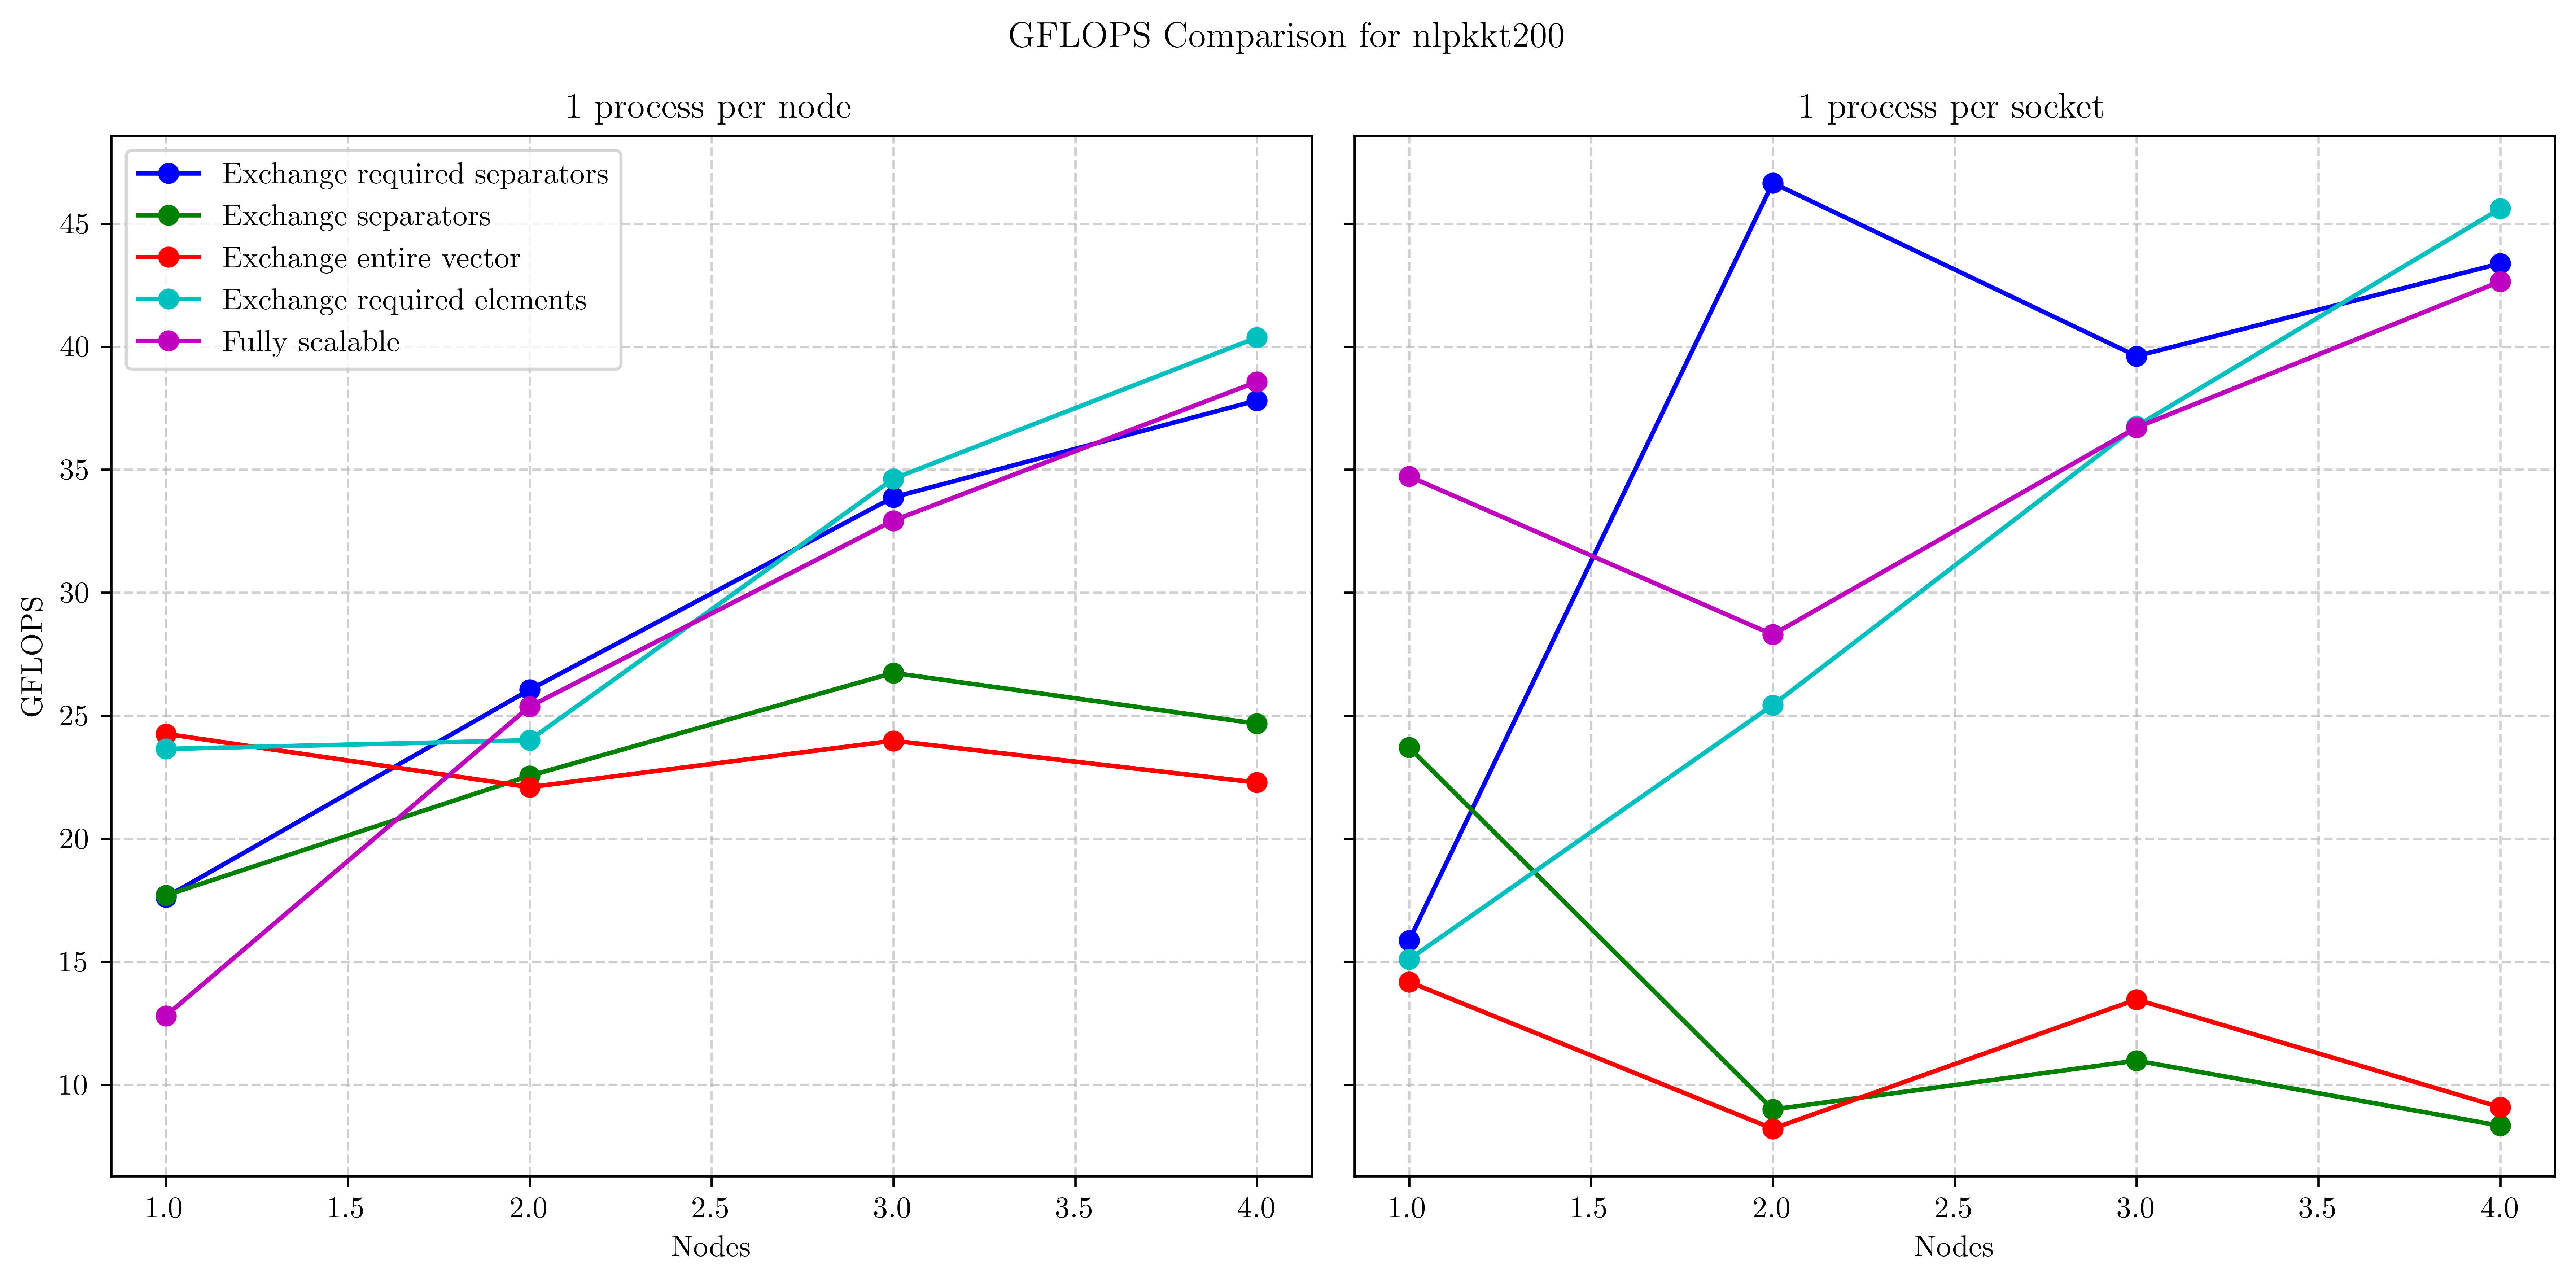
\includegraphics[width=0.95\textwidth]{nlpkkt200_fpgaq}
    \end{center}
    \caption{nlpkkt200}
    \label{fig:nlpkkt200_fpgaq}
\end{figure}


% \begin{figure}[H]
%     \begin{center}
%         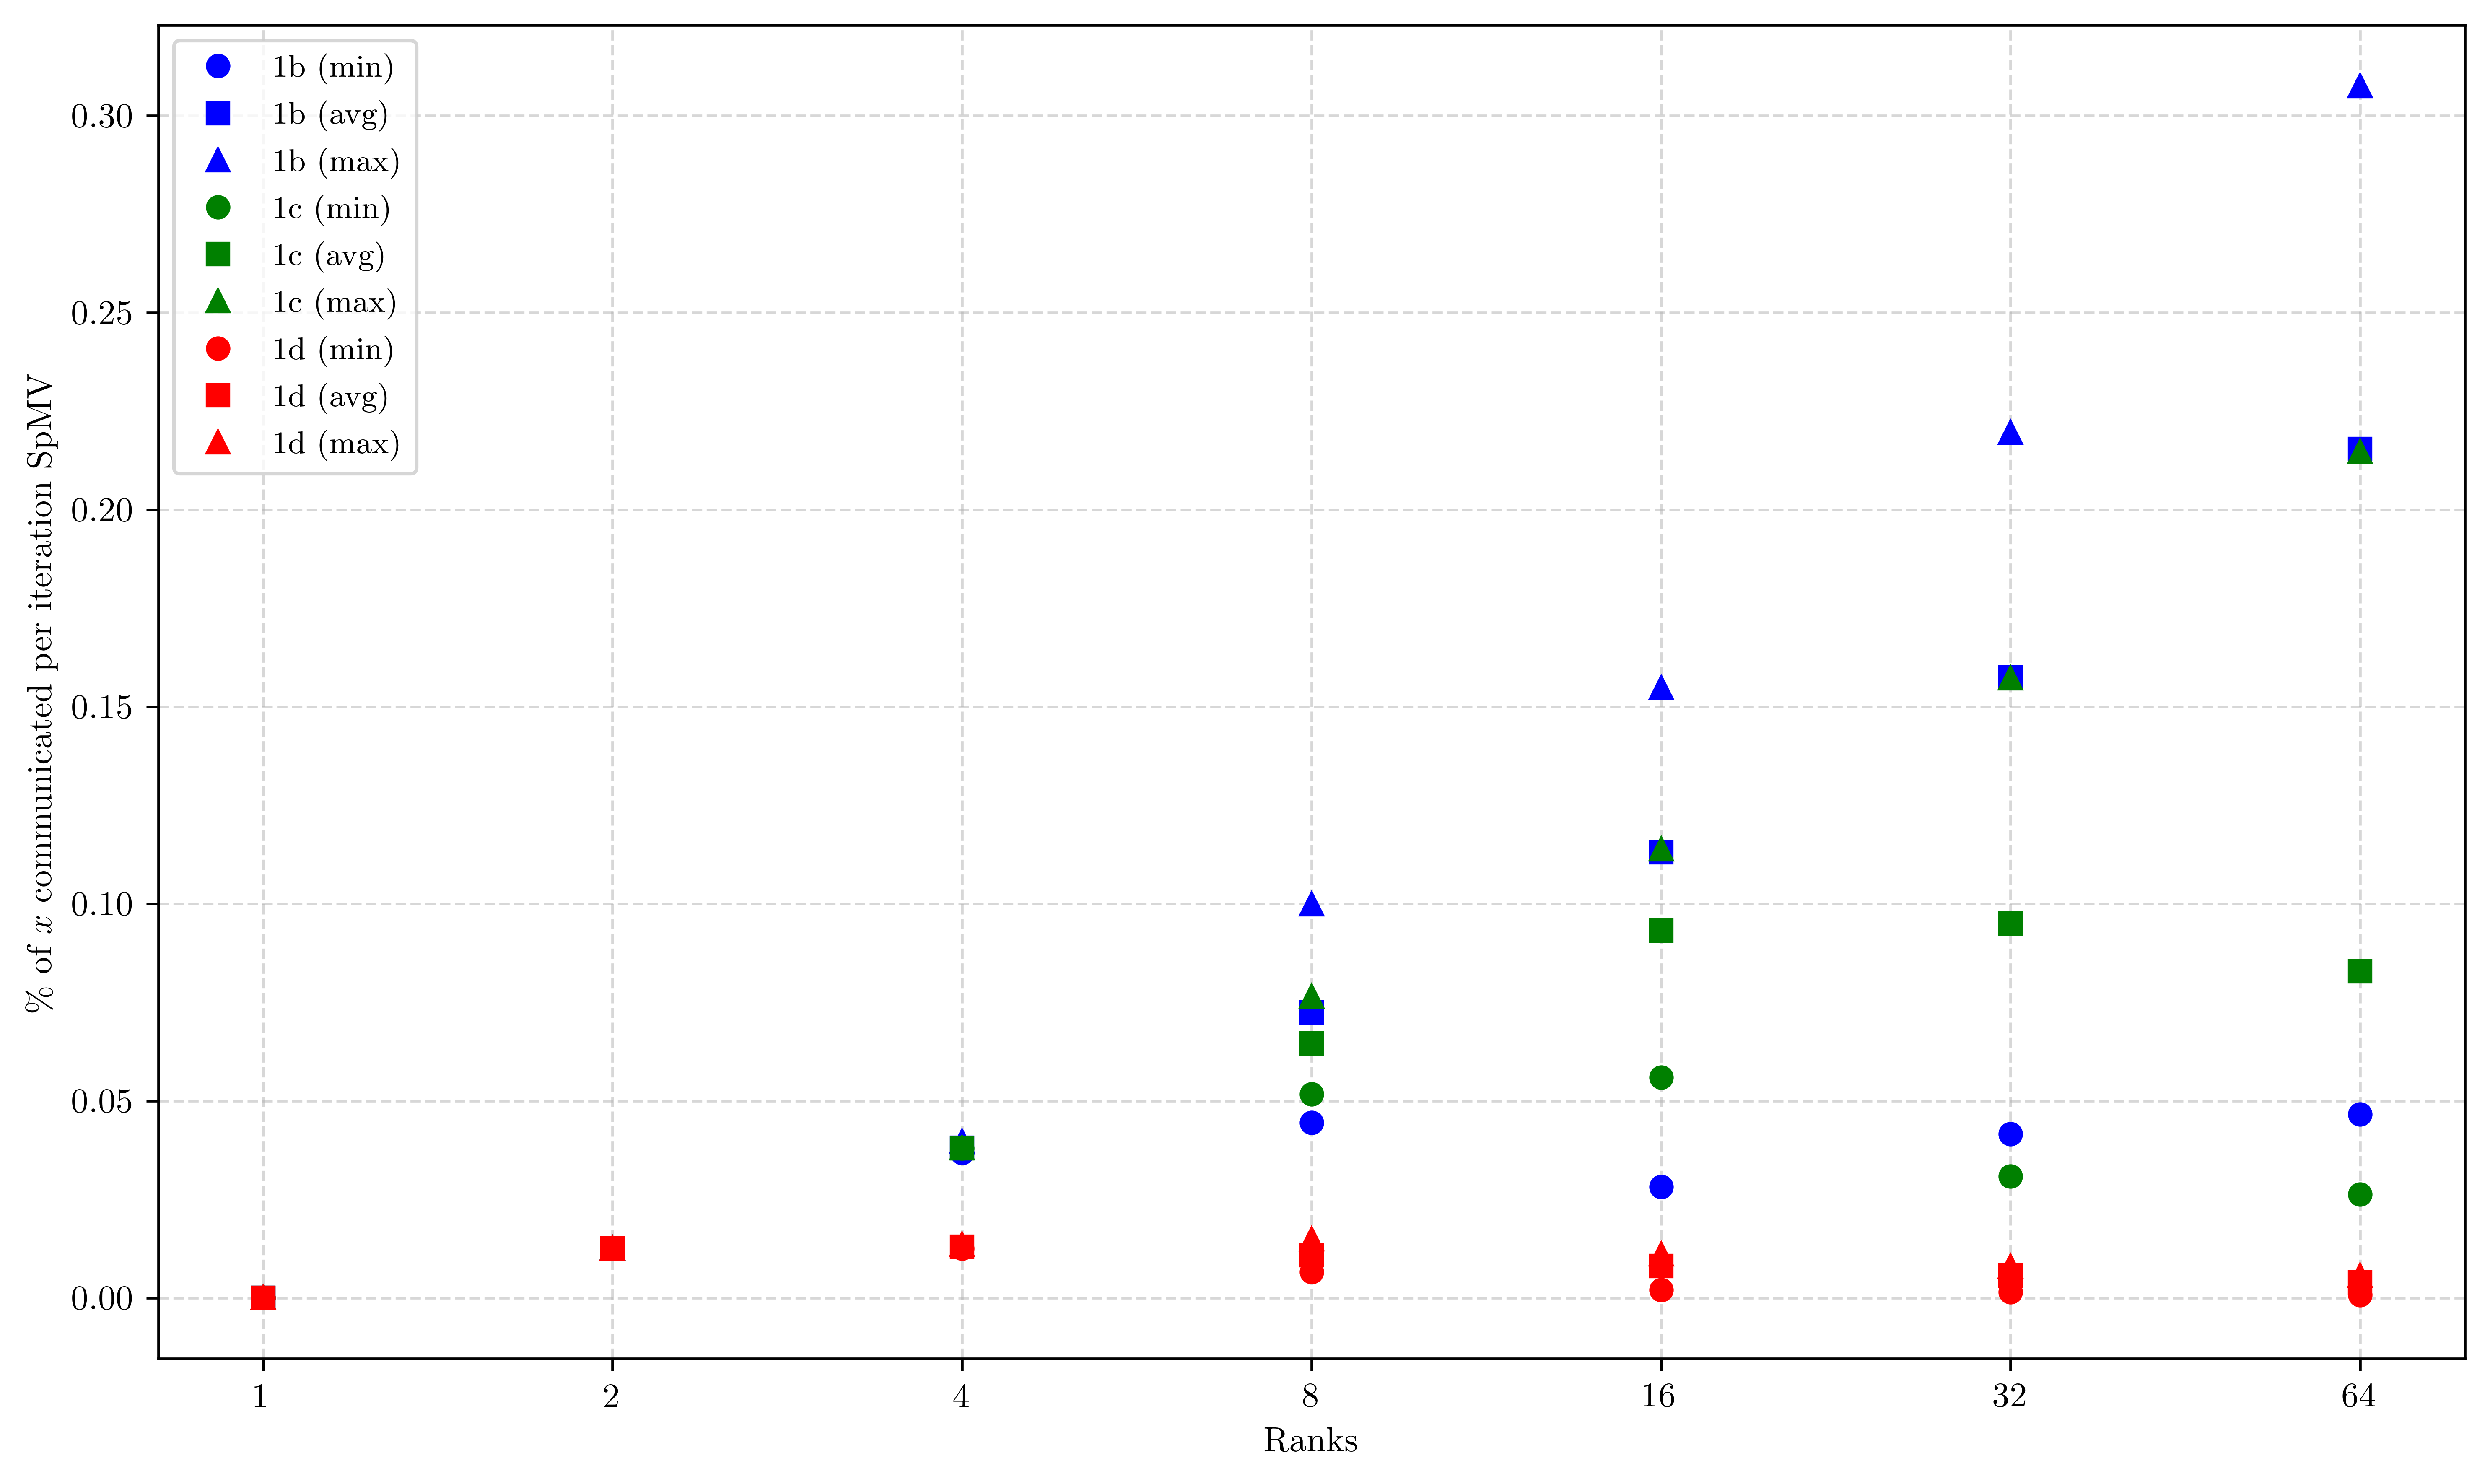
\includegraphics[width=0.95\textwidth]{Serena_defq_commload_single.png}
%     \end{center}
%     \title{Communication load serena \defq}
%     \caption{}
%     \label{fig:Serena_defq_commload_single.png}
% \end{figure}

% \begin{figure}[H]
%     \begin{center}
%         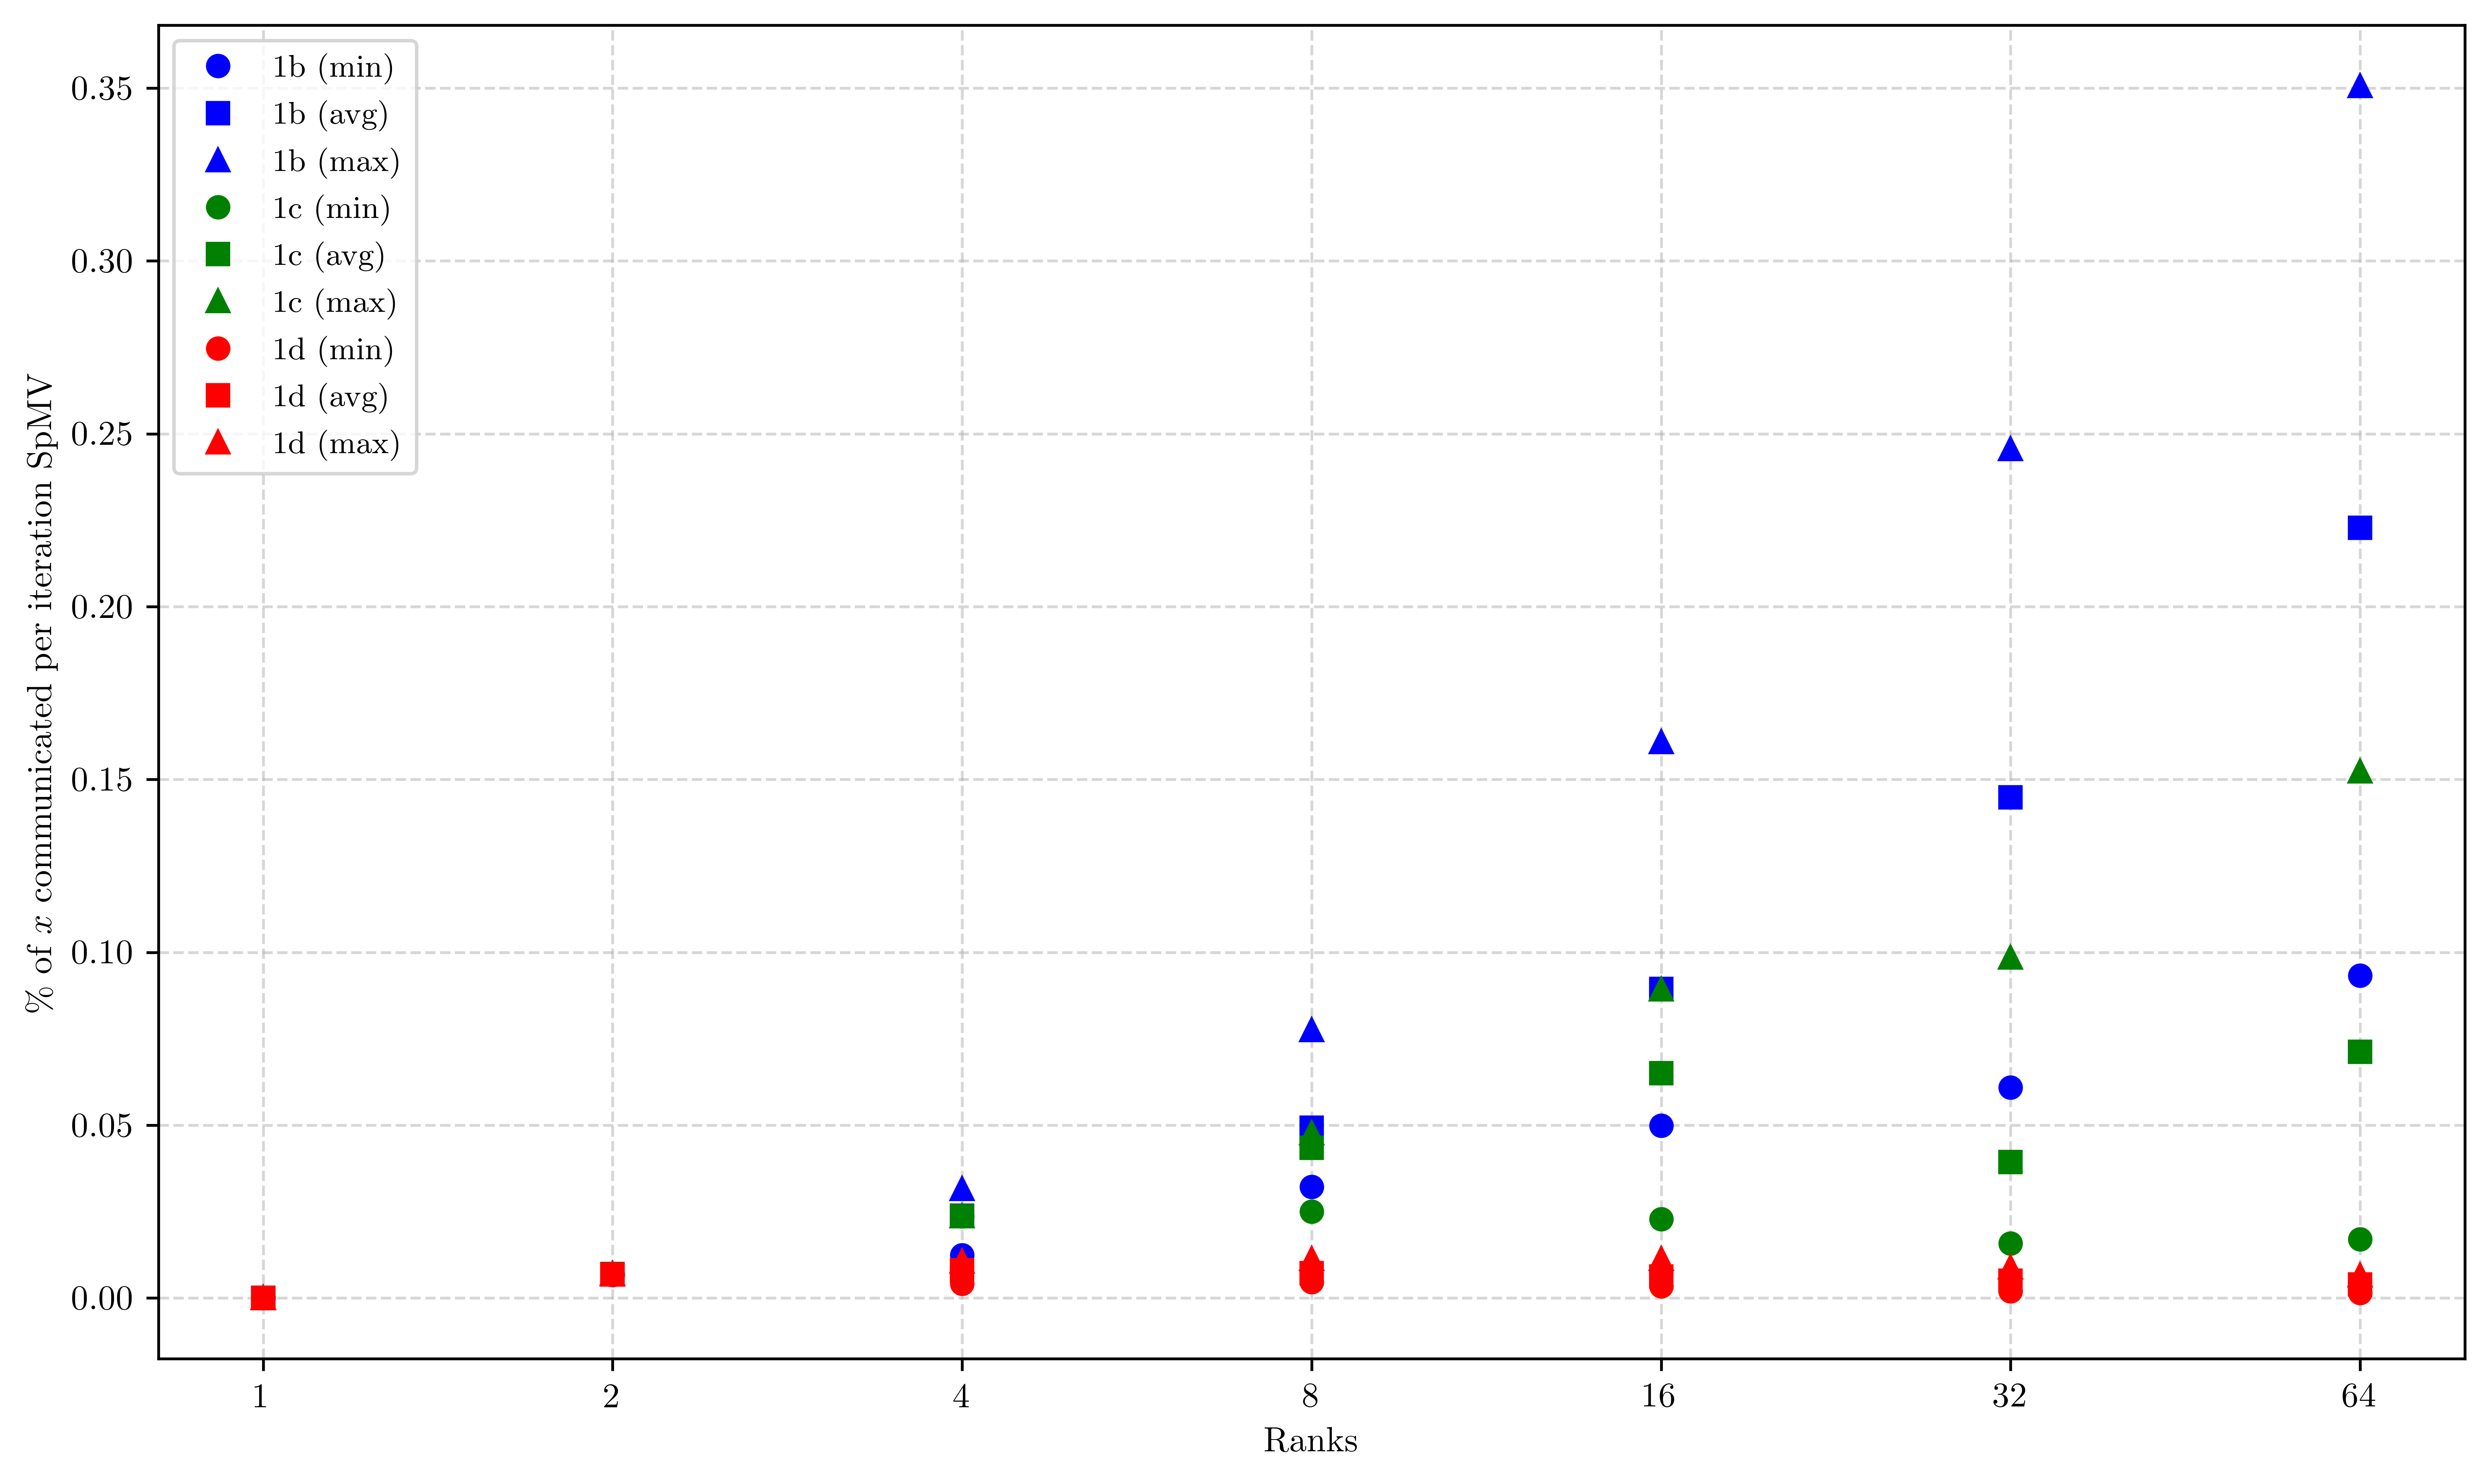
\includegraphics[width=0.95\textwidth]{bone010_defq_commload_single.png}
%     \end{center}
%     \caption{}
%     \label{fig:bone010_defq_commload_single.png}
% \end{figure}

% \begin{figure}[H]
%     \begin{center}
%         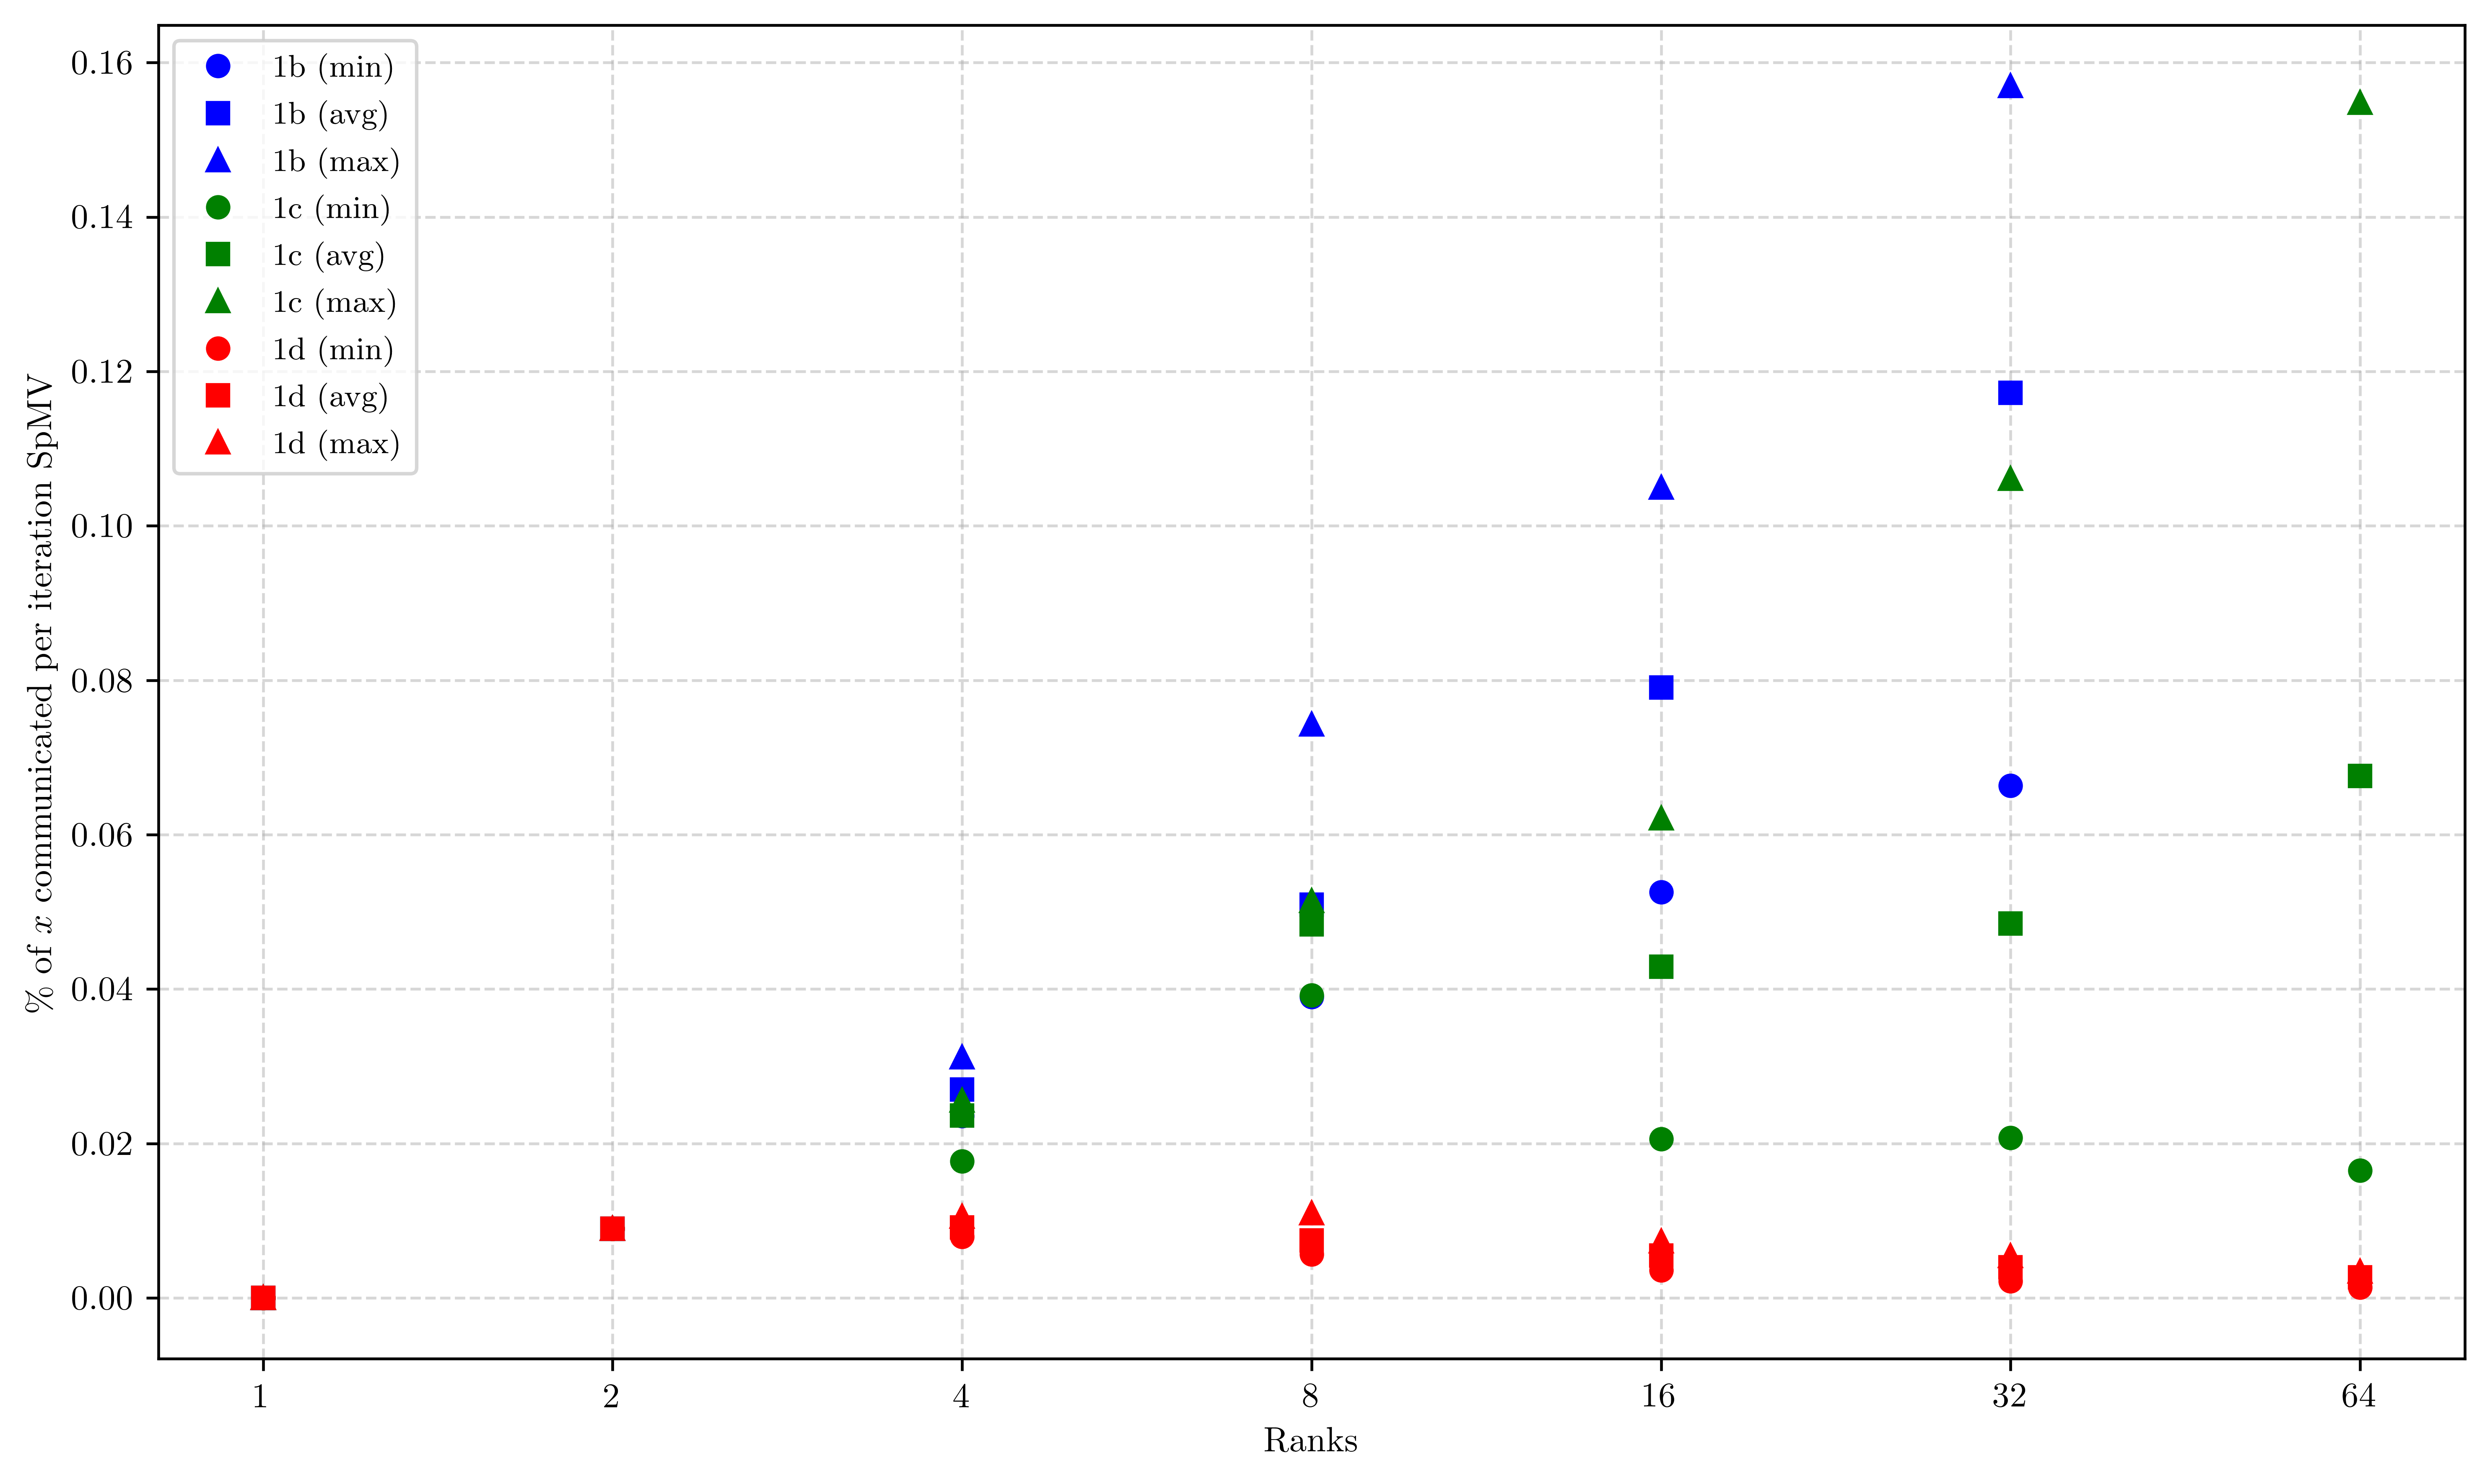
\includegraphics[width=0.95\textwidth]{nlpkkt200_defq_commload_single.png}
%     \end{center}
%     \caption{}
%     \label{fig:nlpkkt200_defq_commload_single.png}
% \end{figure}


\subsection{Communication time}

\begin{figure}[H]
    \begin{center}
        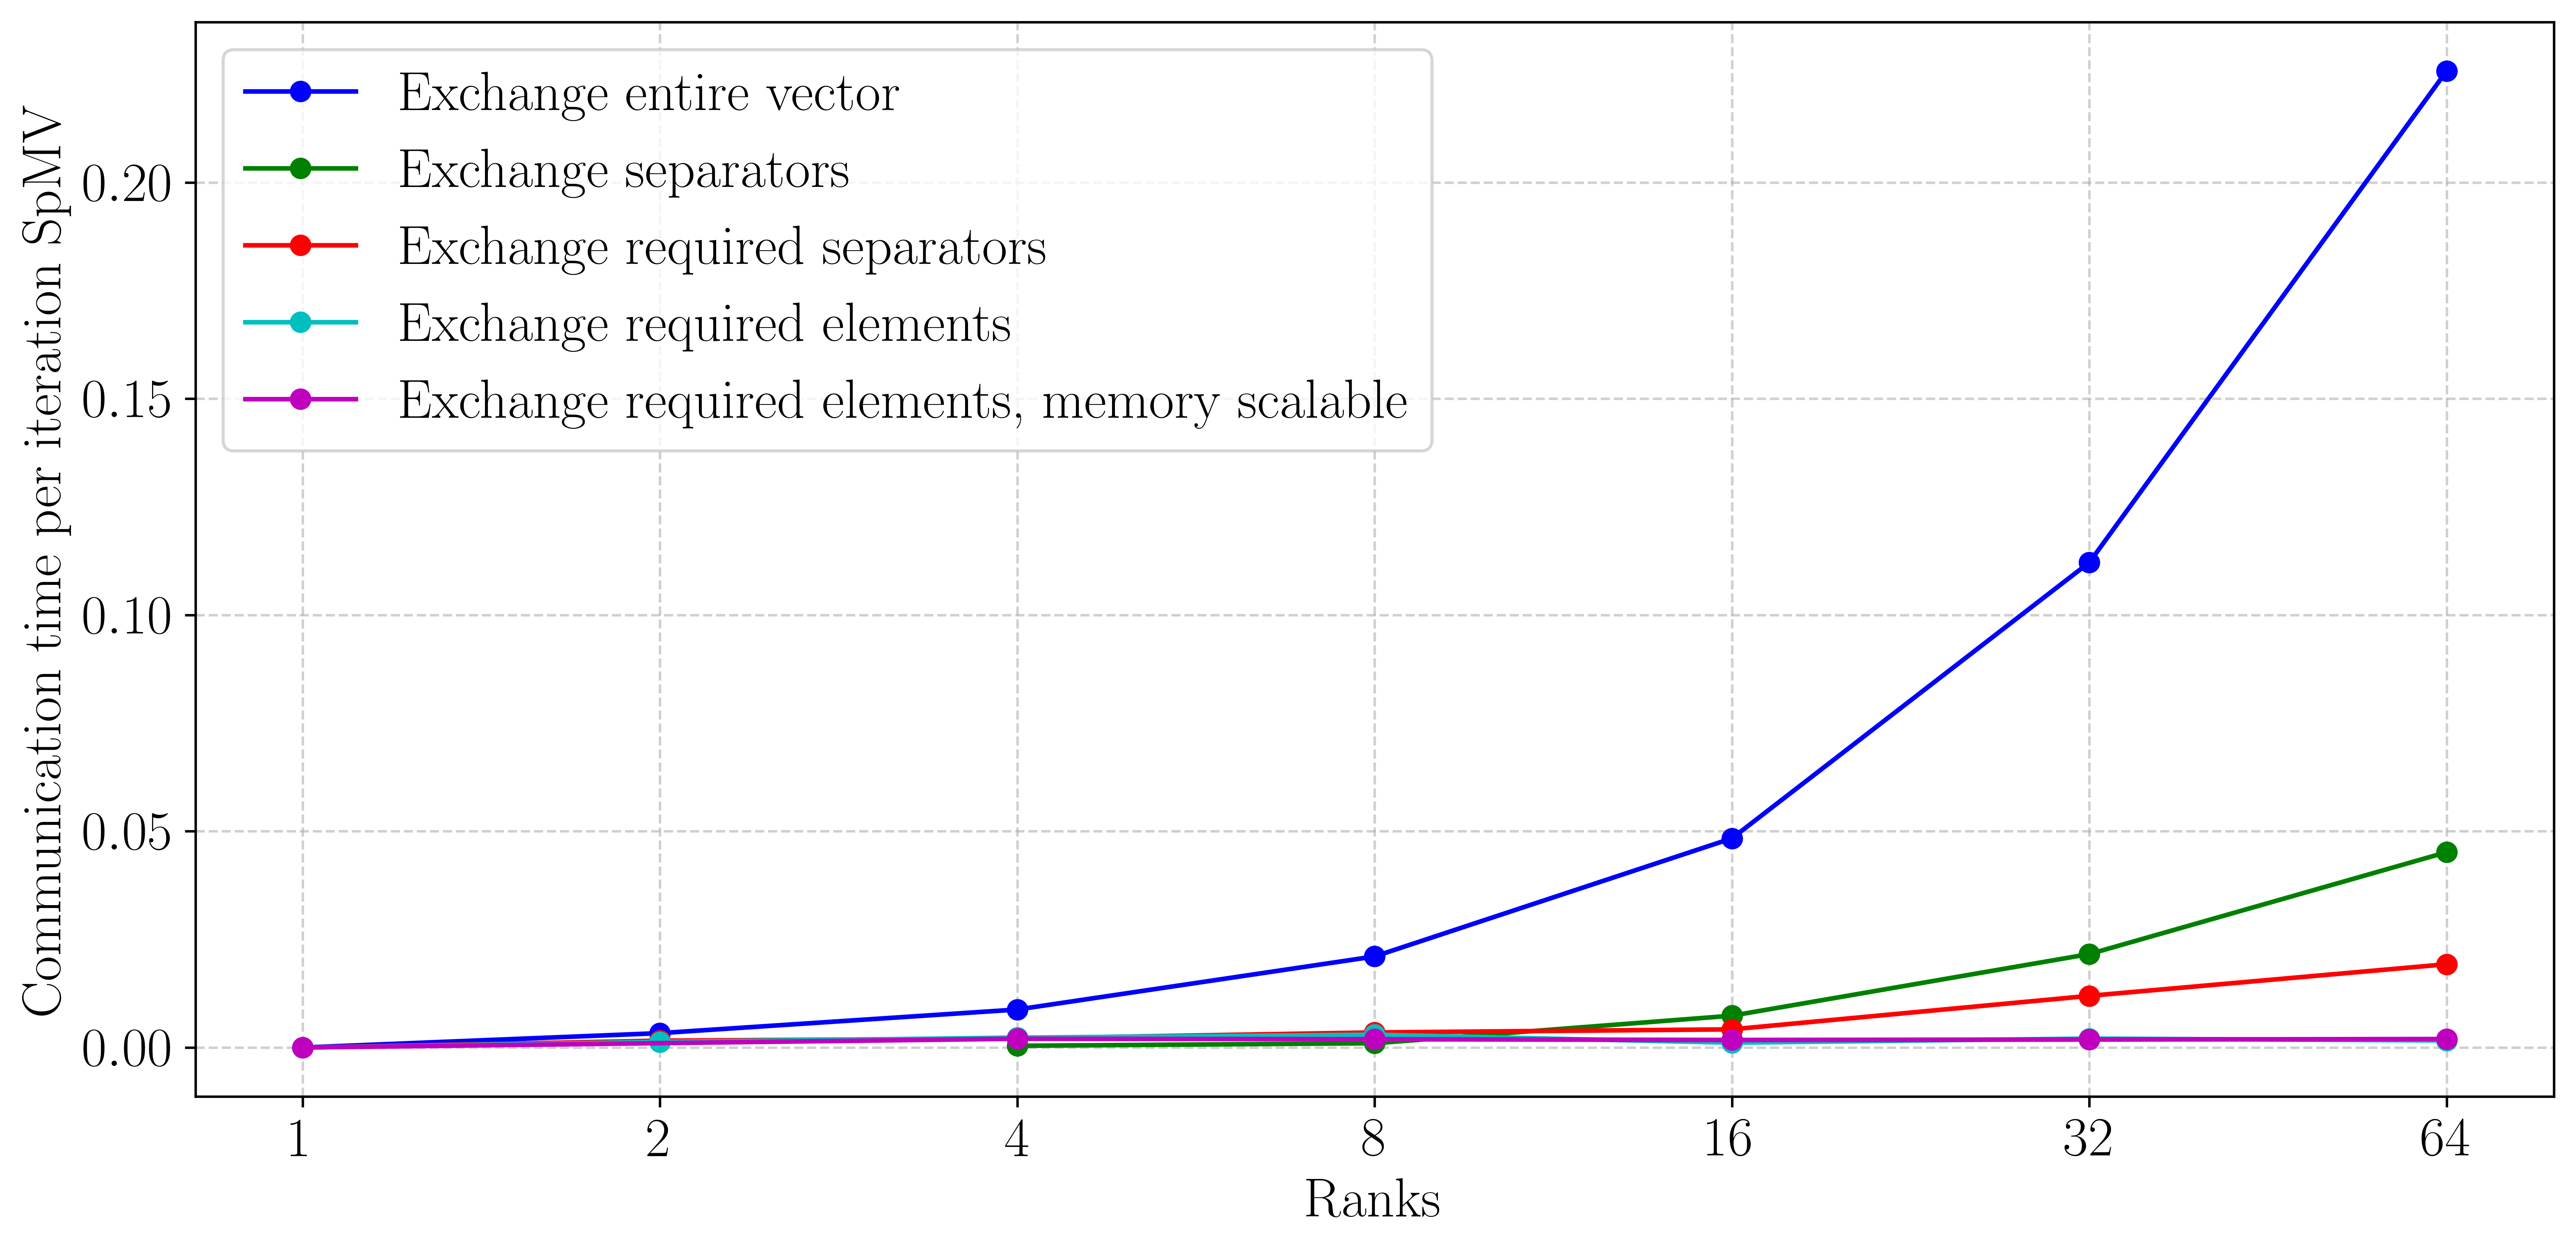
\includegraphics[width=0.95\textwidth]{Serena_tcomm_single_defq.png}
    \end{center}
    \caption{}
    \label{fig:Serena_tcomm_single_defq.png}
\end{figure}


\begin{figure}[H]
    \begin{center}
        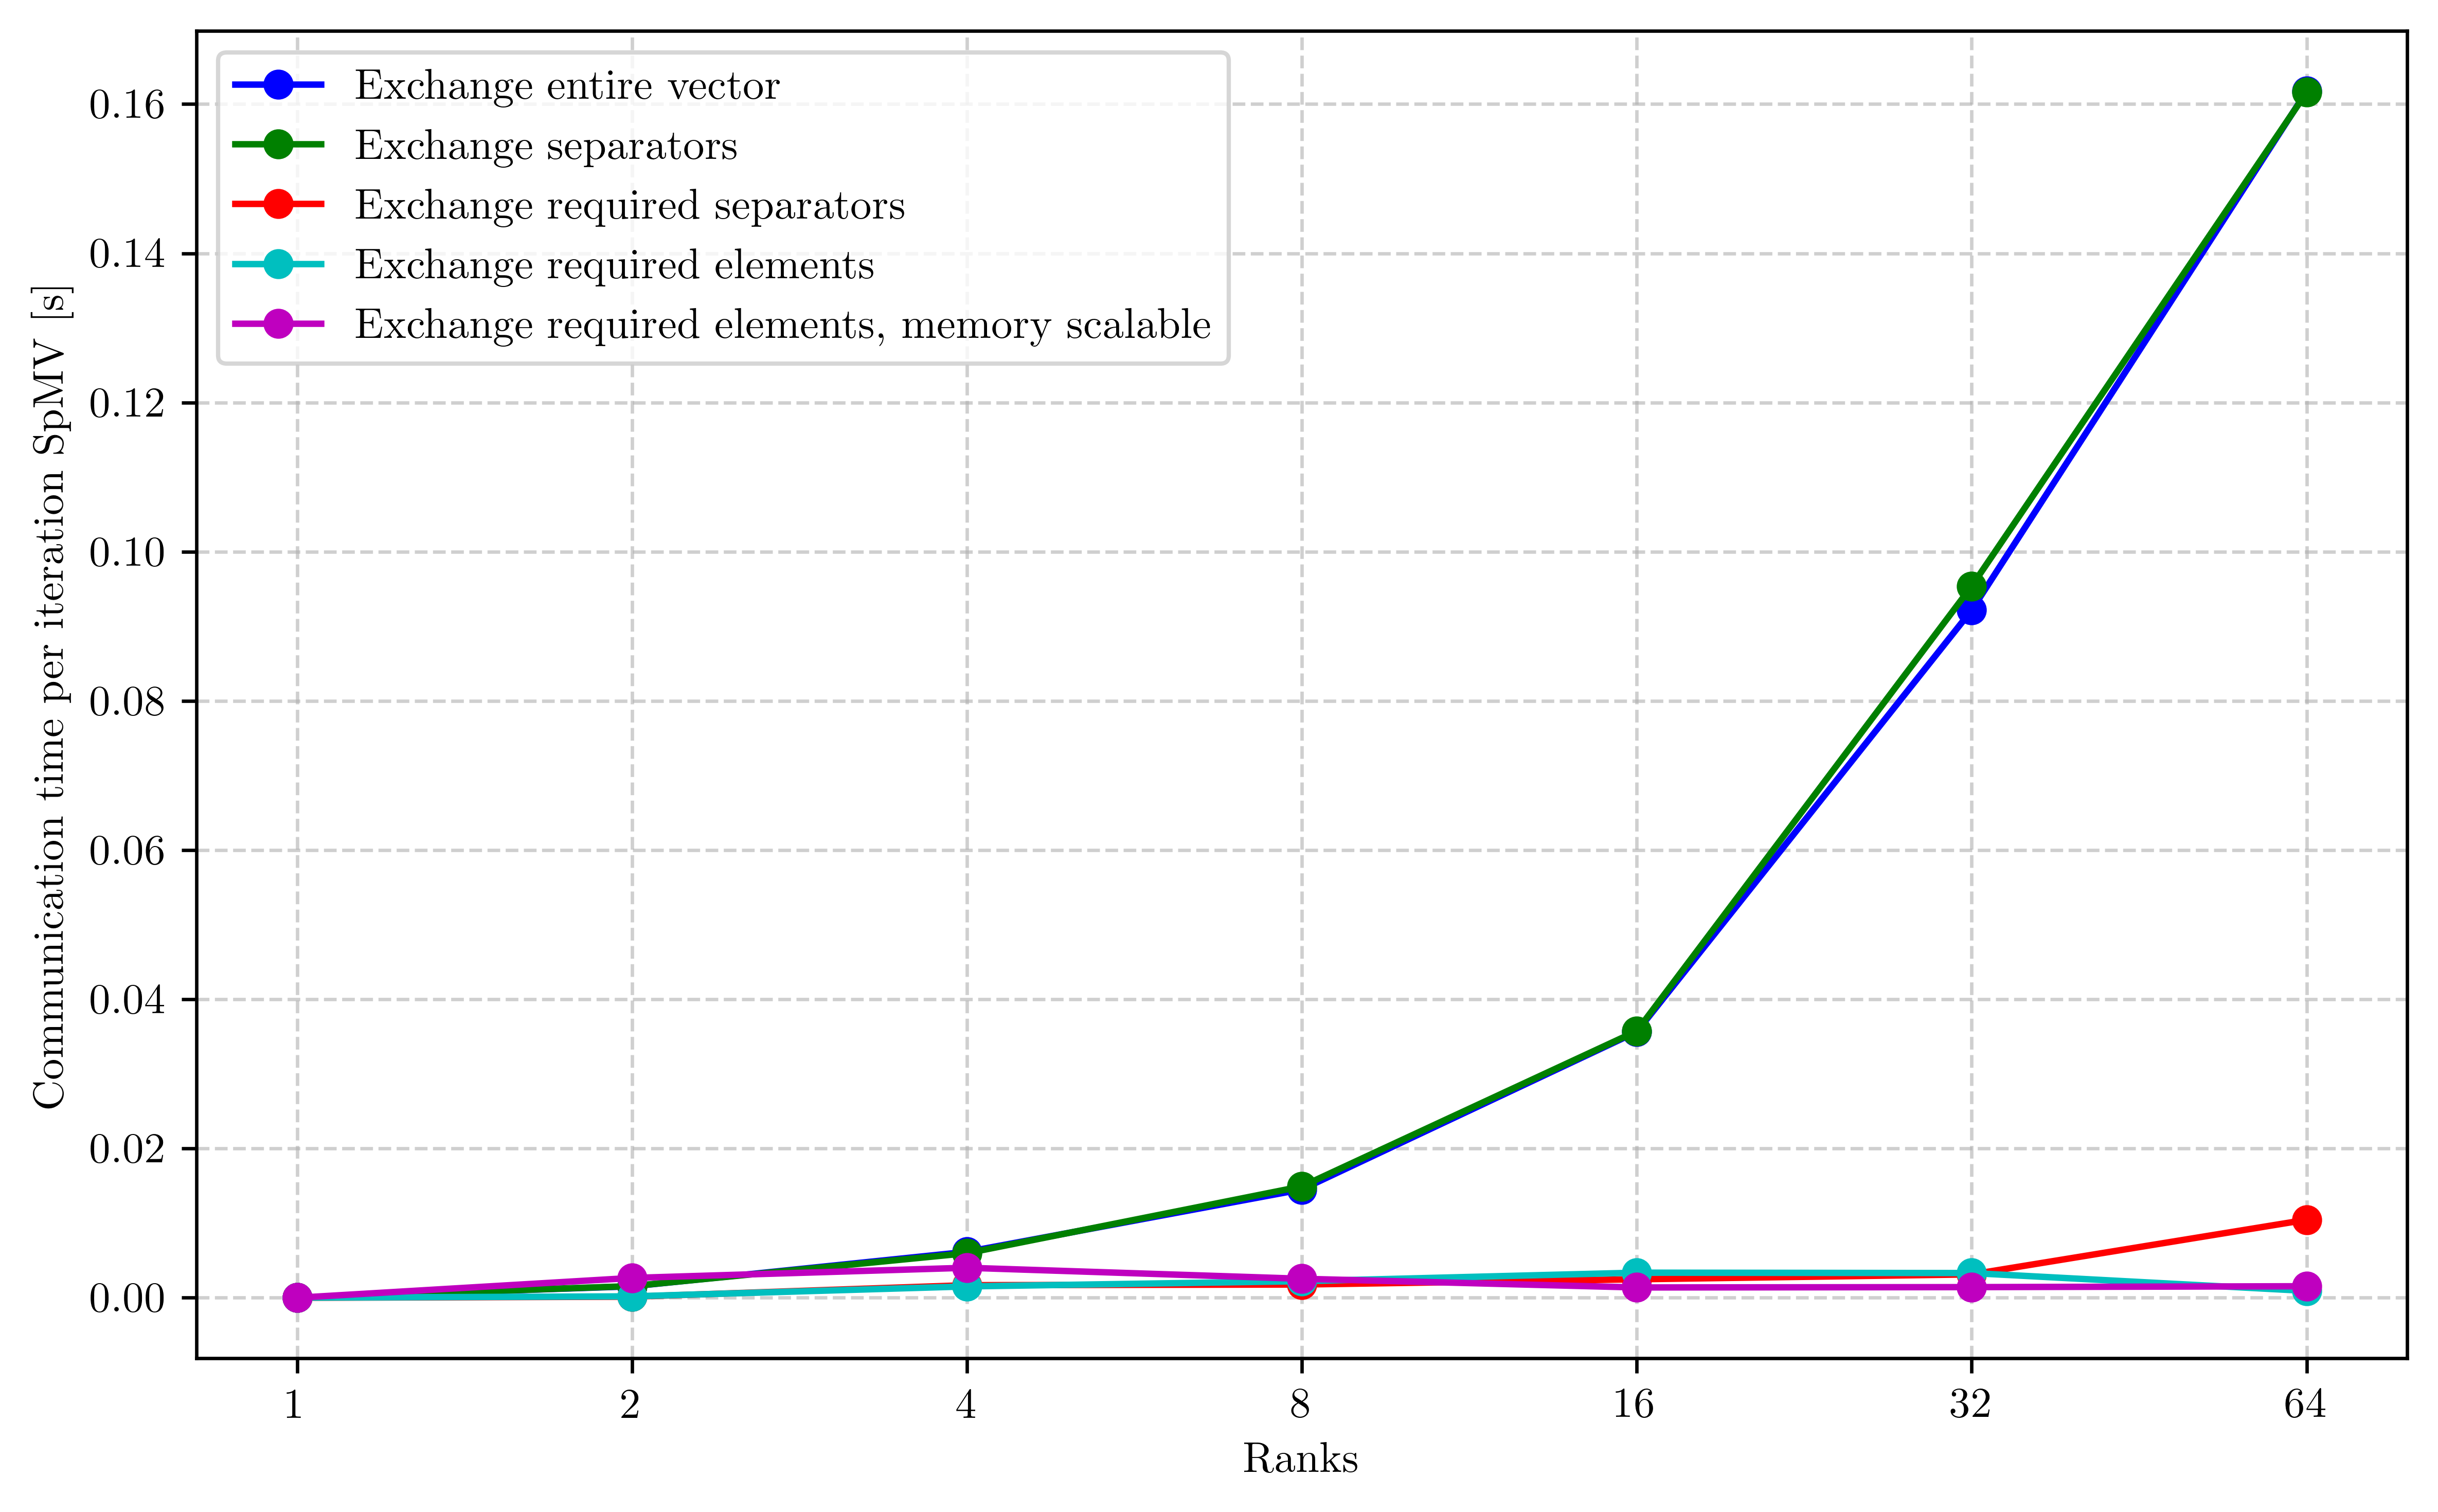
\includegraphics[width=0.95\textwidth]{bone010_tcomm_single_defq.png}
    \end{center}
    \caption{}
    \label{fig:bone010_tcomm_single_defq.png}
\end{figure}

\begin{figure}[H]
    \begin{center}
        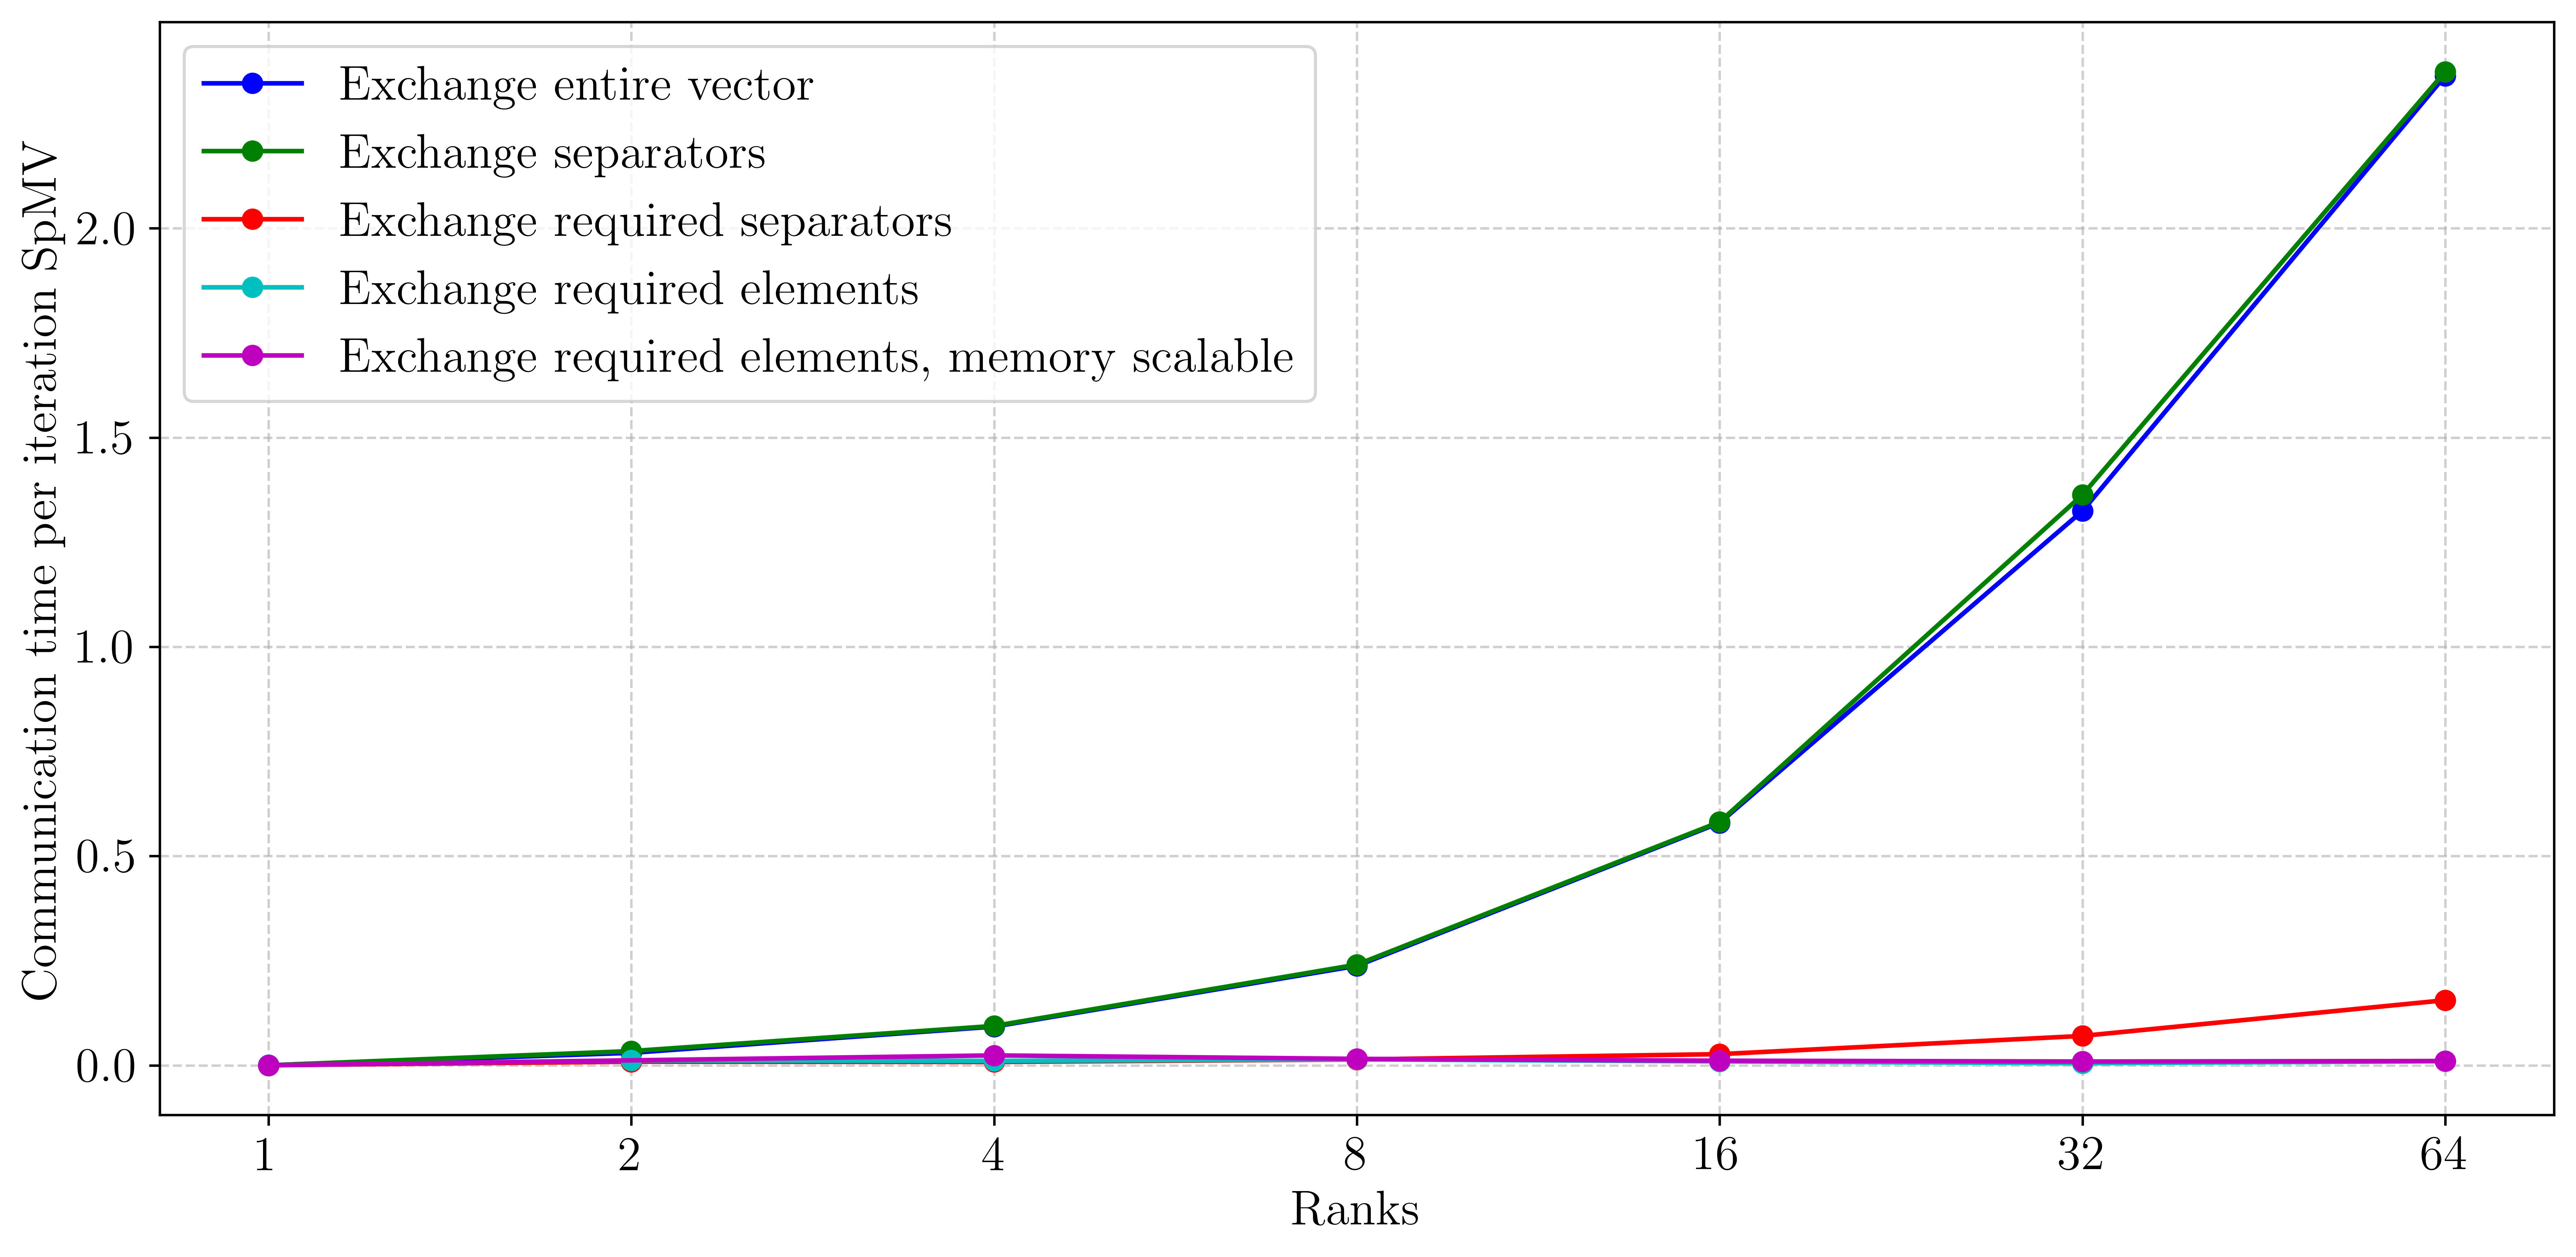
\includegraphics[width=0.95\textwidth]{nlpkkt200_tcomm_single_defq.png}
    \end{center}
    \caption{}
    \label{fig:nlpkkt200_tcomm_single_defq.png}
\end{figure}

\begin{figure}[H]
    \begin{center}
        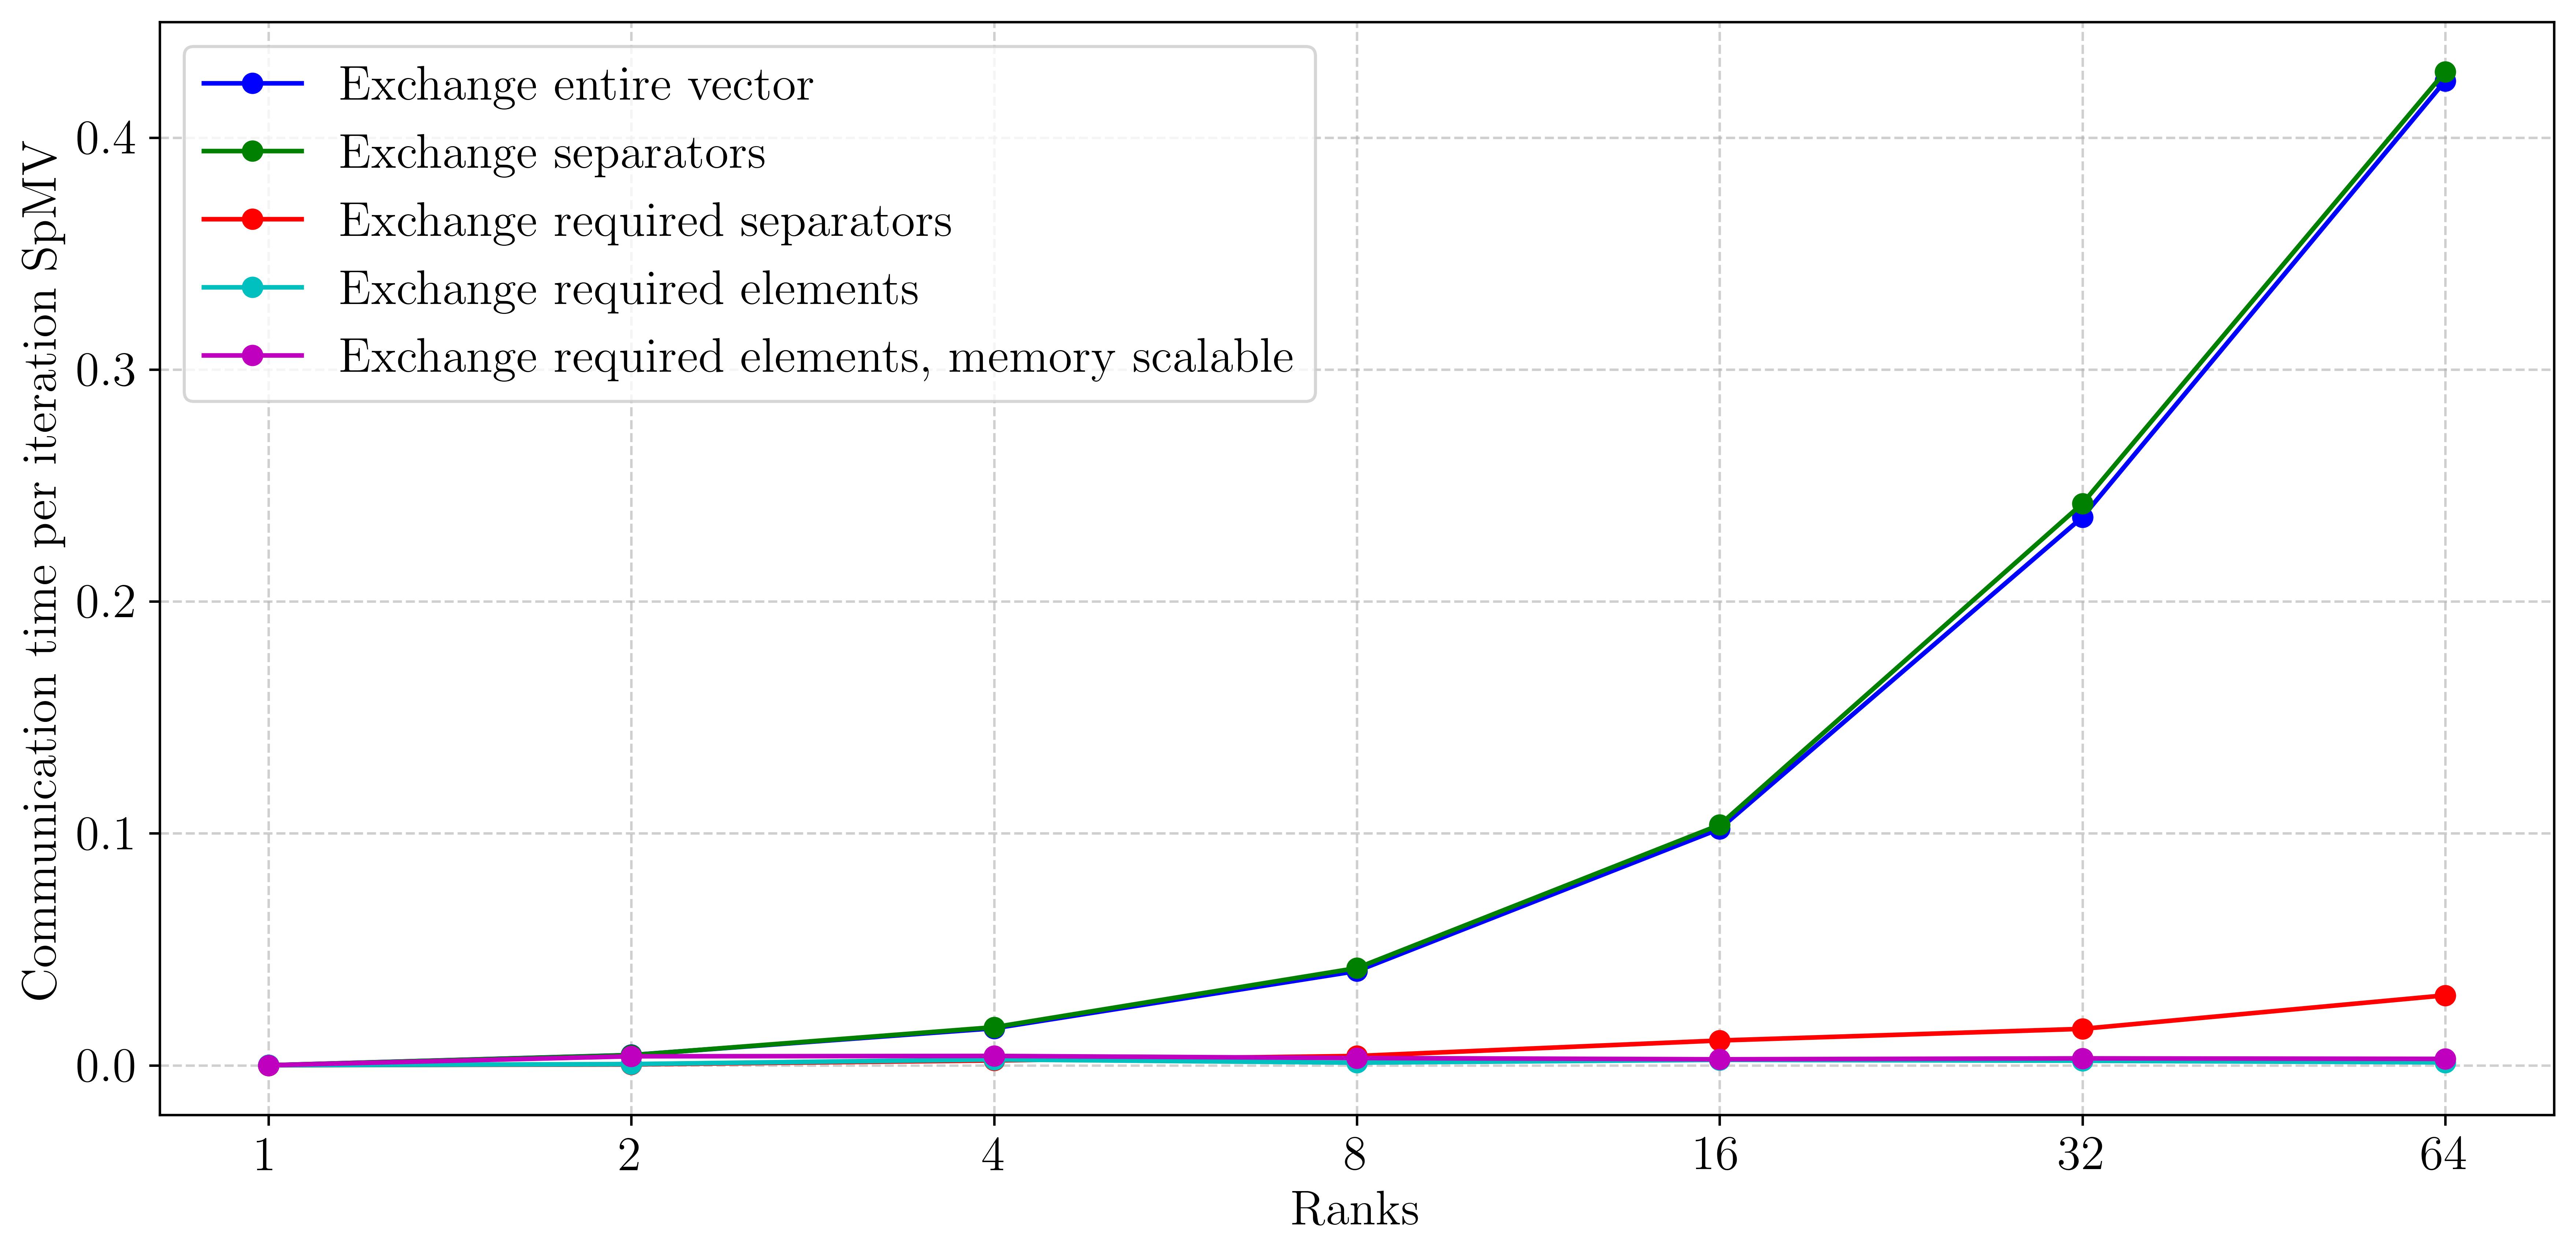
\includegraphics[width=0.95\textwidth]{Bump_2911_tcomm_single_defq.png}
    \end{center}
    \caption{}
    \label{fig:Bump_2911_tcomm_single_defq.png}
\end{figure}

\begin{figure}[H]
    \begin{center}
        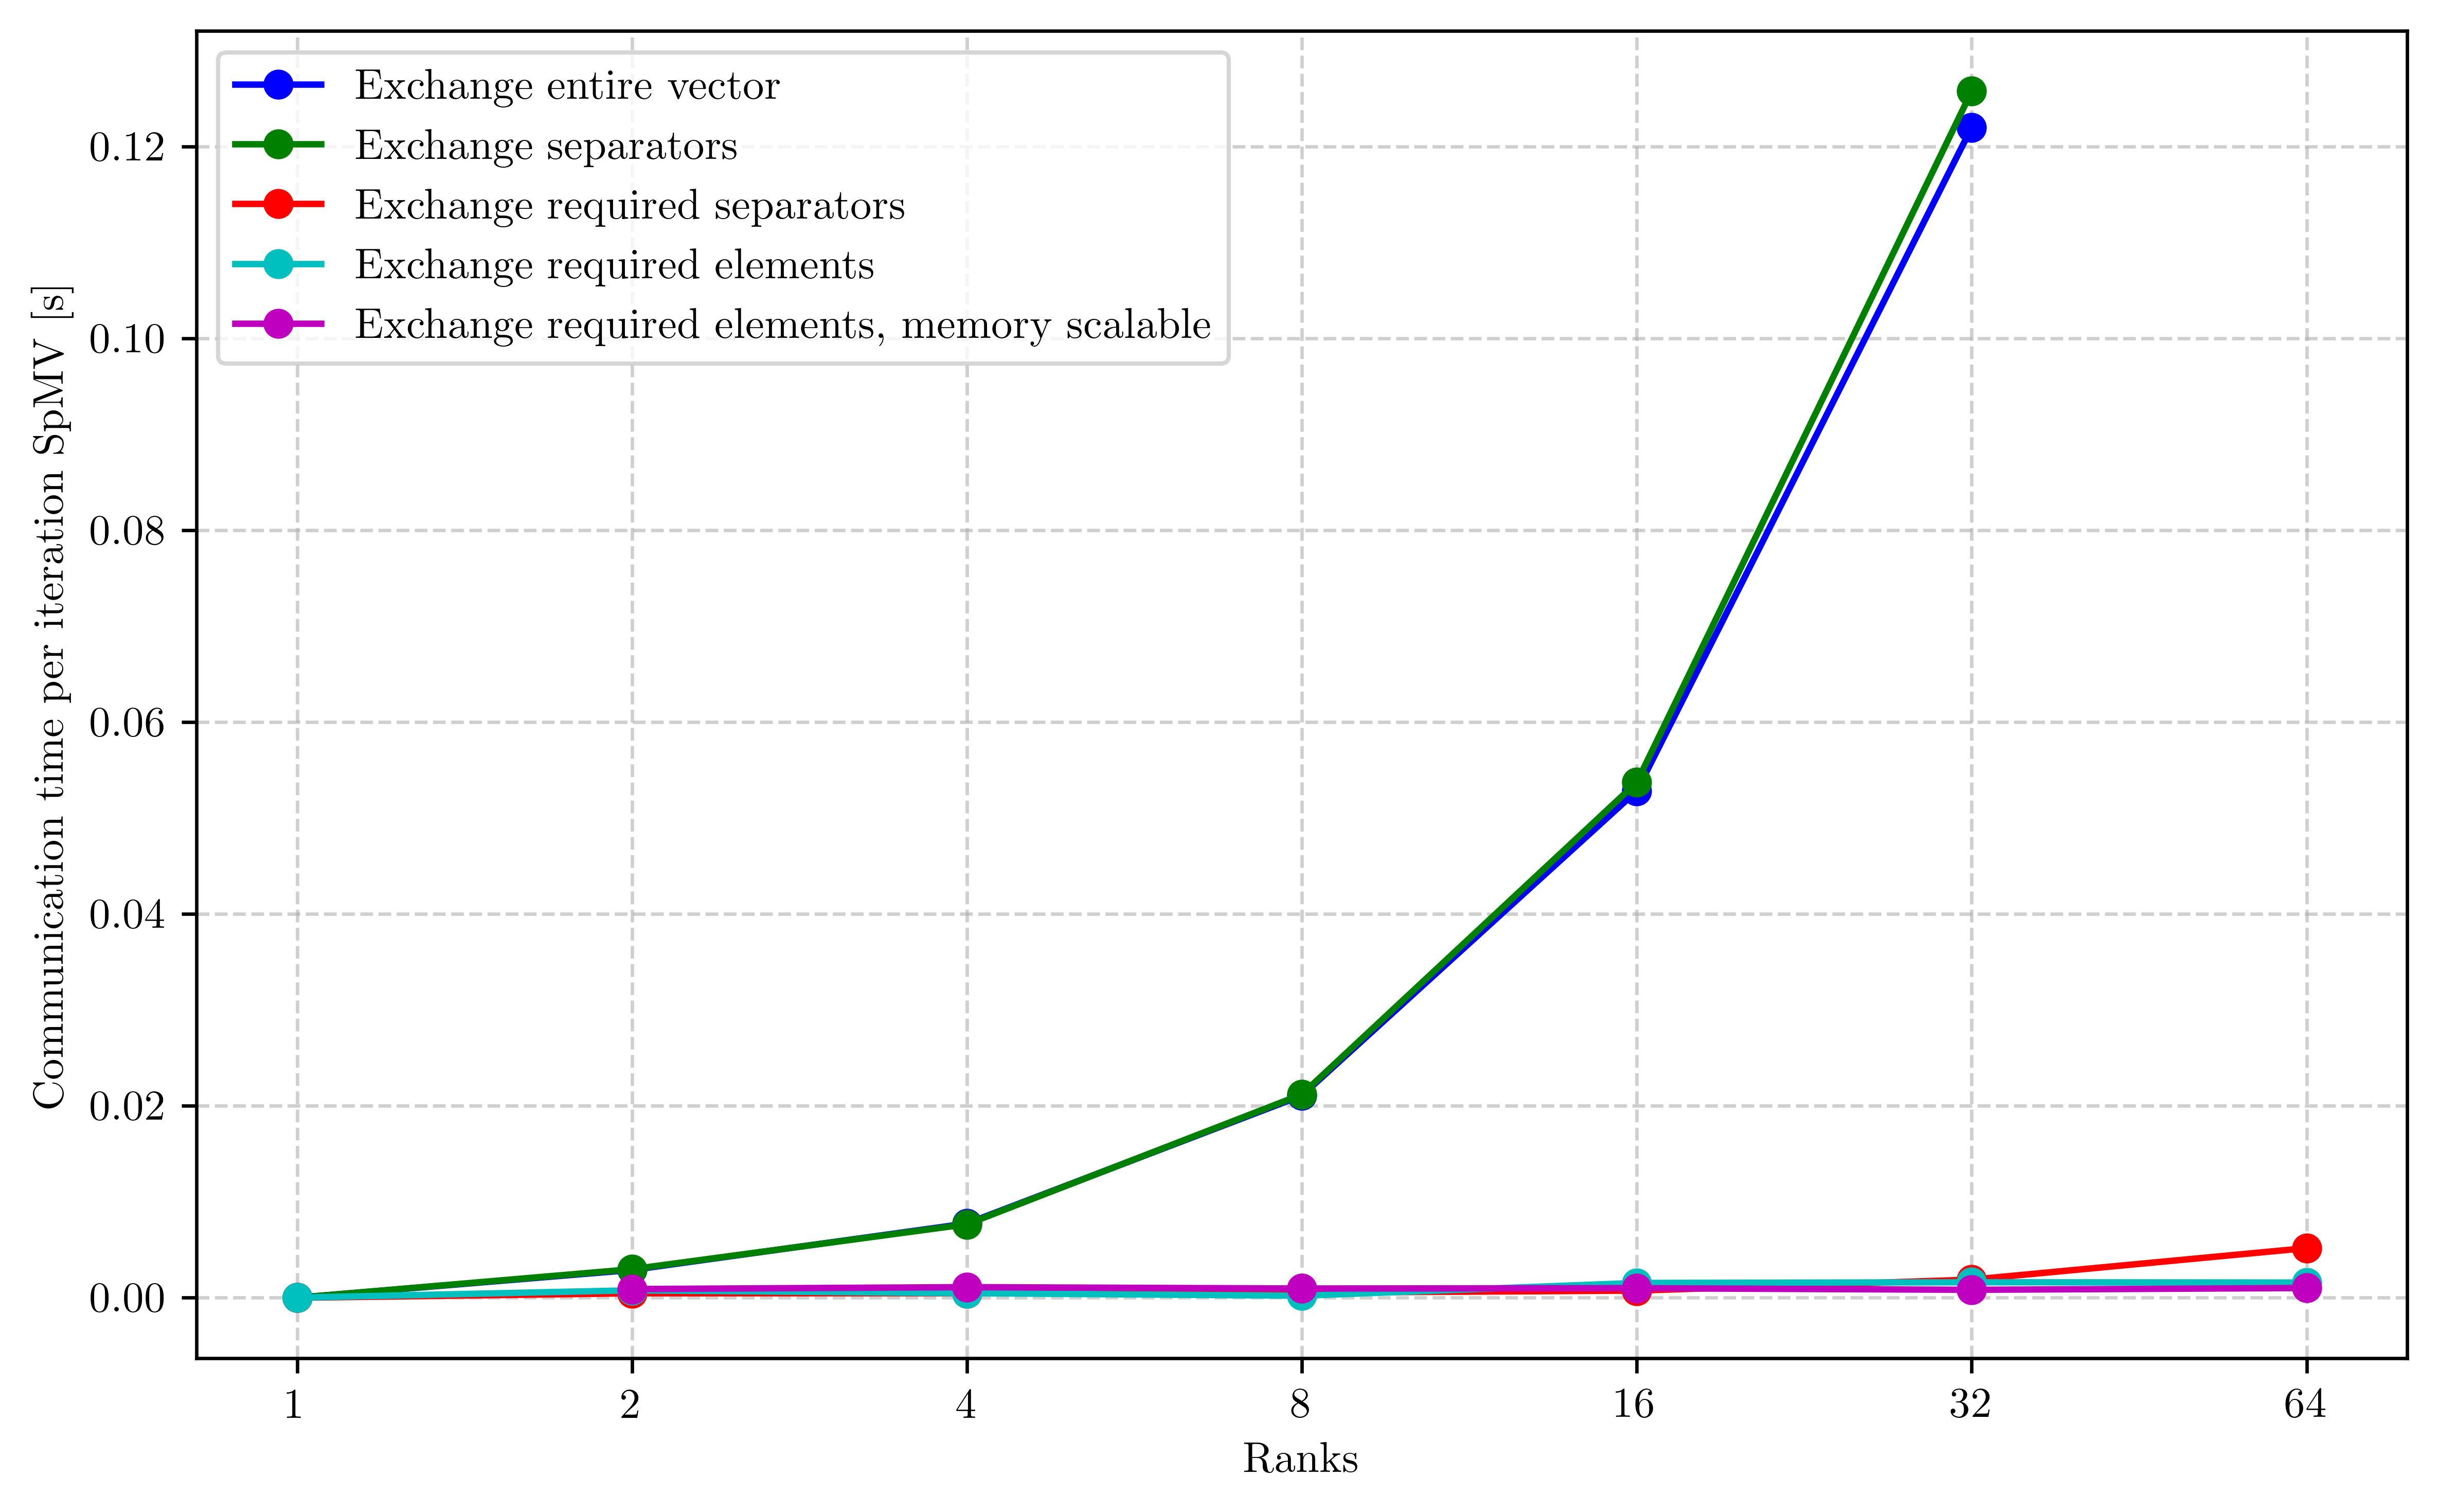
\includegraphics[width=0.95\textwidth]{af_shell10_tcomm_single_defq.png}
    \end{center}
    \caption{}
    \label{fig:af_shell10_tcomm_single_defq.png}
\end{figure}

\begin{figure}[H]
    \begin{center}
        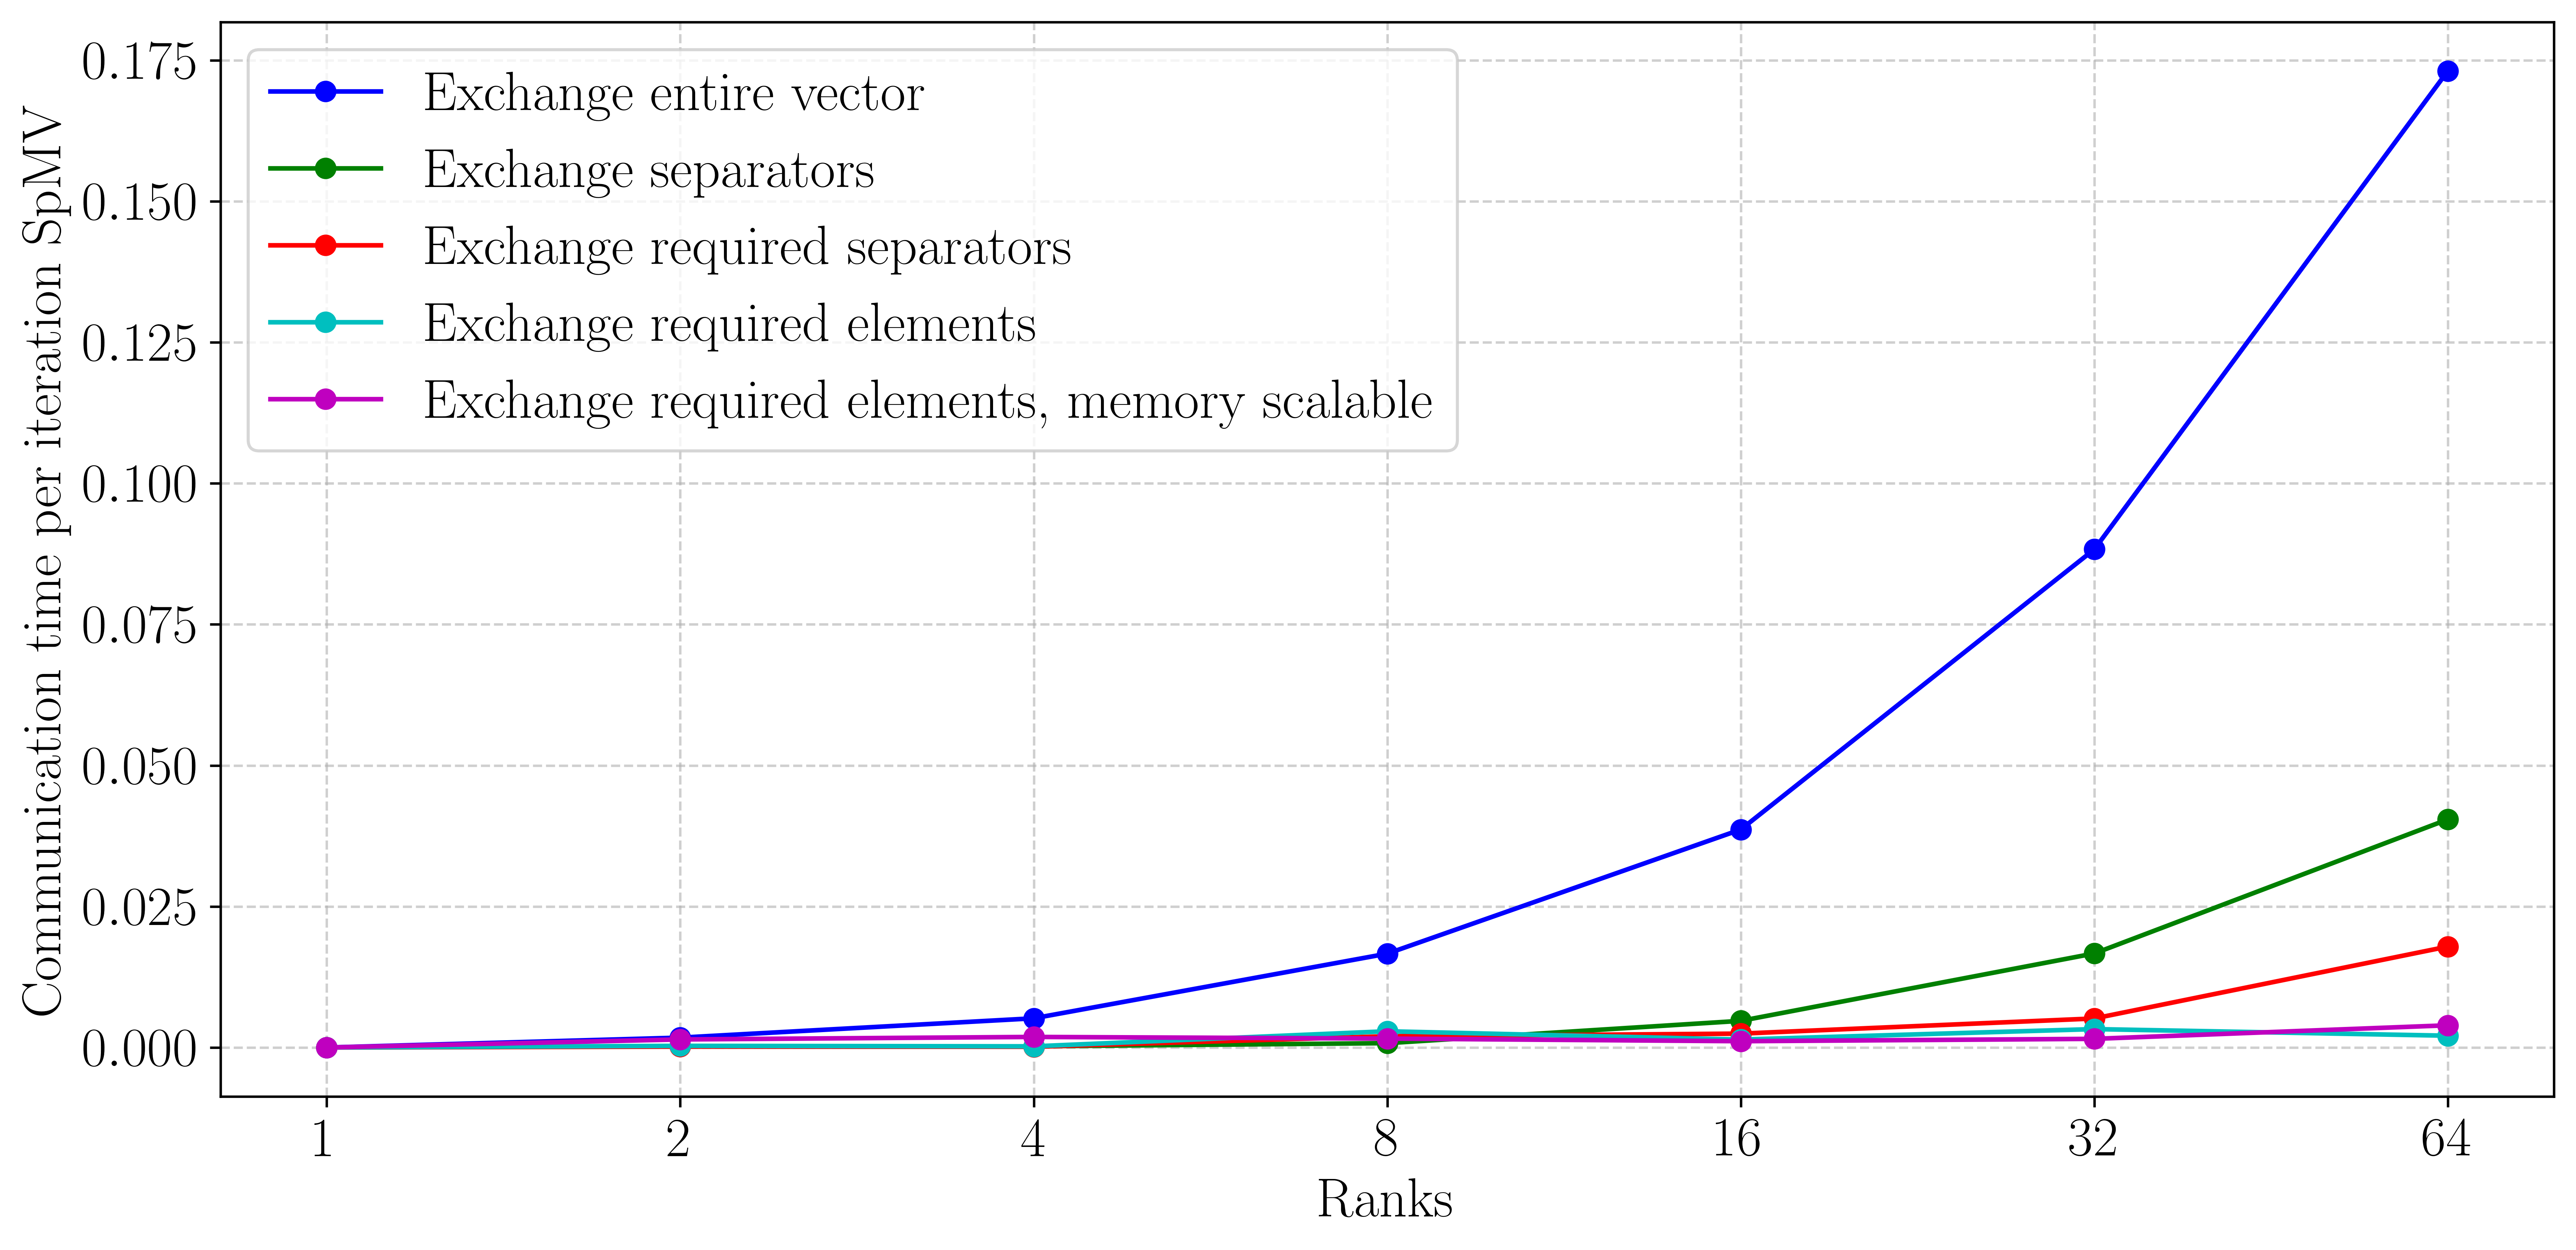
\includegraphics[width=0.95\textwidth]{dielFilterV3real_tcomm_single_defq.png}
    \end{center}
    \caption{}
    \label{fig:dielFilterV3real_tcomm_single_defq.png}
\end{figure}

\begin{figure}[H]
    \begin{center}
        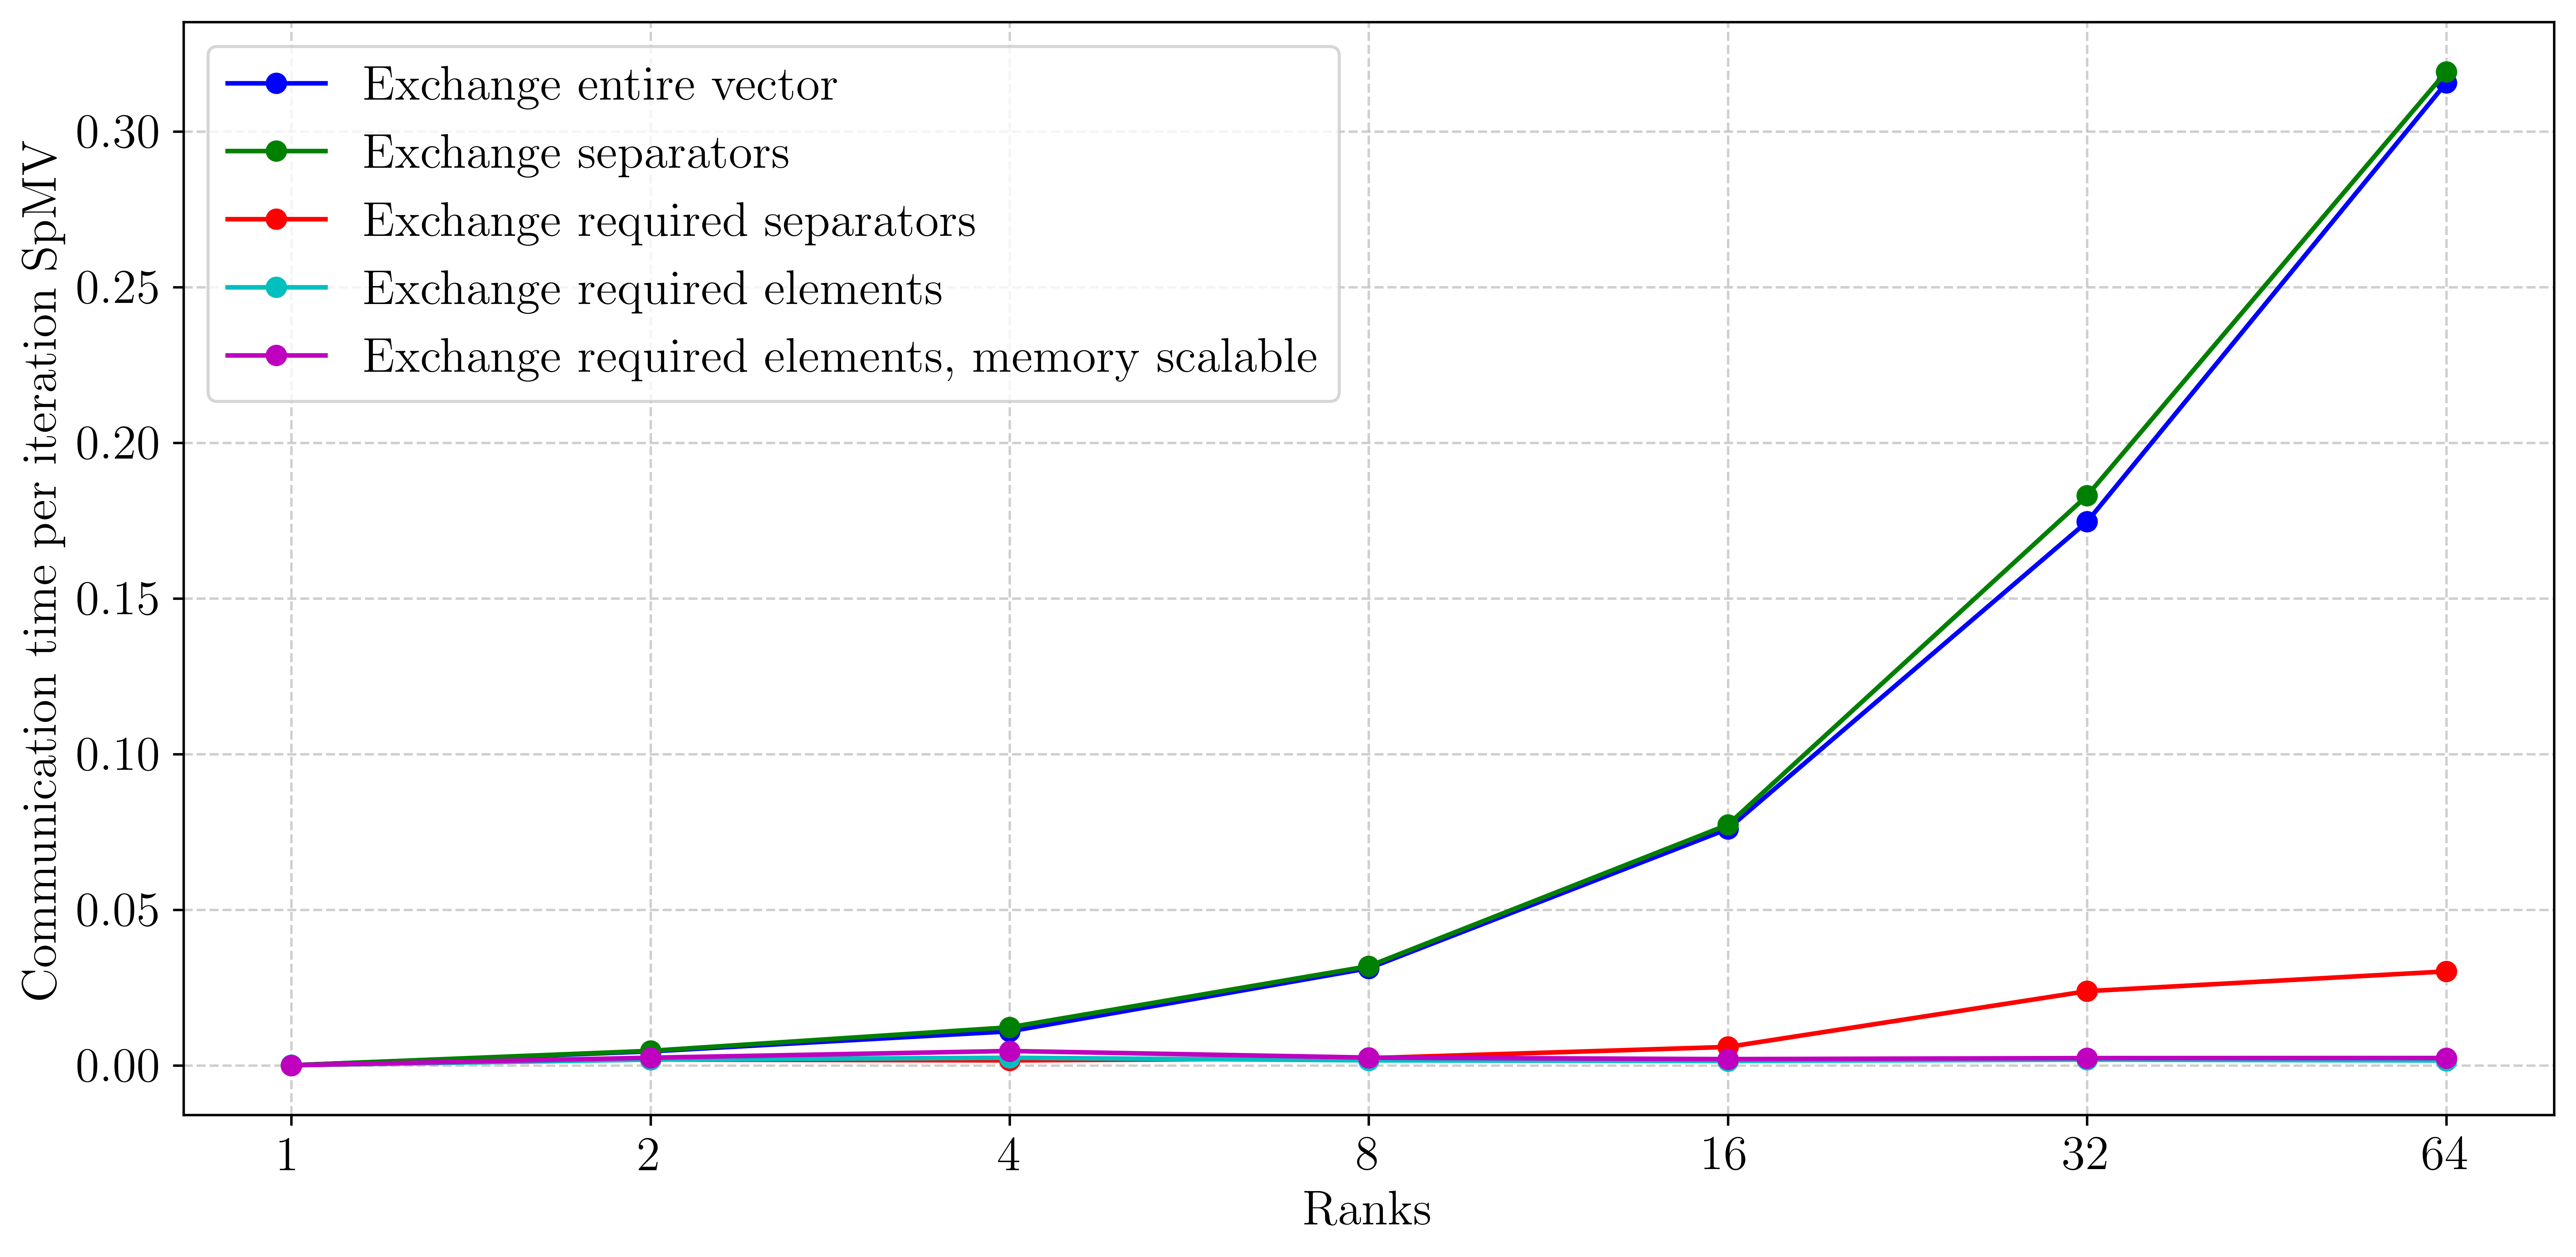
\includegraphics[width=0.95\textwidth]{Cube_Coup_dt0_tcomm_single_defq.png}
    \end{center}
    \caption{}
    \label{fig:Cube_Coup_dt0_tcomm_single_defq.png}
\end{figure}

\begin{figure}[H]
    \begin{center}
        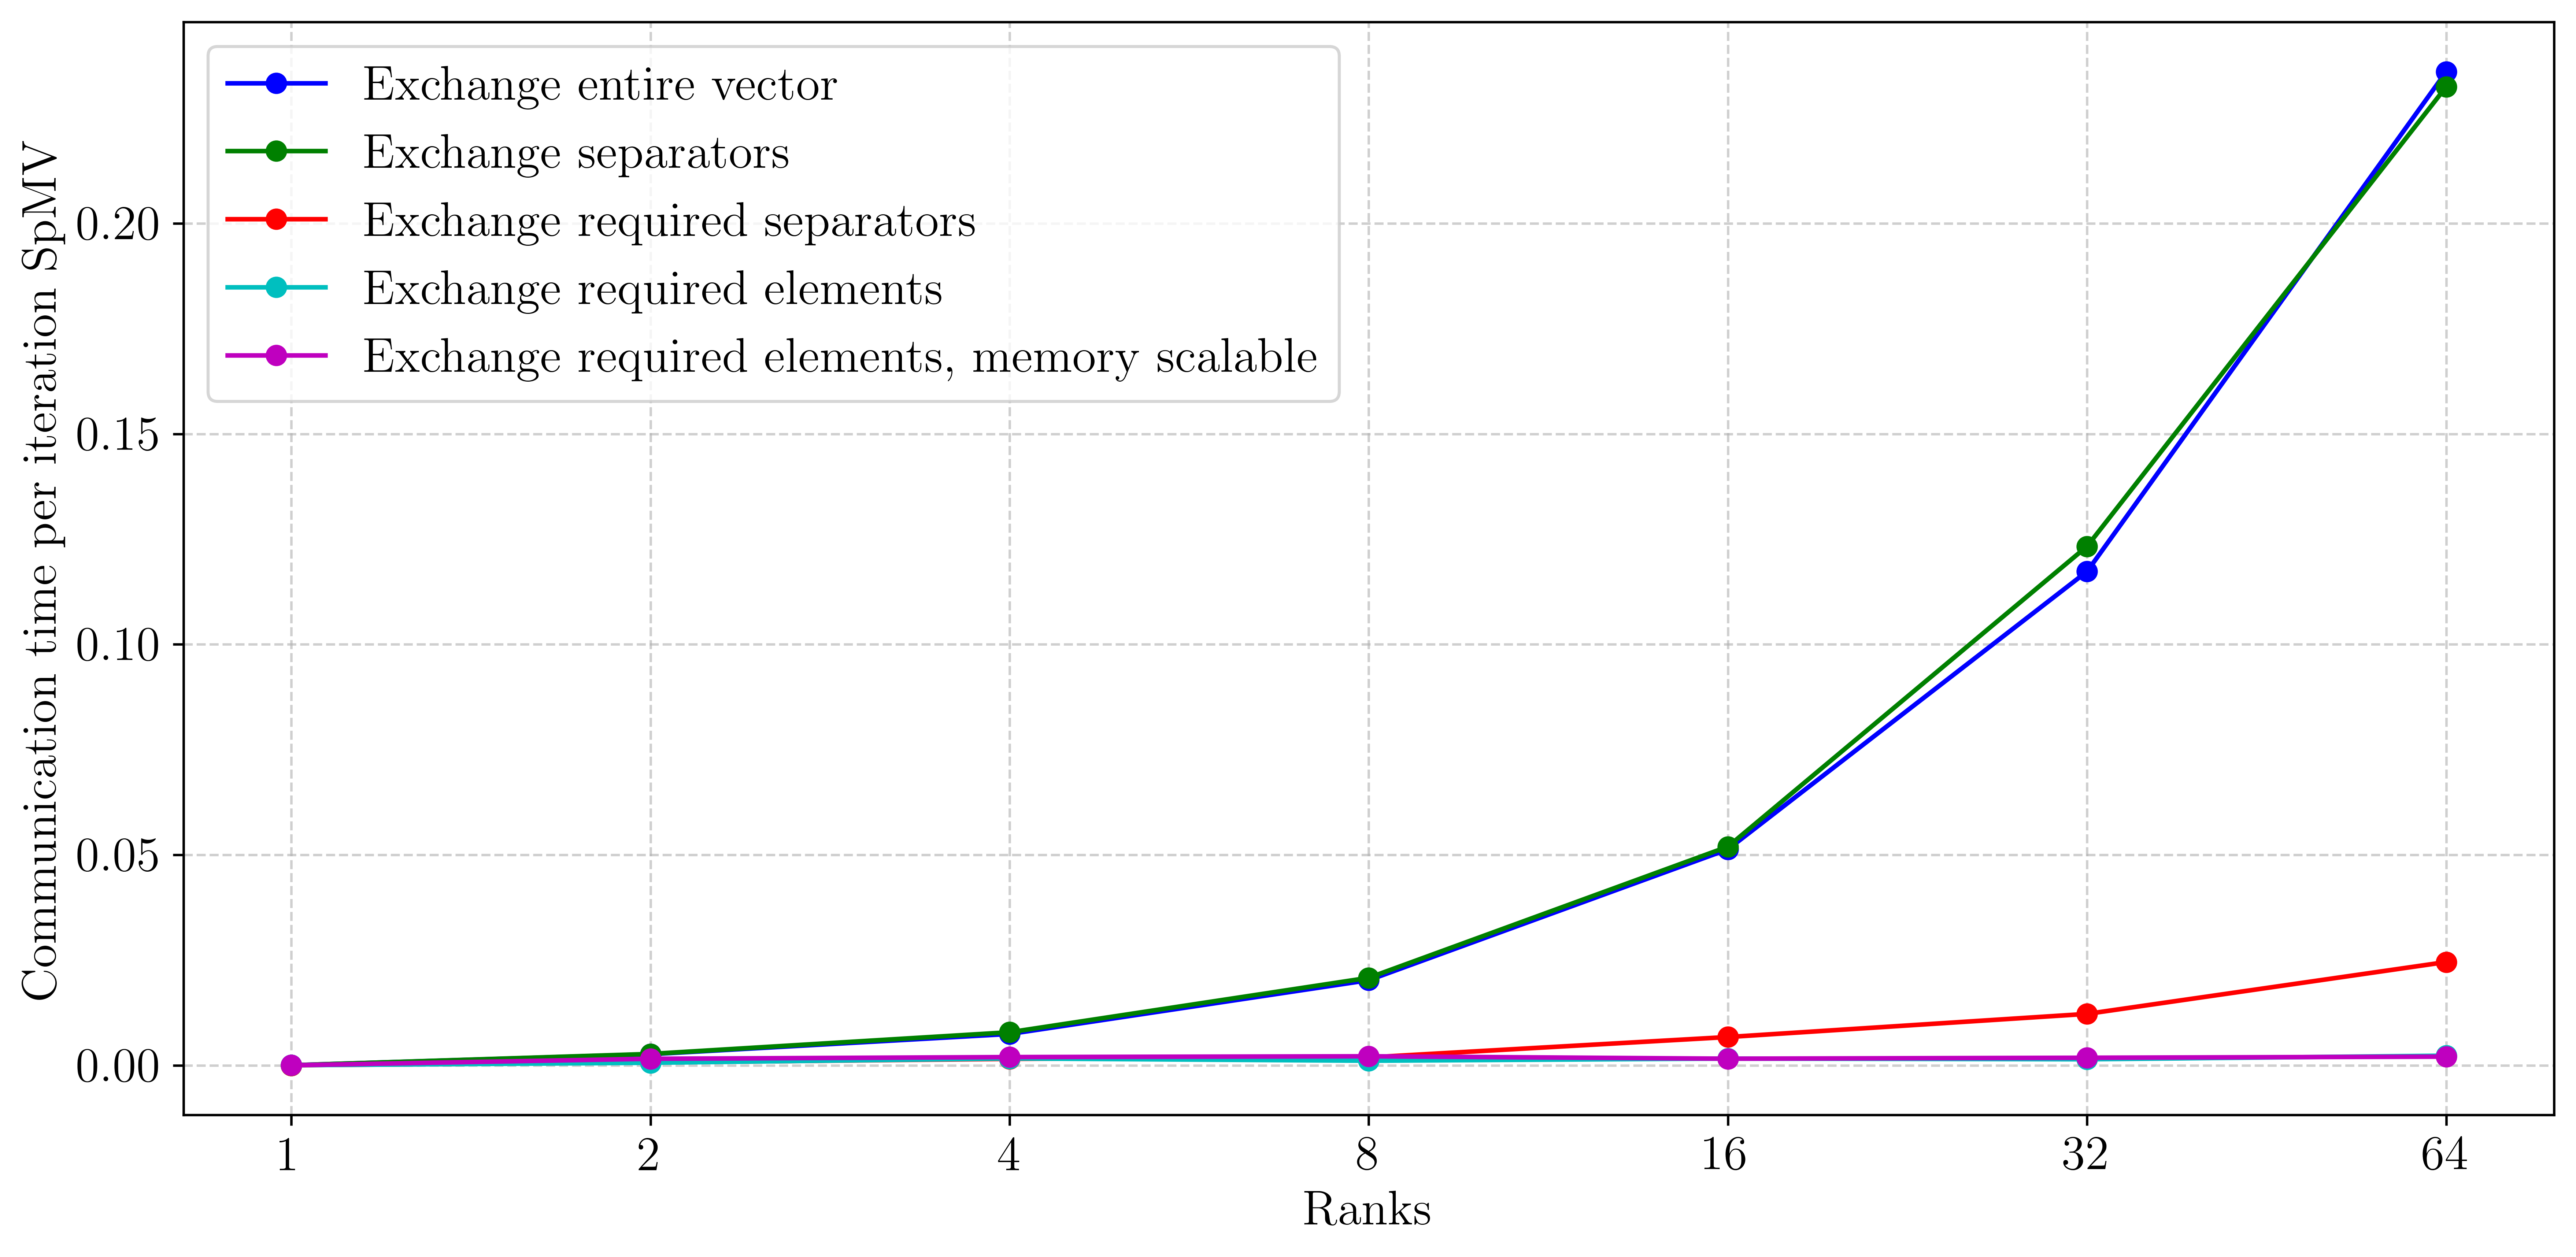
\includegraphics[width=0.95\textwidth]{Long_Coup_dt0_tcomm_single_defq.png}
    \end{center}
    \caption{}
    \label{fig:Long_Coup_dt0_tcomm_single_defq.png}
\end{figure}


% eX3 - High-Performance Computing Reports
%
% Copyright (C) 2020 Simula Research Laboratory
% Authors: James D. Trotter <james@simula.no>
%
% Hardware

\begin{table}[ht]
  \centering
  \linespread{0.85}\renewcommand{\arraystretch}{1.2}
  \setlength{\tabcolsep}{2pt}    % a little padding between columns
  \footnotesize\sffamily
  %--------------------------------------------------------------------------------
  % use tabular* + \extracolsep{\fill} to force it to exactly \textwidth
  \begin{tabular*}{\textwidth}{@{\extracolsep{\fill}}
      l
      >{\raggedleft\arraybackslash}p{0.18\textwidth}
      >{\raggedleft\arraybackslash}p{0.18\textwidth}
      >{\raggedleft\arraybackslash}p{0.18\textwidth}
    @{}}
    \toprule
      & {\small FPGAQ}
      & {\small Rome}
      & {\small Defq} \\
    \midrule
    CPUs
      & \fpgaq{} 
      & \romeq{} 
      & \defq{} \\

    Instr.\ setu w
      & x86-64
      & x86-64
      & x86-64 \\

    Microarch.
      & Zen 3
      & Zen 2
      & Zen 1 \\

    Sockets
      & 2
      & 1
      & 2 \\

    Cores
      & $2\times24$
      & $1\times16$
      & $2\times32$ \\

    Freq.~[GHz]
      & $2.6$--$3.6$
      & $1.5$--$3.3$
      & $2.2$--$3.2$  \\

    \midrule
    L1I/core [KiB]
      & 64
      & 32
      & 64\\

    L1D/core [KiB]
      & 32
      & 32
      & 32 \\

    L2/core [KiB]
      & 512
      & 512
      & 512 \\

    L3/socket [MiB]
      & 128
      & 16
      & 128 \\

    Mem.\ channels
      & $2\times8$
      & $1\times8$
      & $2\times8$ \\

    Bandwidth [GB/s]
      & N/A
      & 204.8
      & N/A\\

    Triad [GB/s]
      & N/A
      & 90.9
      & N/A \\
    \bottomrule
  \end{tabular*}
  \caption{Hardware used in the experiments. STREAM Triad was run with the \texttt{-march=native} and \texttt{-O3} compilation flags.}
  \label{tab:hardware}
\end{table}



% \begin{table*}[thb]
%   \centering
%   \caption{\small Hardware used in our experiments. STREAM Triad \cite{mccalpin1995memory} was run with the \texttt{-march=native} and  \texttt{O3} compilation flags.}
%   \footnotesize
%   \setlength{\tabcolsep}{4pt}
%   \resizebox{\textwidth}{!}{
%   \begin{tabular}{lrrrrrr}
%     \toprule
%     Chip	&	{\scriptsize AMD Epyc}	&	{\scriptsize AMD Epyc}	&	{\scriptsize AMD Epyc}	&	{\scriptsize AMD Epyc}	&	{\scriptsize Intel Xeon}	&	{\scriptsize Intel Xeon}	\\
%     Model	&	{\scriptsize 7763}	&	{\scriptsize 7601}	&	{\scriptsize  7413}	&	{\scriptsize 7302P}	&	{\scriptsize Gold 6130}	&	{\scriptsize Platinum 8360Y}	\\
%     \midrule													
%     Instruction set	&	x86-64	&	x86-64	&	x86-64	&	x86-64	&	x86-64	&	x86-64	\\
%     Microarchitecture	&	Zen3	&	Zen	&	Zen3	&	Zen2	&	 Skylake (server) 	&	Ice Lake (server)  	\\
%     Cores/Threads	&	2 $\times$ 64/128	&	2 $\times$ 32/64	&	2 $\times$ 24/48	&	16/32	&	 2 $\times$ 32/64     	&	  2 $\times$ 36/72 	\\
%     Core frequency(GHz)	&	2.45 to 5.5	&	2.7 to 3.2	&	2.65 to 3.6	&	3.0 to 3.3	&	 1.9 to 3.6  	&	  1.8 to 3.6 	\\
%     L1I/L1D/L2 (KiB per core)	&	32/32/512	&	64/32/512	&	32/32/512	&	32/32/512	&	32/32/1024	&	 32/48/1280 	\\
%     L3 cache (MiB)	&	2 $\times$ 256 (8 $\times$ 32)	&	2 $\times$ 64 (8 $\times$ 8)	&	2 $\times$ 128 (4 $\times$ 32)	&
%                                                                                                                                                  128 (8 $\times$ 16)		&	2 $\times$ 22 	&	2 $\times$ 54	\\
%     Memory Channels	&	 2 $\times$ 8 	&	 2 $\times$ 8 	&	 2 $\times$ 8 	&	8	&	2 $\times$ 6	&	 2 $\times$ 8 	\\
%     Total Memory (GB)	&	2048	&	2048	&	512	&	256	&	384	&	2048	\\
%     Max.~bandwidth (GB/s)	&	381.4	&	340.8	&	381.4	&	190.7	&	238.4	&	381.4	\\
%     STREAM Triad (GB/s)	&	200.8	&	161.4	&	200.8	&	90.6	&	147.1	&	293.1	\\
%     \addlinespace
%     \bottomrule
    
%   \end{tabular}}
%   \label{tbl:hardware}
% \end{table*}
% %milan 8*32




    %  Chip & {\scriptsize AMD Epyc} & {\scriptsize Intel Xeon } & {\scriptsize AMD Epyc } & {\scriptsize Cavium ThunderX2} & {\scriptsize HiSilicon Kunpeng} \\
    %  Model & {\scriptsize 7302P} & {\scriptsize Gold 6130} & {\scriptsize 7601} & {\scriptsize  CN9980} & {\scriptsize 920-6428} \\ 
    % \midrule
    % Instruction set      & x86-64             & x86-64           & x86-64    & ARMv8.1  & ARMv8.2    \\
    % Microarchitecture    & Zen 2       & Skylake (server) & Zen      & 	Vulcan  & TaiShan v110      \\
    % Cores/Threads        & 16/32              & 2 $\times$ 32/64     & 2 $\times$ 32/64 &  2 $\times$ 32/128   &  2 $\times$ 64/64    \\
    % Core frequency (GHz)      & 3.0 to 3.3       & 1.9 to 3.6  & 2.7 to 3.2 &  2.0 to 2.5  &  2.8   \\
    % L1I/L1D/L2 (KiB per core)     & 32/32/512     & 32/32/1024    & 64/32/512   & 32/32/256 & 64/64/512  \\  
    % L3 cache (MiB per socket)  & 128 (8x16) 	  & 22 (16x1.375)   & 64	(8x8)  & 32	(32x1)  & 64	(64x1)  \\
    % Memory Channels        &  8 & 2 $\times$ 6  & 2 $\times$ 8 & 2 $\times$ 8 & 2 $\times$ 8  \\
    % Total Memory (GB)        & 256 & 384 & 2048 & 1024 & 1024  \\  
    % Max.~bandwidth (GB/s)      & 204.8       & 238.4        & 340.8  & 317.9   & 381.4   \\
    %       STREAM Triad  (GB/s)             & 90.6       & 147.1      & 161.4  &  173.3 &  193.5  \\
                         
    %                      \addlin


